% Options for packages loaded elsewhere
\PassOptionsToPackage{unicode}{hyperref}
\PassOptionsToPackage{hyphens}{url}
\PassOptionsToPackage{dvipsnames,svgnames,x11names}{xcolor}
%
\documentclass[
]{article}

\usepackage{amsmath,amssymb}
\usepackage{iftex}
\ifPDFTeX
  \usepackage[T1]{fontenc}
  \usepackage[utf8]{inputenc}
  \usepackage{textcomp} % provide euro and other symbols
\else % if luatex or xetex
  \usepackage{unicode-math}
  \defaultfontfeatures{Scale=MatchLowercase}
  \defaultfontfeatures[\rmfamily]{Ligatures=TeX,Scale=1}
\fi
\usepackage[]{palatino}
\ifPDFTeX\else  
    % xetex/luatex font selection
\fi
% Use upquote if available, for straight quotes in verbatim environments
\IfFileExists{upquote.sty}{\usepackage{upquote}}{}
\IfFileExists{microtype.sty}{% use microtype if available
  \usepackage[]{microtype}
  \UseMicrotypeSet[protrusion]{basicmath} % disable protrusion for tt fonts
}{}
\makeatletter
\@ifundefined{KOMAClassName}{% if non-KOMA class
  \IfFileExists{parskip.sty}{%
    \usepackage{parskip}
  }{% else
    \setlength{\parindent}{0pt}
    \setlength{\parskip}{6pt plus 2pt minus 1pt}}
}{% if KOMA class
  \KOMAoptions{parskip=half}}
\makeatother
\usepackage{xcolor}
\setlength{\emergencystretch}{3em} % prevent overfull lines
\setcounter{secnumdepth}{5}
% Make \paragraph and \subparagraph free-standing
\makeatletter
\ifx\paragraph\undefined\else
  \let\oldparagraph\paragraph
  \renewcommand{\paragraph}{
    \@ifstar
      \xxxParagraphStar
      \xxxParagraphNoStar
  }
  \newcommand{\xxxParagraphStar}[1]{\oldparagraph*{#1}\mbox{}}
  \newcommand{\xxxParagraphNoStar}[1]{\oldparagraph{#1}\mbox{}}
\fi
\ifx\subparagraph\undefined\else
  \let\oldsubparagraph\subparagraph
  \renewcommand{\subparagraph}{
    \@ifstar
      \xxxSubParagraphStar
      \xxxSubParagraphNoStar
  }
  \newcommand{\xxxSubParagraphStar}[1]{\oldsubparagraph*{#1}\mbox{}}
  \newcommand{\xxxSubParagraphNoStar}[1]{\oldsubparagraph{#1}\mbox{}}
\fi
\makeatother


\providecommand{\tightlist}{%
  \setlength{\itemsep}{0pt}\setlength{\parskip}{0pt}}\usepackage{longtable,booktabs,array}
\usepackage{calc} % for calculating minipage widths
% Correct order of tables after \paragraph or \subparagraph
\usepackage{etoolbox}
\makeatletter
\patchcmd\longtable{\par}{\if@noskipsec\mbox{}\fi\par}{}{}
\makeatother
% Allow footnotes in longtable head/foot
\IfFileExists{footnotehyper.sty}{\usepackage{footnotehyper}}{\usepackage{footnote}}
\makesavenoteenv{longtable}
\usepackage{graphicx}
\makeatletter
\def\maxwidth{\ifdim\Gin@nat@width>\linewidth\linewidth\else\Gin@nat@width\fi}
\def\maxheight{\ifdim\Gin@nat@height>\textheight\textheight\else\Gin@nat@height\fi}
\makeatother
% Scale images if necessary, so that they will not overflow the page
% margins by default, and it is still possible to overwrite the defaults
% using explicit options in \includegraphics[width, height, ...]{}
\setkeys{Gin}{width=\maxwidth,height=\maxheight,keepaspectratio}
% Set default figure placement to htbp
\makeatletter
\def\fps@figure{htbp}
\makeatother
% definitions for citeproc citations
\NewDocumentCommand\citeproctext{}{}
\NewDocumentCommand\citeproc{mm}{%
  \begingroup\def\citeproctext{#2}\cite{#1}\endgroup}
\makeatletter
 % allow citations to break across lines
 \let\@cite@ofmt\@firstofone
 % avoid brackets around text for \cite:
 \def\@biblabel#1{}
 \def\@cite#1#2{{#1\if@tempswa , #2\fi}}
\makeatother
\newlength{\cslhangindent}
\setlength{\cslhangindent}{1.5em}
\newlength{\csllabelwidth}
\setlength{\csllabelwidth}{3em}
\newenvironment{CSLReferences}[2] % #1 hanging-indent, #2 entry-spacing
 {\begin{list}{}{%
  \setlength{\itemindent}{0pt}
  \setlength{\leftmargin}{0pt}
  \setlength{\parsep}{0pt}
  % turn on hanging indent if param 1 is 1
  \ifodd #1
   \setlength{\leftmargin}{\cslhangindent}
   \setlength{\itemindent}{-1\cslhangindent}
  \fi
  % set entry spacing
  \setlength{\itemsep}{#2\baselineskip}}}
 {\end{list}}
\usepackage{calc}
\newcommand{\CSLBlock}[1]{\hfill\break\parbox[t]{\linewidth}{\strut\ignorespaces#1\strut}}
\newcommand{\CSLLeftMargin}[1]{\parbox[t]{\csllabelwidth}{\strut#1\strut}}
\newcommand{\CSLRightInline}[1]{\parbox[t]{\linewidth - \csllabelwidth}{\strut#1\strut}}
\newcommand{\CSLIndent}[1]{\hspace{\cslhangindent}#1}

\usepackage[noblocks]{authblk}
\renewcommand*{\Authsep}{, }
\renewcommand*{\Authand}{, }
\renewcommand*{\Authands}{, }
\renewcommand\Affilfont{\small}
\usepackage{amssymb}
\usepackage{booktabs} % Add to your preamble for cleaner table lines
\usepackage{makecell} % Add to your preamble for multi-line cells
\usepackage{tikz}
\usetikzlibrary{arrows.meta, shapes.geometric}

%% Define TikZ arrow styles
\newcommand{\starstar}{% 
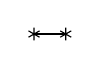
\begin{tikzpicture}[baseline=-3pt]
    \draw [{Rays[n=6]}-{Rays[n=6]}] (0,0) -- (0.55,0);
\end{tikzpicture}
}

\newcommand{\circstar}{% 
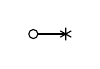
\begin{tikzpicture}
    \draw [{Circle[open]}-{Rays[n=6]}] (0,0) -- (0.55, 0);
\end{tikzpicture}
}

\newcommand{\starcirc}{% 
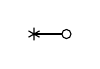
\begin{tikzpicture}
    \draw [{Rays[n=6]}-{Circle[open]}] (0,0) -- (0.55, 0);
\end{tikzpicture}
}

\newcommand{\stararrow}{% 
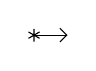
\begin{tikzpicture}
    \draw [{Rays[n=6]}-{Straight Barb[length=2.5pt]}] (0,0) -- (0.5, 0);
\end{tikzpicture}
}

\newcommand{\arrowstar}{% 
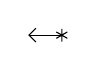
\begin{tikzpicture}
    \draw [{Straight Barb[length=2.5pt]}-{Rays[n=6]}] (0,0) -- (0.5, 0);
\end{tikzpicture}
}

\newcommand{\circarrow}{% 
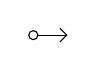
\begin{tikzpicture}
    \draw [{Circle[open]}-{Straight Barb[length=2.5pt]}] (0,0) -- (0.5, 0);
\end{tikzpicture}
}

\newcommand{\tailcirc}{% 
\begin{tikzpicture}[baseline=-3pt] 
    \draw [-{Circle[open]}] (0,0) -- (0.4, 0);
\end{tikzpicture}
}

\newcommand{\circtail}{% 
\begin{tikzpicture}[baseline=-3pt] 
    \draw [{Circle[open]}-] (0,0) -- (0.4, 0);
\end{tikzpicture}
}

\newcommand{\circirc}{% 
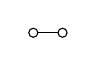
\begin{tikzpicture}[baseline=-3pt] 
    \draw [{Circle[open]}-{Circle[open]}] (0,0) -- (0.5, 0);
\end{tikzpicture}
}

\newcommand{\tailstar}{% 
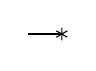
\begin{tikzpicture}[baseline=-3pt] 
    \draw [-{Rays[n=6]}] (0,0) -- (0.5, 0);
\end{tikzpicture}
}

\newcommand{\startail}{% 
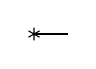
\begin{tikzpicture}
    \draw [{Rays[n=6]}-] (0,0) -- (0.5, 0);
\end{tikzpicture}
}

\newcommand{\tailarrow}{% 
\begin{tikzpicture}
    \draw [-{Straight Barb[length=2.5pt]}](0,0) -- (0.4, 0);
\end{tikzpicture}
}

\newcommand{\arrowtail}{% 
\begin{tikzpicture}
    \draw [{Straight Barb[length=2.5pt]}-](0,0) -- (0.4, 0);
\end{tikzpicture}
}

\newcommand{\arrowarrow}{% 
\begin{tikzpicture}
    \draw [{Straight Barb[length=2.5pt]}-{Straight Barb[length=2.5pt]}](0,0) -- (0.4, 0);
\end{tikzpicture}
}

\newcommand\stackedarrows{%
        \mathrel{\vcenter{\mathsurround0pt
                \ialign{##\crcr
                \noalign{\nointerlineskip}$\arrowtail$\crcr
                \noalign{\nointerlineskip}$\tailarrow$\crcr
                }
        }}%
}
\makeatletter
\@ifpackageloaded{caption}{}{\usepackage{caption}}
\AtBeginDocument{%
\ifdefined\contentsname
  \renewcommand*\contentsname{Table of contents}
\else
  \newcommand\contentsname{Table of contents}
\fi
\ifdefined\listfigurename
  \renewcommand*\listfigurename{List of Figures}
\else
  \newcommand\listfigurename{List of Figures}
\fi
\ifdefined\listtablename
  \renewcommand*\listtablename{List of Tables}
\else
  \newcommand\listtablename{List of Tables}
\fi
\ifdefined\figurename
  \renewcommand*\figurename{Figure}
\else
  \newcommand\figurename{Figure}
\fi
\ifdefined\tablename
  \renewcommand*\tablename{Table}
\else
  \newcommand\tablename{Table}
\fi
}
\@ifpackageloaded{float}{}{\usepackage{float}}
\floatstyle{ruled}
\@ifundefined{c@chapter}{\newfloat{codelisting}{h}{lop}}{\newfloat{codelisting}{h}{lop}[chapter]}
\floatname{codelisting}{Listing}
\newcommand*\listoflistings{\listof{codelisting}{List of Listings}}
\makeatother
\makeatletter
\makeatother
\makeatletter
\@ifpackageloaded{caption}{}{\usepackage{caption}}
\@ifpackageloaded{subcaption}{}{\usepackage{subcaption}}
\makeatother

\ifLuaTeX
  \usepackage{selnolig}  % disable illegal ligatures
\fi
\usepackage{bookmark}

\IfFileExists{xurl.sty}{\usepackage{xurl}}{} % add URL line breaks if available
\urlstyle{same} % disable monospaced font for URLs
\hypersetup{
  pdftitle={Causal Discovery on Precarity and Depression},
  pdfauthor={Kyuri Park; Leonie K. Elsenburg; Mary Nicolao; Karien Stronks; Vítor V. Vasconcelos},
  colorlinks=true,
  linkcolor={blue},
  filecolor={Maroon},
  citecolor={Blue},
  urlcolor={Blue},
  pdfcreator={LaTeX via pandoc}}


\title{Causal Discovery on Precarity and Depression}


\author[1]{Kyuri Park}
\author[2]{Leonie K. Elsenburg}
\author[2]{Mary Nicolao}
\author[2]{Karien Stronks}
\author[1, 3]{Vítor V. Vasconcelos}

\affil[1]{\textit{Computational Science Lab, Informatics Institute, University of Amsterdam, PO Box 94323, Amsterdam, 1090GH, the Netherlands}}
\affil[2]{\textit{Department of Public and Occupational Health, Amsterdam Public Health Research Institute, Amsterdam UMC, University of Amsterdam, Amsterdam, the Netherland}}
\affil[3]{\textit{Institute for Advanced Study, University of Amsterdam, Oude Turfmarkt 147, Amsterdam, 1012GC, the Netherland}}


\date{2025-02-08}
\begin{document}
\maketitle
\begin{abstract}
\noindent Understanding the causal mechanisms linking precariousness and
depression is critical for developing effective interventions. This
study utilizes data from the HELIUS cohort study to explore these
relationships using advanced causal discovery methods. By applying
algorithms such as FCI, and CCI, and combining traditional Gaussian CI
tests with non-parametric approaches like RCoT, we investigate how
different indicators of precariousness---including factors related to
employment, social relations and relational stress, financial situation,
and housing---affect depressed mood, both as a sum score and at the
individual symptom level. Our findings reveal that relational stress
consistently emerges as a potential causal factor for depressed mood,
while symptoms such as sleep disturbances, guilt, and anhedonia are
particularly sensitive to external stressors, acting as potential early
warning signals or intervention points for prevention. Moreover, the
results highlight complexities in the data, including the influence of
latent confounders and the challenges of capturing cyclic relationships.
Despite some limitations, such as unresolved ambiguities in causal
directions and challenges with mixed data distributions, this study
demonstrates the utility of causal discovery tools in disentangling the
intricate interplay between social and mental health dynamics. By
mapping these causal structures into computational models, future
research can simulate intervention effects, providing actionable
insights to mitigate the impact of precariousness on mental health. This
study serves as a foundational effort, offering both methodological
advancements and practical implications for addressing depression at a
population level.
\end{abstract}

\renewcommand*\contentsname{Table of contents}
{
\hypersetup{linkcolor=}
\setcounter{tocdepth}{3}
\tableofcontents
}

\section{Introduction}\label{introduction}

Mental health problems in urban areas have been reported to be on the
rise the complexity of mental health systems presents significant
challenges in understanding the underlying mechanisms driving these
issues, let alone planning effective interventions.

Research has aimed to identify underlying factors contributing to mental
health problems. Recent research looked into the association between
mental health and indicators of precariousness in various dimensions of
life, indicating a high level of uncertainty and instability in people's
lives, such as factors related to employment, social relations,
finances, housing, and culture (ref Leonie's paper). This comprehensive
perspective on precariousness helped to highlight how different aspects
of life may be interconnected. While this research has advanced our
understanding of which indicators of precariousness are related to
mental health, a key question remains unanswered: how do these factors
influence mental health? Specifically, the lack of directional
information --- knowing what influences what --- limits our ability to
identify and prioritize effective intervention targets.

This study aims to investigate the causal relationships between
different dimensions of precariousness and mental health outcomes, to
with a specific focus on depression, the most prevalent mental health
issue. Using causal discovery methods, we explore how different aspects
of precariousness influence depression and delve deeper into the
dynamics at the symptom level. By examining individual depressive
symptoms, we aim to identify which symptoms may act as initiators by
being particularly sensitive to precariousness. Through this analysis,
our goal is to uncover the causal mechanisms underlying mental health
challenges and provide a foundation for developing more effective and
targeted interventions.

\section{Methods}\label{methods}

\subsection{Data}\label{data}

We use data from the HELIUS study, a multi-ethnic cohort that includes
participants of Dutch, Turkish, Moroccan, Surinamese and Ghanaian origin
(Snijder et al., 2017). To operationalize precariousness factors, we
draw on the framework outlined in previous research (i.e., Leonie's
paper) and select a set of relevant variables.

To ensure a robust representation of each precariousness factor, we
conducted various exploratory analyses to identify consistent and
meaningful factor structures. Based on these analyses, we identified
five precariousness factors, including two related to recent stressors,
each comprising multiple variables as outlined below. Detailed
information on the exploratory analyses can be found in the
\hyperref[sec-appendix]{Appendix}.

\begin{itemize}
\tightlist
\item
  Employment precariousness: \texttt{emp\_stat}, \texttt{work\_sit}.
\item
  Social precariousness: \texttt{soc\_freq}, \texttt{soc\_adq}.
\item
  Housing precariousness: \texttt{nb\_safe}, \texttt{nb\_res},
  \texttt{nb\_rent}, \texttt{cul\_rec}.
\item
  Recent relational stressors: \texttt{frd\_brk12}, \texttt{conf12}.
\item
  Recent financial stressors: \texttt{fincri12}, \texttt{inc\_diff}.
\end{itemize}

After preprocessing, the HELIUS dataset comprises 21,628 samples. Along
with the five precariousness factors, we also compute an overall
precarity score as the combined value of these factors. Additionally,
PHQ-9 scores are included to represent depression, both as a total sum
score and as individual symptom scores. In the subsequent causal
discovery analysis, we examine the relationship between depression and
precarity using both aggregated sum scores and their individual-level
representations. Refer to Figure~\ref{fig-dist} for the overall
distributions of the variables used in the analysis.

\begin{figure}

\centering{

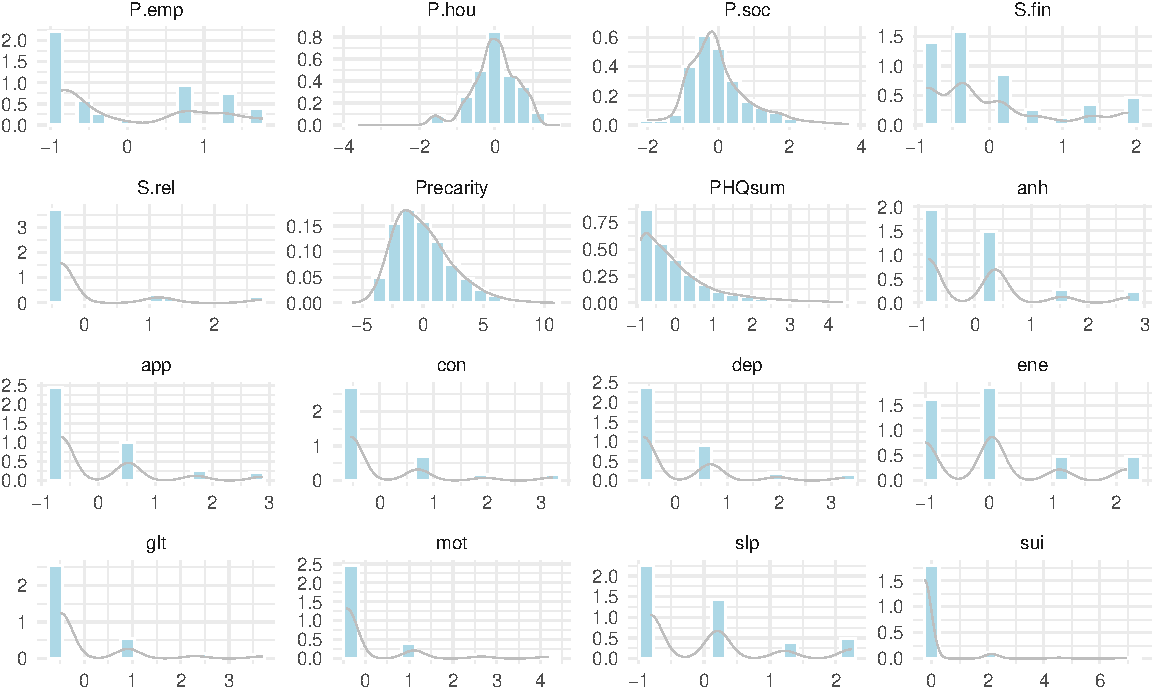
\includegraphics[width=0.9\textwidth,height=\textheight]{draft_v1_files/figure-pdf/fig-dist-1.pdf}

}

\caption{\label{fig-dist}Distributions of variables with density
overlay. \emph{P.emp} = employment precariousness; \emph{P.hou} =
housing precariousness; \emph{P.soc} = social precariousness;
\emph{S.fin} = recent financial stressors; \emph{S.rel} = recent
relational stressors; \emph{Precarity} = overall precarity;
\emph{PHQsum} = PHQ-9 sum score; \emph{anh} = anhedonia; \emph{app} =
appetite; \emph{con} = concentration; \emph{dep} = depressed mood;
\emph{ene} = energy; \emph{glt} = guilty; \emph{mot} = motor; \emph{sui}
= suicidal}

\end{figure}%

\subsection{Causal Discovery}\label{causal-discovery}

There are numerous causal discovery algorithms available; however, in
this study, we focus on algorithms suited to the potential cyclic
relationships within our system. Specifically, we use FCI (Fast Causal
Inference) and CCI (Cyclic Causal Inference), both capable of accounting
for such cycles under certain conditions (Mooij \& Claassen, 2020;
Strobl, 2019). Additionally, we include the PC algorithm as a reference,
given its simplicity and prominence as one of the most widely known
causal discovery methods (Spirtes et al., 2001).

\begin{table}[ht]
\centering
\small % Make the font size smaller
\caption{Assumptions of causal discovery algorithms}
\begin{tabular}{lccccc}
\toprule
Algorithm & Acyclicity & \makecell{Causal \\ sufficiency} & 
\makecell{Absence of \\ selection bias} & Linearity & Output \\ 
\midrule
PC  & $\checkmark$ & $\checkmark$ & $\checkmark$ & $\checkmark$ & CPDAG \\ 
FCI & $-^{a}$ & $\checkmark$ & $-^{a}$ & $-^{a}$ & PAG \\ 
CCI & x & x & x & $\checkmark$ & \makecell{\footnotesize(partially oriented) \\ MAAG} \\ 
\bottomrule
\end{tabular}
\caption*{\footnotesize{\textit{Note}. $^{a}$The FCI algorithm, introduced by Spirtes (1995), is a constraint-based causal discovery method for DAGs that accounts for latent confounding and selection bias. Mooij \& Claassen (2020) later showed its applicability to cyclic causal discovery with latent confounding under general faithfulness and Markov conditions, assuming non-linear causal relationships.}}
\end{table}

As shown in Table 1, the resulting graphs from FCI and CCI differ
slightly (\emph{PAG}: partial ancestral graph; \emph{MAAG}: maximal
almost ancestral graph) due to their reliance on different underlying
assumptions. Despite these differences, both graphs are forms of
\emph{ancestral graphs}, designed to encode causal relationships between
variables, where the presence of an edge indicates causal
\emph{ancestry.} Directed edges, \(A \stararrow B\), indicate that \(B\)
is not an ancestor of \(A\) in every graph within the Markov equivalence
class, \(Equiv(G)\). The Markov equivalence class refers to the set of
graphs that encode the same conditional independence relationships, such
that the same \emph{d-separation} relations hold across all graphs in
the class (Spirtes et al., 2001). \(A \startail B\) indicates that \(B\)
is an ancestor of \(A\) across all graphs in \(Equiv(G)\). Circle
endpoints, \(A \starcirc B\), represent ambiguity in the ancestral
relationship, meaning \(B\)'s ancestral status relative to \(A\) varies
across graphs in \(Equiv(G)\).\footnote{\(*\) serves as a
  \textit{meta-symbol}, representing one of the three possible
  edge-endpoints. For instance, \(A \tailstar B\) can indicate any of
  the following edges: \(A\) \textemdash~\(B\), \(A\tailarrow B\), or
  \(A \tailcirc B\) (Park et al., 2024).} When \(A \arrowarrow B\),
neither \(A\) nor \(B\) is an ancestor of the other, indicating the
presence of a latent confounder between them.

The algorithms also differ in their approaches and assumptions for
detecting cycles. In CCI's MAAG, \(A\) \textemdash~\(B\) indicates that
\(A\) is an ancestor of \(B\) and \(B\) is an ancestor of \(A\),
referring to a cycle between \(A \stackedarrows B\). FCI, on the other
hand, identifies potential cycles more subtly: fully-connected nodes
with circle endpoints (\(\circirc\)) in FCI's PAG may suggest a cyclic
structure. FCI basically provides a sufficient condition to distinguish
nodes that are not part of a cycle, offering a more nuanced approach
(Mooij \& Claassen, 2020). Table 1 highlights further differences in the
assumptions underlying these algorithms. CCI operates under the
assumption of a linear system, while FCI, particularly for inferring
cyclic relationships, assumes a non-linear system without selection bias
and adheres to more general faithfulness and Markov conditions (i.e.,
\emph{\(\sigma\)-separation} and \emph{\(\sigma\)-faithfulness} setting)
(Forré \& Mooij, 2018). When the respective assumptions of each
algorithm are satisfied, their outcomes for cyclic relationships align
with those illustrated in Figure~\ref{fig-examplegraphs}. While an
exhaustive discussion of causal discovery concepts and
algorithm-specific details is beyond the scope of this paper, readers
seeking a deeper understanding are encouraged to consult Park et al.
(2024) for comprehensive insights into these methods and their
applications.

\begin{figure}

\begin{minipage}{0.33\linewidth}

\centering{

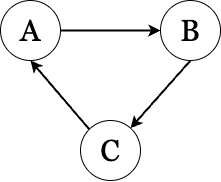
\includegraphics[width=0.6\textwidth,height=\textheight]{img/original_DCG.png}

}

\subcaption{\label{fig-examplegraphs-1}Example graph \(\mathcal{G}\)}

\end{minipage}%
%
\begin{minipage}{0.33\linewidth}

\centering{

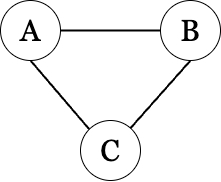
\includegraphics[width=0.6\textwidth,height=\textheight]{img/FCI_graph.png}

}

\subcaption{\label{fig-examplegraphs-2}Corresponding MAAG}

\end{minipage}%
%
\begin{minipage}{0.33\linewidth}

\centering{

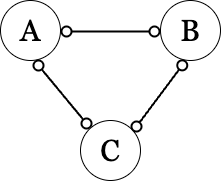
\includegraphics[width=0.6\textwidth,height=\textheight]{img/CCI_graph.png}

}

\subcaption{\label{fig-examplegraphs-3}Corrsponding PAG}

\end{minipage}%

\caption{\label{fig-examplegraphs}Example graph \(\mathcal{G}\)
featuring a cycle and the corresponding MAAG from CCI and PAG from FCI.}

\end{figure}%

The graph produced by the PC algorithm is a \emph{CPDAG} (completed
partially directed acyclic graph), where directed edges (\(A\) → \(B\))
indicate that \(A\) is a direct cause (parent) of \(B\). Unlike FCI and
CCI, the CPDAG does not include circle symbols. Instead, when the PC
algorithm cannot determine the direction of causality, it represents
this uncertainty with bidirectional arrows. While the PC algorithm
serves as a useful reference, its strict assumptions of acyclicity and
the absence of latent confounders restrict its applicability in more
complex scenarios. Therefore, our primary focus remains on the results
from FCI and CCI, with all PC algorithm results provided in the
\hyperref[sec-appendix]{Appendix} for completeness.

One practical challenge in applying these algorithms to the HELIUS
dataset is that the data does not follow a Gaussian distribution, and
the relationships among variables are unlikely to be strictly linear. To
account for this, we supplement the commonly used Gaussian conditional
independence (CI) test, which relies on partial correlations, with a
non-parametric CI test based on reproducing kernel methods (Zhang et
al., 2012). While kernel-based conditional independence tests (KCIT) are
effective, they are computationally intensive for large datasets like
HELIUS, as their quadratic scaling with sample size is primarily driven
by the inversion of large kernel matrices. To mitigate this issue, we
use the Randomized Conditional Correlation Test (RCoT), which
approximate kernel methods using random Fourier features. This approach
reduces computation to linear scaling with sample size, significantly
lowering computational costs (Strobl et al., 2019). For a more detailed
explanation of RCoT, refer to Section~\ref{sec-rcot}.

\subsection{Analysis}\label{analysis}

We analyze the causal structure using three approaches: examining the
relationship (1) between the five individual precarity factors and the
PHQ sum score, which represents overall depression severity; (2) between
individual symptoms and precarity factors; and (3) between individual
symptoms and overall precarity (the sum of the five precarity factors).
Using the PHQ sum score simplifies the analysis by reducing
dimensionality, offering computational efficiency and a broad,
interpretable perspective on the relationship between depression and
precarity factors. In contrast, analyzing individual symptoms provides a
more detailed understanding by capturing the diverse ways symptoms
respond to different precarity factors. However, this detailed approach
introduces methodological challenges, including non-standard
distributions of individual symptom variables and the complexities
associated with increased dimensionality. Finally, examining individual
symptoms in relation to the overall precarity score complements the
analysis by revealing how symptoms collectively connect to general
precarity. Aggregating precarity factors may uncover relationships that
could be overlooked in analyses of individual factors, particularly when
a symptom has associations across multiple factors that are not strong
enough to emerge in individual analyses. By integrating these three
approaches, we achieve a balance between capturing detailed granularity
and gaining a broader understanding of the relationship between
precarity and depression.

Furthermore, to address sensitivity to parameter values and enhance the
robustness of our results, we implement multiple settings combined with
bootstrapping. For each of the 100 bootstrap samples, we estimate causal
graphs and retain only the edges and directions that exceed predefined
thresholds. The analyses are conducted under the following conditions:

\begin{itemize}
\tightlist
\item
  Significance levels (\(\alpha\)): 0.01 and 0.05
\item
  Thresholds: 0.5, 0.6, 0.7, and 0.8
\item
  CI test: Gaussian CI test, RCoT
\item
  Algorithms: FCI, CCI, and PC
\end{itemize}

This setup yields 16 combinations (2 significance levels × 4 thresholds
× 2 CI tests), applied across three algorithms. Each combination is
repeated for 100 bootstrap samples, yielding a total of 1,600 graphs per
algorithm. For analyses involving individual symptom variables, we
simplify the setup by focusing on thresholds of 0.6 and 0.7 and reducing
the number of bootstrap samples to 30, easing computational demands. To
further enhance efficiency, we fix the skeleton of edges among symptom
variables based on the common structure estimated across all algorithms.
This approach minimizes spurious edges in the symptom network and
significantly reduces the computational time needed for skeleton
estimation. This fixed structure also aligns well with commonly reported
skeleton structures in the literature, ensuring consistency with
existing findings (\textbf{cite the comp\_model paper}).\footnote{We
  fixed the skeleton of the symptom network using a common structure
  derived from the PC, FCI, and CCI algorithms with an alpha level of
  0.001. This approach preserved the complexity of symptom interactions,
  enabling unrestricted estimation of causal directions both among
  symptoms (\emph{symptom --- symptom} interactions) and between
  symptoms and precarity factors.} Lastly, to summarize the results, we
identify the most frequently occurring edge endpoints across different
experimental setups.\footnote{The detailed proportion of each edge
  endpoint occurrence is provided in \textbf{?@sec-propmatrix}.} This
ensures that only stable and consistent edges are retained, providing a
clearer and more reliable understanding of the relationships between
precarity factors and depression. See Figure~\ref{fig-workflow} for an
overview of the analysis workflow.

\begin{figure}

\centering{

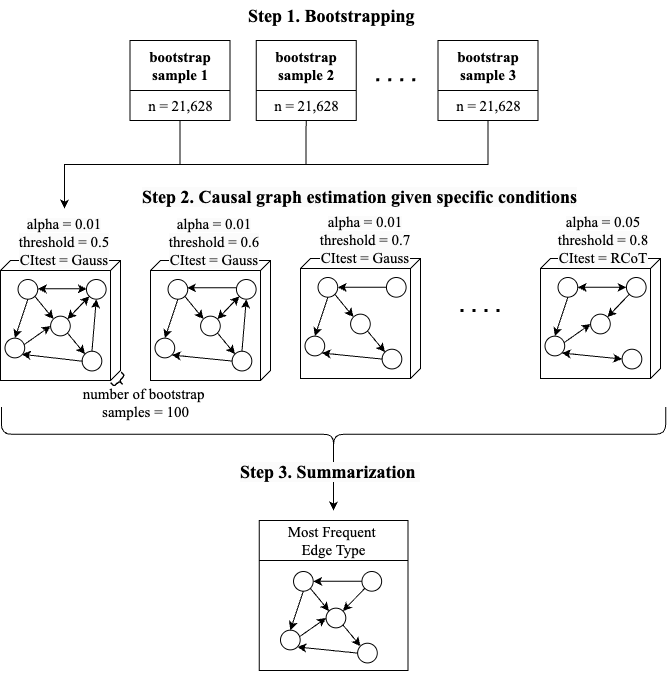
\includegraphics[width=0.8\textwidth,height=\textheight]{img/simsetup2.png}

}

\caption{\label{fig-workflow}Analysis workflow applied across all three
algorithms.}

\end{figure}%

\section{Results}\label{results}

\subsection{Depression as sum score}\label{depression-as-sum-score}

The sum score graphs provide a high-level summary of how precarity
factors collectively influence overall depression severity, focusing on
aggregated relationships. Figure~\ref{fig-sum} illustrates the causal
relationships between precarity factors (\emph{P.hou}, \emph{P.emp},
\emph{P.soc}, \emph{S.rel}, \emph{S.fin}) and the depression sum score
(\emph{PHQsum}) under two different setups: (a) using both Gaussian CI
test and RCoT, and (b) using RCoT alone. Black edges represent
consistent causal relationships identified by both FCI and CCI, while
gray dashed edges denote inconsistent relationships that vary between
the two methods. The inconsistent endpoints of the gray edges are marked
with circles.

In graph (a), the key pathways suggest that employment precarity
(\emph{P.emp}) and social precarity (\emph{P.soc}) do not cause
depression (\emph{PHQsum}). \emph{P.soc} does not cause recent
relational stress (\emph{S.rel}) or financial stress (\emph{S.fin}), and
these stressors are likely related by a latent confounder. Additionally,
\emph{P.emp} and \emph{S.fin} are identified as non-causes of housing
precarity (\emph{P.hou}). Both FCI and CCI detect a dependency between
\emph{P.emp} and \emph{S.fin}, but they disagree on the direction of the
relationship, leaving it unclear whether \emph{S.fin} causes
\emph{P.emp} or whether a latent confounder mediates their relationship.
Similar ambiguities are found in the connections between \emph{S.rel}
and \emph{PHQsum} and between \emph{S.fin} and \emph{PHQsum}.

Graph (b), derived solely from the nonparametric RCoT method. Both
graphs consistently identify that \emph{P.emp} is not a cause of
\emph{P.hou} or \emph{PHQsum}, and that \emph{P.soc} does not cause
\emph{PHQsum} or \emph{S.fin}. The relationship between stressors and
depression remains unresolved between the two algorithms. However, the
graph derived from RCoT provides greater confidence that depression is
not the cause of \emph{S.fin} and suggests a stronger likelihood that
the financial stress may contribute to depression or that their
relationship is mediated by a latent confounder. The role of relational
stress has become less pronounced, as the edge between \emph{P.soc} and
\emph{S.rel} is omitted, and the relationship between \emph{S.rel} and
\emph{S.fin} is now inconsistent between the algorithms.

Overall, both graphs together highlight the potential roles of stressors
like \emph{S.fin} and \emph{S.rel}, which are closely tied to
depression, either causally or via latent confounders. Employment and
social precarity may also be influenced by depression, either directly
or through latent variables. Lastly, housing precarity does not directly
impact depression but remains connected to employment precarity and
financial stress, likely mediated by direct or latent pathways.

\begin{figure}

\begin{minipage}{0.50\linewidth}

\centering{

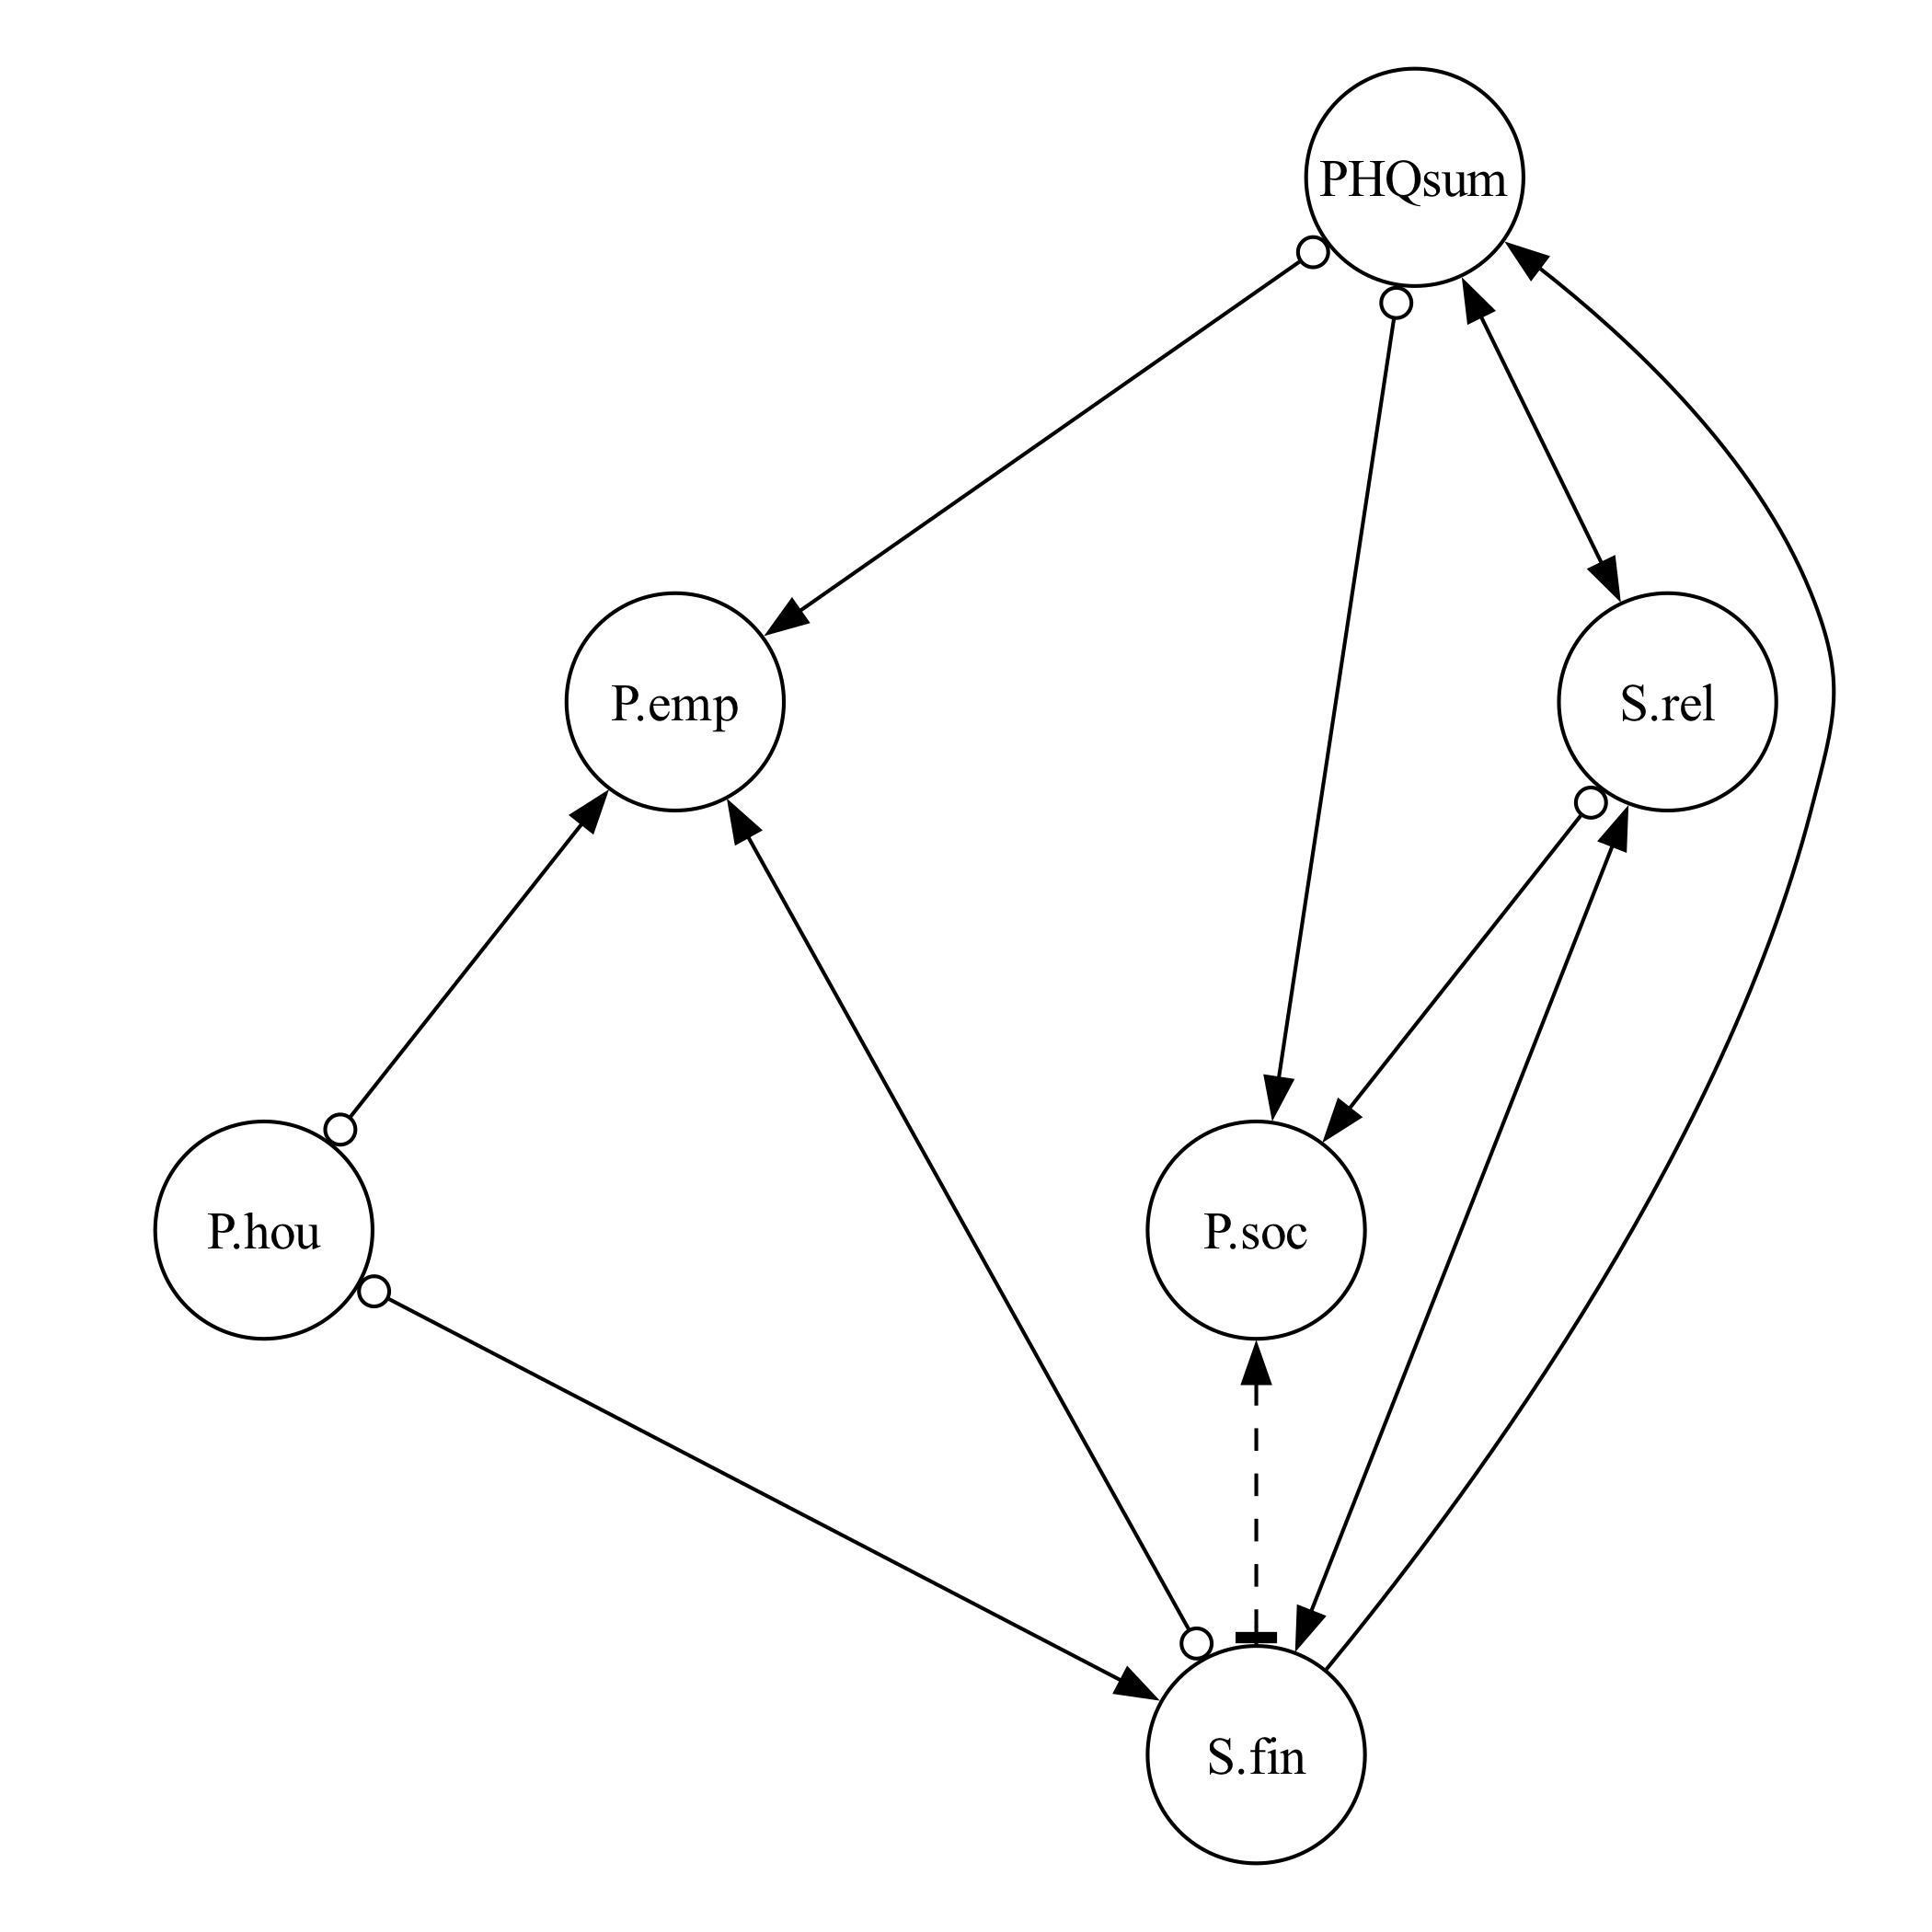
\includegraphics[width=1\textwidth,height=\textheight]{img/FCI_depsum.png}

}

\subcaption{\label{fig-sum-1}FCI PAG}

\end{minipage}%
%
\begin{minipage}{0.50\linewidth}

\centering{

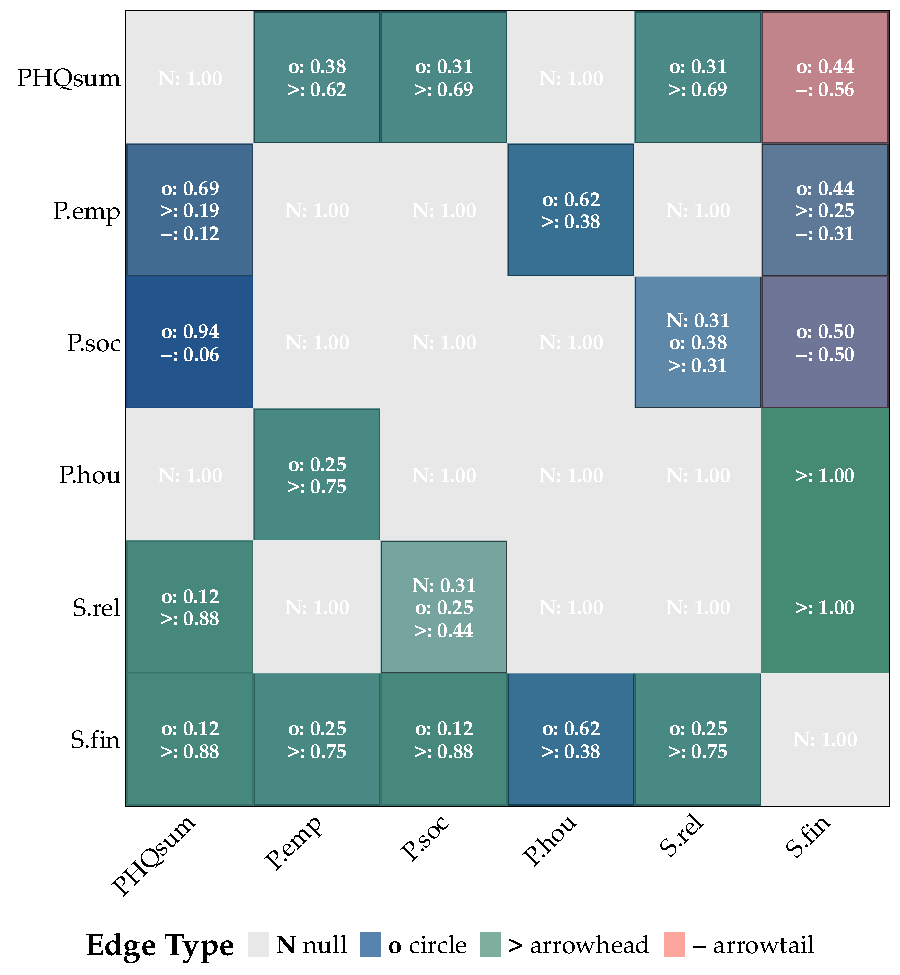
\includegraphics[width=1\textwidth,height=\textheight]{img/depsum_mat_fci.pdf}

}

\subcaption{\label{fig-sum-2}Proportion matrix}

\end{minipage}%

\caption{\label{fig-sum}Resulting graph of precarity factors and
depression sum score using FCI and proportion of edge endpoint types.}

\end{figure}%

\subsection{Individual depression
symptom}\label{individual-depression-symptom}

Moving from the sum score representation to the symptom-level graph
provides a more granular perspective on the causal relationships between
precarity factors and depression. This approach highlights the
heterogeneity in how precarity factors influence individual depressive
symptoms --- \emph{slp} (sleep), \emph{ene} (energy), \emph{app}
(appetite), \emph{mot} (motor), \emph{sui} (suicidal), \emph{anh}
(anhedonia), \emph{glt} (guilt), and \emph{dep} (depressed mood). While
the sum score graph aggregates all symptoms into a single
measure---potentially obscuring nuanced relationships---the symptom
graph uncovers distinct pathways for different symptoms. In the
symptom-level graph (Figure~\ref{fig-sym}), consistent relationships are
represented by black solid edges, while areas of disagreement between
the FCI and CCI algorithms are denoted by gray dashed edges. Endpoints
marked with circles indicate differences in directional conclusions
between the algorithms. Additionally, the navy dashed edges represent
relationships unique to the graphs generated using Gaussian CI testing.

The symptom-level graph reveals a complex and interconnected structure,
far more intricate than the sum score graph. Its denser network
highlights the strong interdependence among symptoms and suggests the
presence of latent confounding influences, as indicated by numerous
bidirectional arrows.

Certain nodes in the network emerge as more \emph{causally} central,
highlighting their potential importance as intervention points. Among
the depressive symptoms, \emph{anh}, \emph{dep}, \emph{slp}, and
\emph{glt} emerge as particularly influential, with multiple outgoing
edges (o-\textgreater) to other symptoms, suggesting their roles as
potential key drivers within the symptom network. Especially, symptoms
such as \emph{glt}, \emph{slp}, and \emph{anh} are particularly
critical, potentially acting as initiator or activator nodes within the
network due to their apparent connections with precarity factors. These
symptoms appear to be especially sensitive to external stressors,
potentially manifesting early in response to such conditions and
subsequently activating other interconnected symptom nodes.

The causal structure involving precarity factors in the symptom-level
graph is largely consistent with the patterns observed in the sum score
graphs. As in the sum graphs, relational stress (\emph{S.rel}) emerges
as a potential causal factor for depression, while employment
(\emph{P.emp}) and social precarity (\emph{P.soc}) are more likely to be
influenced by depressive symptoms. The symptom-level analysis, however,
provides more specificity by pinpointing the symptoms involved in these
relationships. For instance, \emph{slp} is identified as influencing
\emph{P.emp} or potentially through a latent confounder (\emph{slp}
o-\textgreater{} \emph{P.emp}) , while \emph{glt} appears to affect
\emph{P.soc} or may be linked via a confounder (\emph{glt}
o-\textgreater{} \emph{P.soc}). Additional edges are observed in the
graph generated using Gaussian CI tests, such as \emph{slp}
\textless-\textgreater{} \emph{S.rel} and \emph{slp} o-\textgreater{}
\emph{P.emp}. As seen in the sum graph, Gaussian CI testing tends to
produce a denser graph. In this case, causal relationships involving
\emph{slp} are particularly prominent.

Some discrepancies, however, exist between the symptom-level and sum
graphs. For example, financial stress (\emph{S.fin}) does not have any
edges with depressive symptoms in the symptom-level graph, although it
maintains associations with other precarity factors. Additionally,
housing precarity (\emph{P.hou}) becomes entirely disconnected from the
rest of the network, appearing as an isolated node.

\begin{figure}

\begin{minipage}{\linewidth}

\centering{

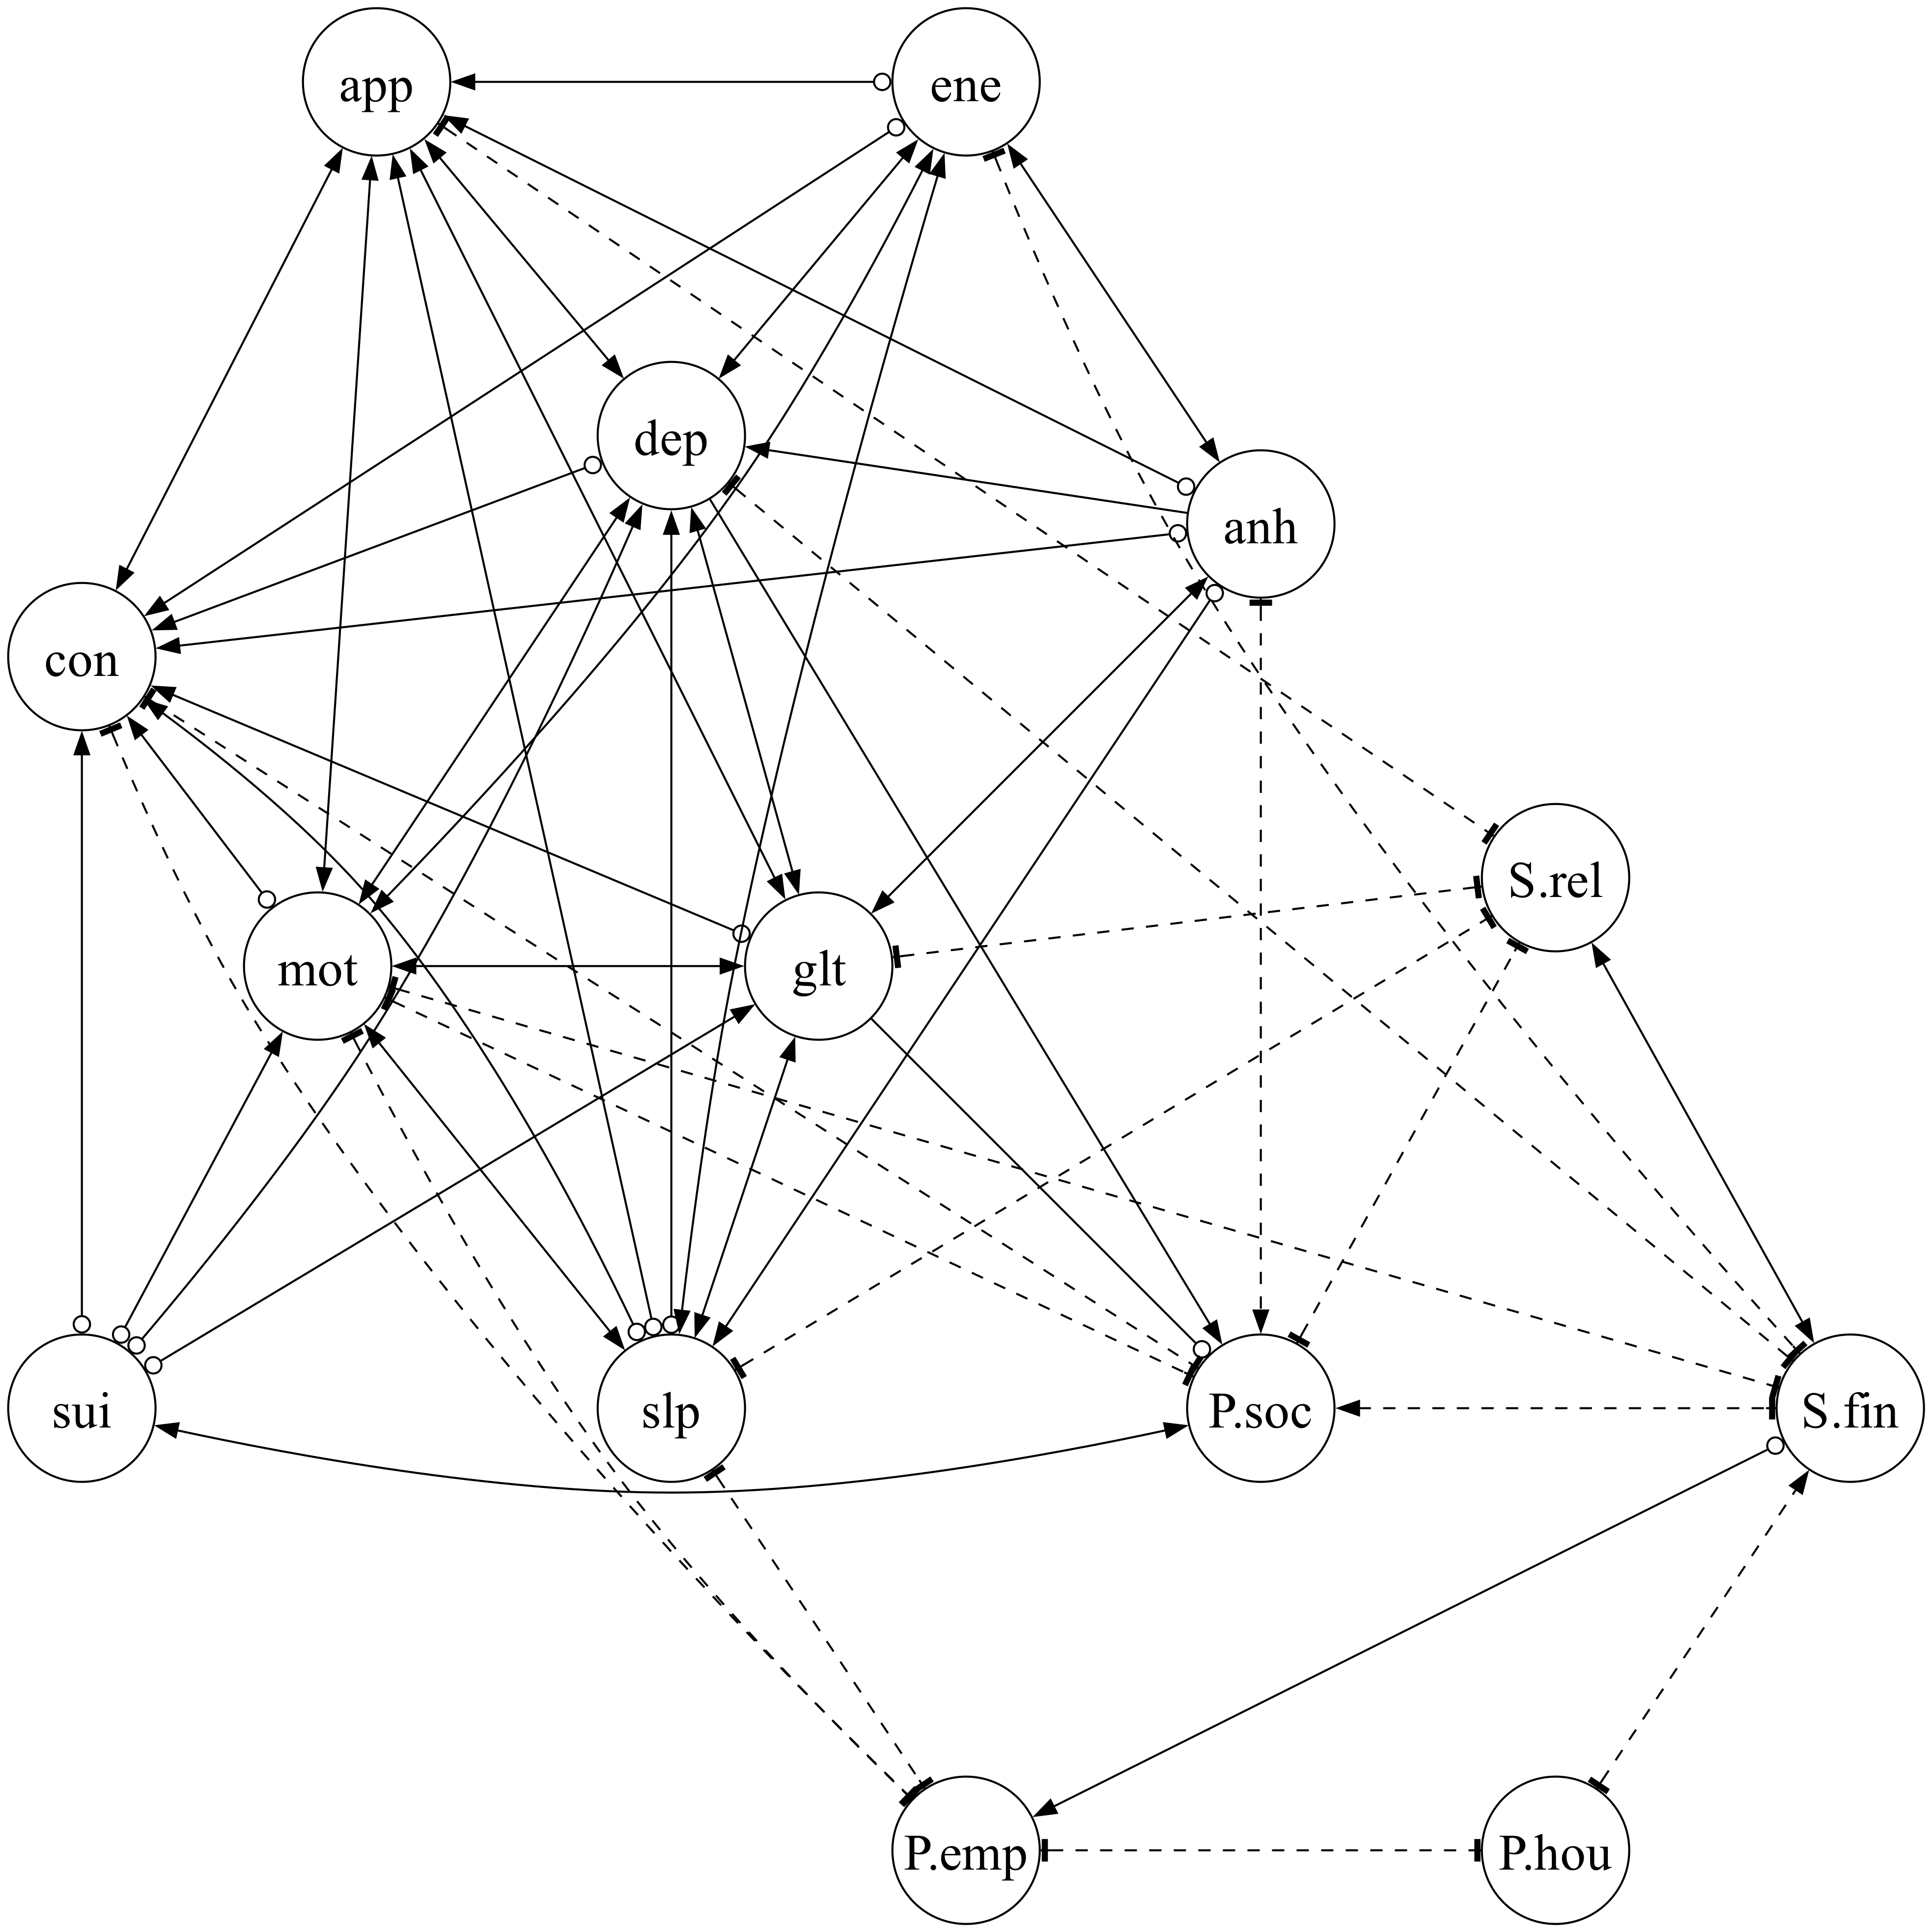
\includegraphics[width=0.7\textwidth,height=\textheight]{img/symptom_graph_FCI.png}

}

\subcaption{\label{fig-sym-1}FCI PAG}

\end{minipage}%
\newline
\begin{minipage}{\linewidth}

\centering{

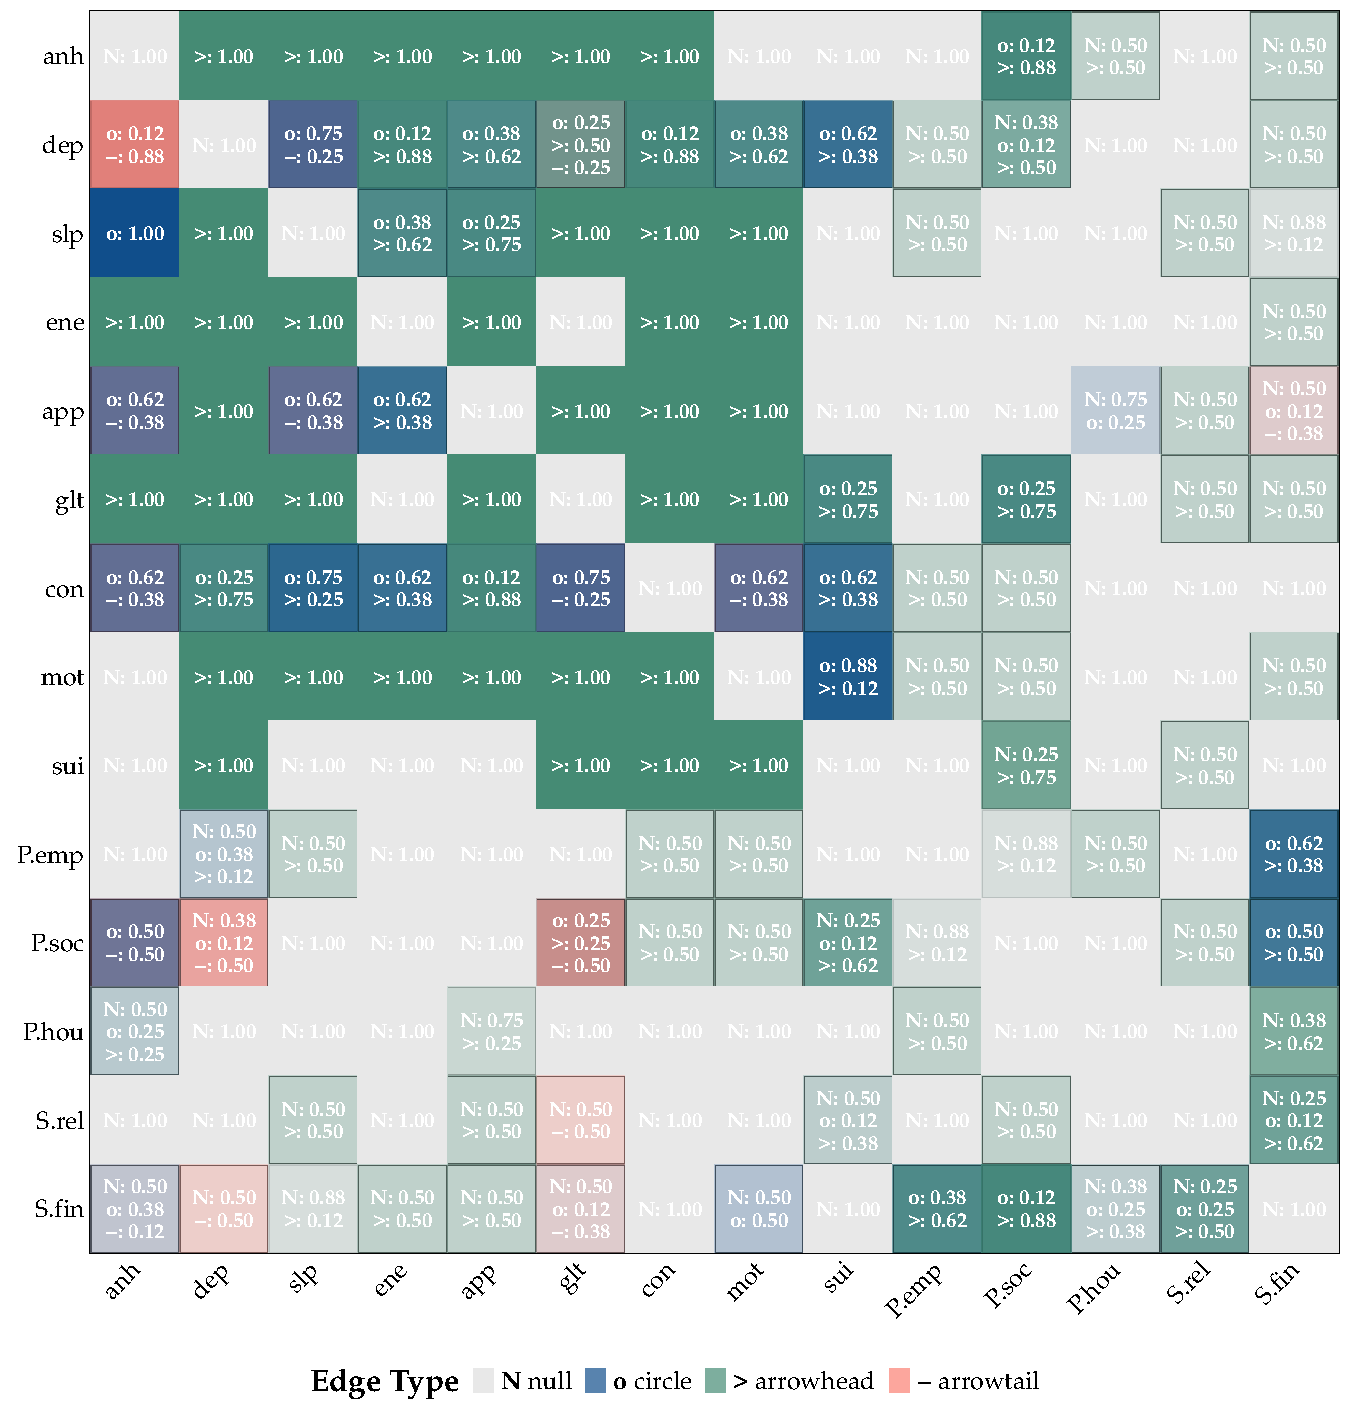
\includegraphics[width=0.7\textwidth,height=\textheight]{img/symptom_mat_fci.pdf}

}

\subcaption{\label{fig-sym-2}Proportion matrix}

\end{minipage}%

\caption{\label{fig-sym}Resulting graph of precarity factors and
individual depression symptoms using FCI and proportion of edge endpoint
types.}

\end{figure}%

\subsection{Precarity as sum score}\label{precarity-as-sum-score}

Lastly, we examine the relationships between individual symptoms and
overall precarity, represented as the sum of five precariousness
factors. This approach completes the analysis by providing a perspective
on how individual symptoms relate to overall precarity. It complements
the previous analysis, which focused on individual symptoms and
individual precarity factors, by potentially capturing distributed
relationships across different precarity factors through their
aggregation into a single overall score. As before, black solid lines
indicate edges agreed upon by both FCI and CCI, while gray dashed lines
represent edges where the two algorithms disagree. Circles at the
endpoints of gray dashed edges denote unresolved directionality.
Additionally, navy dashed edges highlight relationships that appear
exclusively in graphs generated using Gaussian CI tests.

Compared to Figure~\ref{fig-sym}, this analysis reveals greater
disagreement between FCI and CCI regarding edge directionality, as
evidenced by more dashed edges. FCI tends to estimate more undirected
edges (circles), while CCI more frequently assigns directed arrows
between symptom-symptom relationships. For a detailed breakdown, see
\textbf{?@sec-propmatrix}, which shows the proportion of symbols
produced by each algorithm. When examining overall precarity, we observe
that more symptoms are now connected to the precarity score
(\emph{Precarity}) compared to the individual precarity factor analysis
in Figure~\ref{fig-sym}. In addition to \emph{glt}, \emph{slp},
\emph{anh}, and \emph{sui}, which are previously shown to be connected
to individual precarity factors, \emph{mot}, \emph{app}, and \emph{dep}
are now identified as having causal relationships with overall
precarity. Furthermore, when using the Gaussian CI test, con is also
shown to be causally related to overall precarity. Notably, all these
connections are directed towards precarity (o→), indicating that overall
precarity is not the cause of symptoms. The exception is the
bidirectional edge between \emph{sui} \textless-\textgreater{}
\emph{Precarity}, which suggests a connection via latent confounders.
FCI predominantly estimates directed arrows (→) for symptom-precarity
relationships, suggesting that symptoms are driving precarity. With
fewer variables (reduced from 14 to 9), this approach appears to have
slightly more statistical power, enabling algorithms to estimate
relationships with greater confidence compared to the previous analysis
involving individual symptoms and individual precarity factors.

\begin{figure}

\begin{minipage}{\linewidth}

\centering{

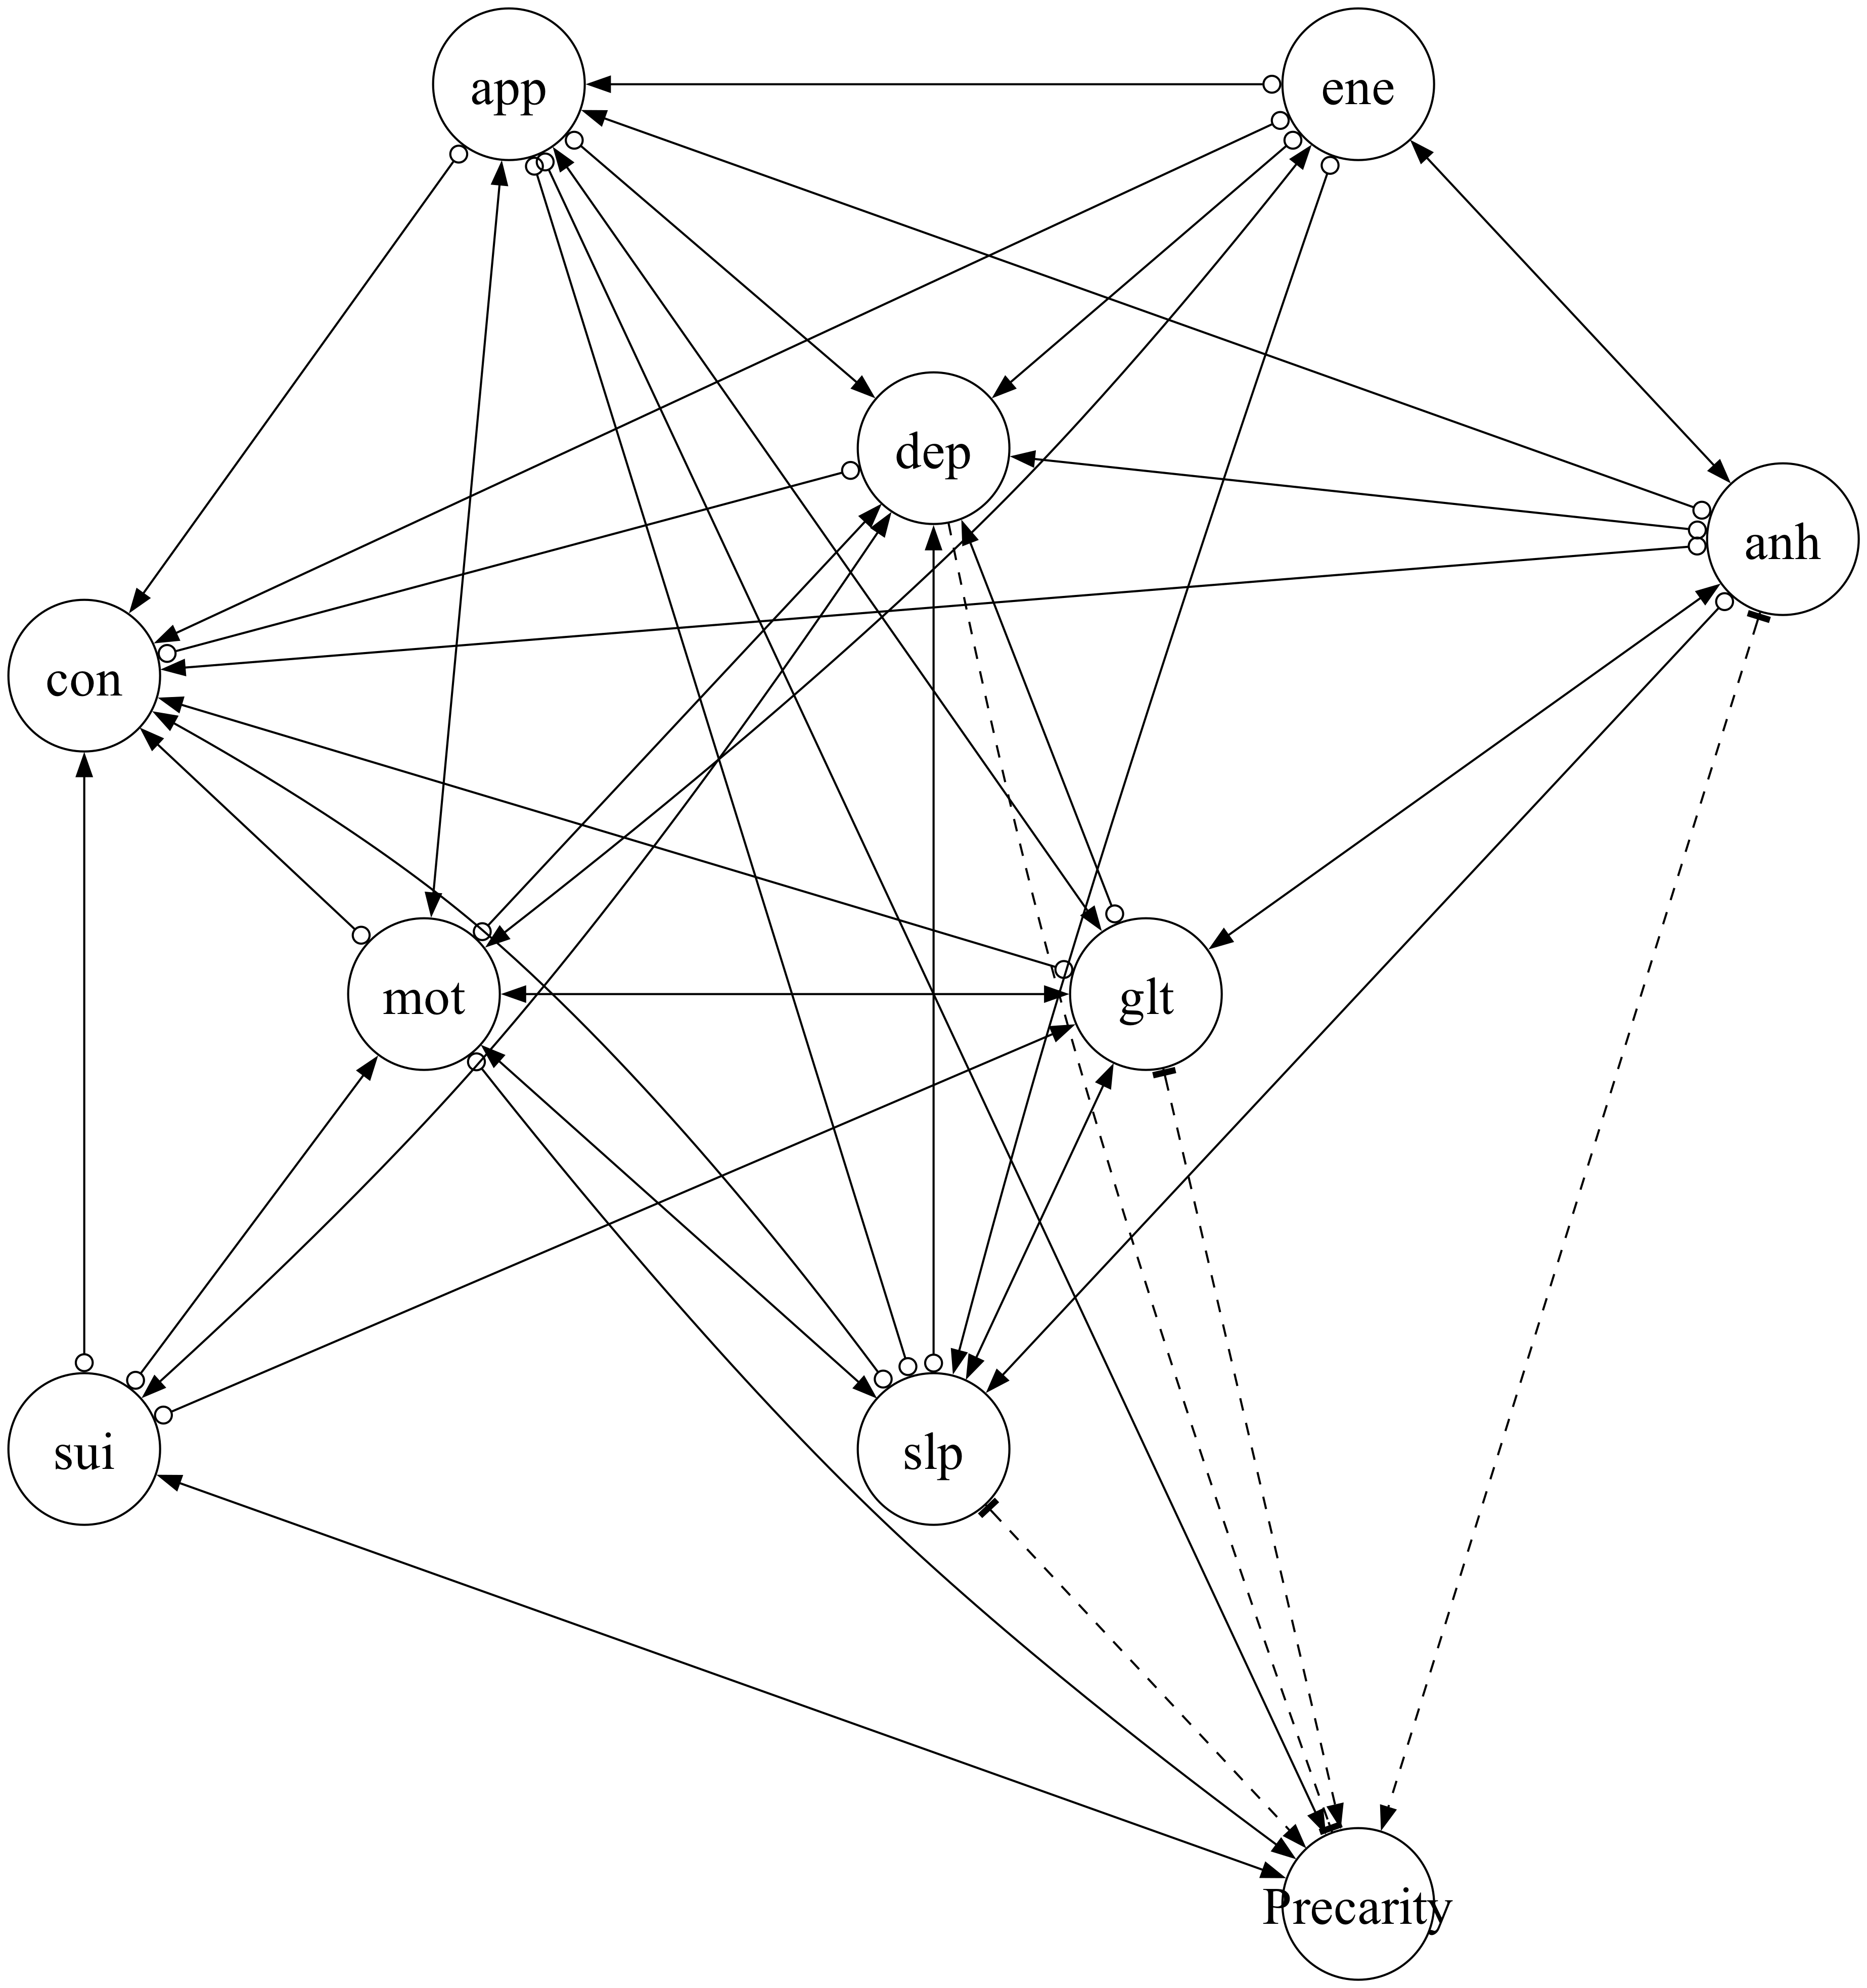
\includegraphics[width=0.6\textwidth,height=\textheight]{img/presum_graph_FCI.png}

}

\subcaption{\label{fig-presum-1}FCI PAG}

\end{minipage}%
\newline
\begin{minipage}{\linewidth}

\centering{

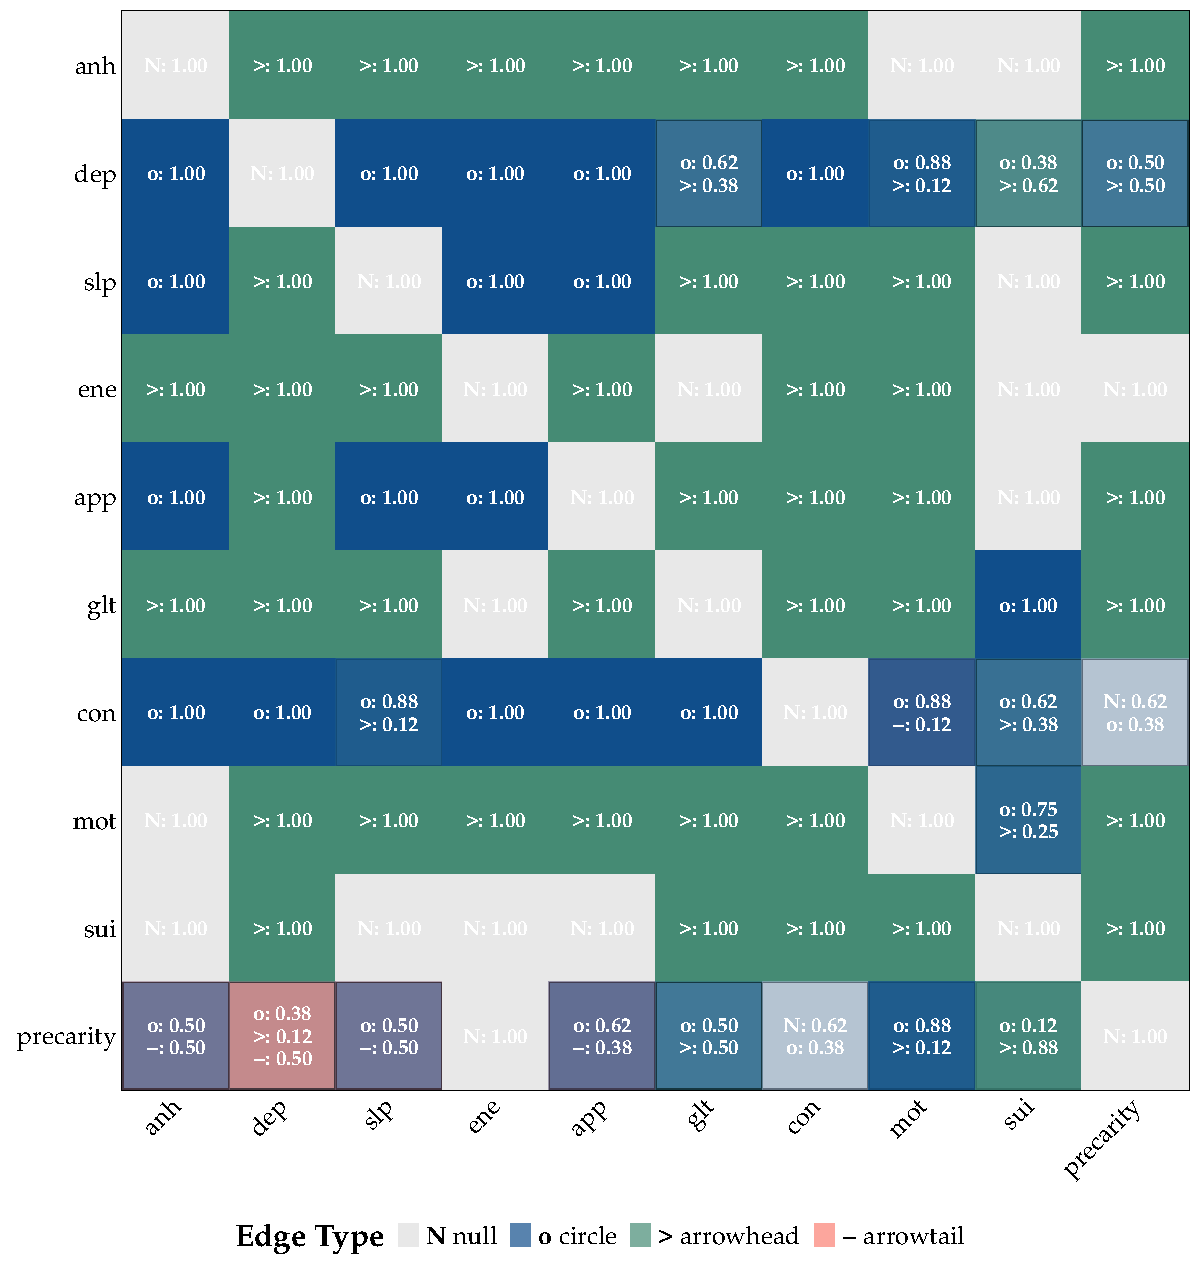
\includegraphics[width=0.6\textwidth,height=\textheight]{img/presum_mat_fci.pdf}

}

\subcaption{\label{fig-presum-2}Proportion matrix}

\end{minipage}%

\caption{\label{fig-presum}Resulting graph of precarity sum score and
individual depression symptoms using FCI and proportion of edge endpoint
types.}

\end{figure}%

\section{Discussion}\label{discussion}

The present study examined the causal relationships between precarity
factors and depression using causal discovery algorithms, incorporating
both sum score and symptom-level analyses. By analyzing PHQ sum scores
alongside individual symptom scores, and comparing aggregated precarity
scores with individual precarity factors, we gained a comprehensive
perspective on how different aspects of precarity influence depression.
This dual approach highlighted nuanced pathways that may be overlooked
when focusing solely on aggregate measures, while also capturing broader
interactions that might remain undetected in analyses limited to
individual factors.

Our findings highlight the significant role of recent relational stress
(\emph{S.rel}) as a potential causal factor for depression, consistently
observed across both sum score and symptom-level analyses. This
consistency underscores the profound impact interpersonal relationships
can have on mental health. The symptom-level analysis further identified
specific symptoms, such as sleep disturbances (\emph{slp}), guilt
(\emph{glt}), and anhedonia (\emph{anh}), as particularly sensitive to
external precarity conditions. These symptoms emerged as potential
initiators or activators within the depressive symptom network,
suggesting that they may serve as early warning signs or valuable
targets for preventive interventions.

Employment precarity (\emph{P.emp}) and social precarity (\emph{P.soc})
were more likely to be influenced by depressive symptoms rather than
acting as direct causes. The symptom-level graph provided additional
clarity by identifying that sleep disturbances influenced employment
precarity (\emph{slp} o-\textgreater{} \emph{P.emp}) and feelings of
guilt affected social precarity (\emph{glt} o-\textgreater{}
\emph{P.soc}). This directional insight suggests that interventions
targeting specific depressive symptoms may have downstream effects on
improving certain aspects of precarity.

Interestingly, financial stress (\emph{S.fin}) did not exhibit causal
relationships with individual depressive symptoms in the symptom-level
analysis, contrasting with its apparent role in the sum score graphs.
This divergence indicates that while financial stress may influence
overall depression severity, its impact on specific symptoms may not be
significant. Also, housing precarity (\emph{P.hou}) emerged as an
isolated node in the symptom-level graph, losing all connections with
other precarity factors. This isolation suggests that housing precarity
may operate independently of the depressive symptom network or that its
effects are not captured within the scope of the measured variables.

Several limitations should be acknowledged when interpreting these
findings. The prevalence of bidirectional arrows and circle-marked
endpoints in the graphs reflects unresolved ambiguities in the causal
relationships suggested by the data. These uncertainties highlight the
need for further research, particularly with higher-resolution datasets,
such as time-series data. Incorporating time-series data could capture
temporal dynamics between precarity factors and depressive symptoms,
providing time-specific insights and revealing how these relationships
evolve over time. Methods like \emph{PCMCI} (Runge et al., 2019),
\emph{tsFCI} (Entner \& Hoyer, 2010), and other time-series adaptations
of causal discovery algorithms could offer a more robust framework for
addressing temporal dependencies and refining the analysis.

Another notable limitation is the absence of clear evidence for cycles
within the symptom network, despite employing algorithms designed to
account for cyclic relationships. The CCI algorithm primarily produced
bidirectional arrows, while FCI predominantly generated directional
arrows, yet neither demonstrated patterns indicative of definitive
cyclic structures. This suggests that addressing cyclic relationships is
particularly challenging when relying solely on observational datasets.
Future research could benefit from refined datasets that incorporate
intervention data. Methods such as \emph{LLC} (Hyttinen et al., 2012),
\emph{NODGAS-Flow }(Sethuraman et al., 2023), and the recently developed
\emph{Bicycle} algorithm (Rohbeck et al., 2024), which utilize both
observational and intervention data, may uncover potential cycles more
effectively.

Lastly, regarding conditional independence (CI) testing, the differences
between the graphs generated by Gaussian CI and RCoT underscore the
methodological sensitivities in detecting causal relationships. Gaussian
CI produced denser graphs, which is somewhat counterintuitive, as the
Gaussian CI's strict linearity assumption would typically result in
fewer detected relationships, not more. A possible explanation for this
discrepancy is that Gaussian CI's reliance on partial correlations may
overestimate relationships when specific non-linear dependencies exist
in the data. In contrast, RCoT, free from such assumptions, might better
capture independence patterns under such conditions. However, RCoT is
not without its limitations. While technically non-parametric, its
performance can be influenced by the distributional characteristics of
the data. The Gaussian RBF (radial basis function) kernel, optimized for
continuous data with smooth transitions, may struggle with discrete or
mixed datasets, where distances between discrete points may fail to
convey meaningful similarity (Howlett, 2001). This limitation could
explain why RCoT might miss certain dependencies, particularly in the
HELIUS dataset, where some variables lack smooth continuity. Future
research could tackle these challenges by developing hybrid kernels
designed for mixed datasets, integrating both continuous and discrete
variables into RCoT-like methods. This would have the potential to
improve the reliability of findings, especially when working with
datasets characterized by complex and heterogeneous structures.

Despite its limitations, this study marks a meaningful step toward
understanding the mechanisms linking precarity factors and depression.
By applying causal discovery methods, it moves beyond traditional
association-based analyses, providing insights that can inform more
precise and targeted interventions. While the resulting graphs are
preliminary and contain unresolved ambiguities, they offer a valuable
starting point for leveraging causal discovery tools to investigate the
causal interplay between depression and precarity factors. A promising
next step would involve integrating these causal structures into
computational models, such as the symptom dynamic model proposed in
\textbf{our comp-model paper}. By simulating intervention effects, such
models could provide more realistic insights into how targeted actions
might influence symptom networks and precarity factors over time. For
example, interventions focused on improving sleep hygiene or alleviating
guilt could be evaluated for their cascading effects on employment and
social relationships, offering actionable guidance for designing
population-level mental health strategies. As one of the early
applications of causal discovery tools to the complex dynamics of
depression and precarity factors, this study lays a foundation for
future research. We hope it inspires further refinement of these methods
and ultimately contribute to more effective solutions for alleviating
depression and improving societal well-being.

\section{References}\label{references}

\phantomsection\label{refs}
\begin{CSLReferences}{1}{0}
\bibitem[\citeproctext]{ref-dojer2016learning}
Dojer, N. (2016). Learning bayesian networks from datasets joining
continuous and discrete variables. \emph{International Journal of
Approximate Reasoning}, \emph{78}, 116--124.

\bibitem[\citeproctext]{ref-entner2010causal}
Entner, D., \& Hoyer, P. O. (2010). On causal discovery from time series
data using FCI. \emph{Probabilistic Graphical Models}, \emph{16}.

\bibitem[\citeproctext]{ref-forre2018constraint}
Forré, P., \& Mooij, J. M. (2018). Constraint-based causal discovery for
non-linear structural causal models with cycles and latent confounders.
\emph{arXiv Preprint arXiv:1807.03024}.

\bibitem[\citeproctext]{ref-howlett2001radial}
Howlett, R. J. (2001). \emph{Radial basis function networks 1: Recent
developments in theory and applications}.

\bibitem[\citeproctext]{ref-hyttinen2012learning}
Hyttinen, A., Eberhardt, F., \& Hoyer, P. O. (2012). Learning linear
cyclic causal models with latent variables. \emph{The Journal of Machine
Learning Research}, \emph{13}(1), 3387--3439.

\bibitem[\citeproctext]{ref-lindsay2000moment}
Lindsay, B. G., Pilla, R. S., \& Basak, P. (2000). Moment-based
approximations of distributions using mixtures: Theory and applications.
\emph{Annals of the Institute of Statistical Mathematics}, \emph{52},
215--230.

\bibitem[\citeproctext]{ref-mooij2020constraint}
Mooij, J. M., \& Claassen, T. (2020). Constraint-based causal discovery
using partial ancestral graphs in the presence of cycles.
\emph{Conference on Uncertainty in Artificial Intelligence}, 1159--1168.

\bibitem[\citeproctext]{ref-neapolitan2004learning}
Neapolitan, R. E. et al. (2004). \emph{Learning bayesian networks} (Vol.
38). Pearson Prentice Hall Upper Saddle River.

\bibitem[\citeproctext]{ref-park2024discovering}
Park, K., Waldorp, L. J., \& Ryan, O. (2024). Discovering cyclic causal
models in psychological research. \emph{Advances. In/Psychology},
\emph{2}, e72425.

\bibitem[\citeproctext]{ref-rohbeck2024}
Rohbeck, M., Clarke, B., Mikulik, K., Pettet, A., Stegle, O., \&
Ueltzhöffer, K. (2024). Bicycle: Intervention-based causal discovery
with cycles. In F. Locatello \& V. Didelez (Eds.), \emph{Proceedings of
the third conference on causal learning and reasoning} (Vol. 236, pp.
209--242). PMLR.
\url{https://proceedings.mlr.press/v236/rohbeck24a.html}

\bibitem[\citeproctext]{ref-runge2019detecting}
Runge, J., Nowack, P., Kretschmer, M., Flaxman, S., \& Sejdinovic, D.
(2019). Detecting and quantifying causal associations in large nonlinear
time series datasets. \emph{Science Advances}, \emph{5}(11), eaau4996.

\bibitem[\citeproctext]{ref-sethuraman2023nodags}
Sethuraman, M. G., Lopez, R., Mohan, R., Fekri, F., Biancalani, T., \&
Hütter, J.-C. (2023). NODAGS-flow: Nonlinear cyclic causal structure
learning. \emph{International Conference on Artificial Intelligence and
Statistics}, 6371--6387.

\bibitem[\citeproctext]{ref-snijder2017cohort}
Snijder, M. B., Galenkamp, H., Prins, M., Derks, E. M., Peters, R. J.,
Zwinderman, A. H., \& Stronks, K. (2017). Cohort profile: The healthy
life in an urban setting (HELIUS) study in amsterdam, the netherlands.
\emph{BMJ Open}, \emph{7}(12), e017873.

\bibitem[\citeproctext]{ref-spirtes2001causation}
Spirtes, P., Glymour, C., \& Scheines, R. (2001). \emph{Causation,
prediction, and search}. MIT press.

\bibitem[\citeproctext]{ref-spirtes_causal_1995}
Spirtes, P., Meek, C., \& Richardson, T. (1995). Causal inference in the
presence of latent variables and selection bias. \emph{Proceedings of
the {Eleventh} Conference on {Uncertainty} in Artificial Intelligence},
499--506.

\bibitem[\citeproctext]{ref-strobl2019}
Strobl, E. V. (2019). A constraint-based algorithm for causal discovery
with cycles, latent variables and selection bias. \emph{International
Journal of Data Science and Analytics}, \emph{8}(1), 33--56.
\url{https://doi.org/10.1007/s41060-018-0158-2}

\bibitem[\citeproctext]{ref-strobl2019approximate}
Strobl, E. V., Zhang, K., \& Visweswaran, S. (2019). Approximate
kernel-based conditional independence tests for fast non-parametric
causal discovery. \emph{Journal of Causal Inference}, \emph{7}(1),
20180017.

\bibitem[\citeproctext]{ref-zhang2012kernel}
Zhang, K., Peters, J., Janzing, D., \& Schölkopf, B. (2012).
Kernel-based conditional independence test and application in causal
discovery. \emph{arXiv Preprint arXiv:1202.3775}.

\end{CSLReferences}

\section{Appendix}\label{sec-appendix}

\subsection{Precariousness factors by
Leonie}\label{precariousness-factors-by-leonie}

\begin{enumerate}
\def\labelenumi{\arabic{enumi}.}
\tightlist
\item
  EMPLOYMENT PRECARIOUSNESS
\end{enumerate}

\begin{itemize}
\tightlist
\item
  \texttt{H1\_Arbeidsparticipatie}: Working status
\item
  \texttt{H1\_WerkSit}: Which work situation most applies to you?
\item
  \texttt{H1\_RecentErv8}: Experiences past 12 months: h. You were
  sacked from your job or became unemployed (\emph{reverse})
\end{itemize}

\begin{enumerate}
\def\labelenumi{\arabic{enumi}.}
\setcounter{enumi}{1}
\tightlist
\item
  FINANCIAL PRECARIOUSNESS
\end{enumerate}

\begin{itemize}
\tightlist
\item
  \texttt{H1\_InkHhMoeite}: During the past year, did you have problems
  managing your household income?
\item
  \texttt{H1\_RecentErv9}: Experiences past 12 months: i. You had a
  major financial crisis (\emph{reverse})
\end{itemize}

\begin{enumerate}
\def\labelenumi{\arabic{enumi}.}
\setcounter{enumi}{2}
\tightlist
\item
  HOUSING PRECARIOUSNESS
\end{enumerate}

\begin{itemize}
\tightlist
\item
  \texttt{veilig\_2012}: Score safety (veiligheid) in 2012
  (\emph{reverse})
\item
  \texttt{vrz\_2012}: Score level of resources (niveau voorzieningen) in
  2012 (\emph{reverse})
\item
  \texttt{P\_HUURWON}: Percentage Huurwoningen
\end{itemize}

\begin{enumerate}
\def\labelenumi{\arabic{enumi}.}
\setcounter{enumi}{3}
\tightlist
\item
  CULTURAL PRECARIOUSNESS
\end{enumerate}

\begin{itemize}
\tightlist
\item
  \texttt{H1\_Discr\_sumscore}: Perceived discrimination: sum score of 9
  items (range 9-45)
\item
  \texttt{H1\_SBSQ\_meanscore}: Health literacy: SBSQ meanscore (range
  1-5) (\emph{reverse})
\item
  \texttt{A\_BED\_RU}: Aantal bedrijfsvestigingen; cultuur, recreatie,
  overige diensten (\emph{reverse})
\end{itemize}

\begin{enumerate}
\def\labelenumi{\arabic{enumi}.}
\setcounter{enumi}{4}
\tightlist
\item
  SOCIAL PRECARIOUSNESS
\end{enumerate}

\begin{itemize}
\tightlist
\item
  \texttt{H1\_RecentErv5}: Experiences past 12 months: e. Your steady
  relationship ended (\emph{reverse})
\item
  \texttt{H1\_RecentErv6}: Experiences past 12 months: f.~A long-term
  friendship with a good friend or family member was broken off
  (\emph{reverse})
\item
  \texttt{H1\_RecentErv7}: Experiences past 12 months: g. You had a
  serious problem with a good friend or family member, or neighbour
  (\emph{reverse})
\item
  \texttt{H1\_SSQT}: SSQT (frequency of social contact): sum score of 5
  items (range 5-20) (\emph{reverse})
\item
  \texttt{H1\_SSQSa}: SSQS (adequacy of social contact): sum score of 5
  items, category 3 and 4 not combined (range 5-20) (\emph{reverse})
\end{itemize}

\begin{center}
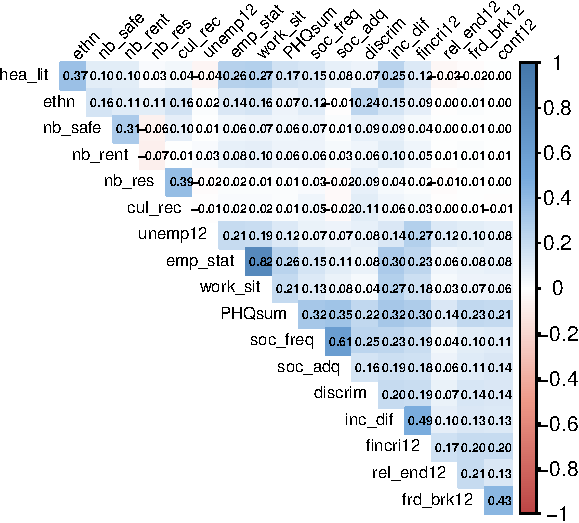
\includegraphics{draft_v1_files/figure-pdf/unnamed-chunk-9-1.pdf}
\end{center}

\begin{itemize}
\item
  \textbf{High} Correlations: \texttt{emp\_stat} (employment status) and
  \texttt{work\_sit} (work situation) have a strong positive correlation
  of 0.82. This suggests that individuals with higher employment status
  tend to have more secure or favorable work situations.
  \texttt{soc\_freq} (social contact frequency) shows a strong positive
  correlation with \texttt{soc\_adq} (social adequacy) at 0.61. This
  indicates that individuals with more frequent social contact also tend
  to have higher perceived adequacy of social interactions.
\item
  \textbf{Moderate} Correlations: \texttt{nb\_safe} (neighborhood
  safety) and \texttt{nb\_res} (resources) have a moderate positive
  correlation of 0.39, suggesting that areas with higher safety also
  have better resources. \texttt{hea\_lit} (health literacy) has
  moderate correlations with \texttt{emp\_stat} (0.26) and
  \texttt{work\_sit} (0.25), which could mean that higher health
  literacy is associated with better employment situations.
  \texttt{frd\_brk12} (friendship breakups) and \texttt{conf12}
  (conflicts) have a notable correlation of 0.43, indicating a
  relationship between having conflicts and friendship losses.
\item
  \textbf{Low to Moderate} Correlations in Financial Precariousness:
  \texttt{inc\_dif} (income difficulties) has a moderate correlation
  with \texttt{fincri12} (financial crisis) at 0.49. This aligns with
  the expected relationship, where individuals who experience general
  income difficulties are more likely to report financial crises.
\item
  \textbf{Low} Correlations (0.1 - 0.2): Many variables, such as
  \texttt{discrim} (discrimination), \texttt{unemp12} (unemployment
  experience), and \texttt{rel\_end12} (relationship end), have low
  correlations with other variables, suggesting relatively independent
  relationships in the context of this dataset.
\end{itemize}

\subsection{Exploratory Factor Analysis
(EFA)}\label{exploratory-factor-analysis-efa}

\begin{center}
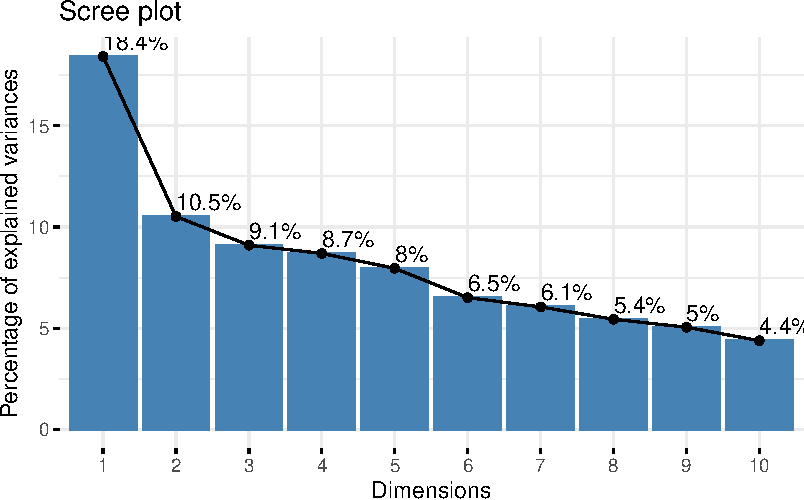
\includegraphics[width=0.55\textwidth,height=\textheight]{draft_v1_files/figure-pdf/unnamed-chunk-10-1.pdf}
\end{center}

\begin{center}
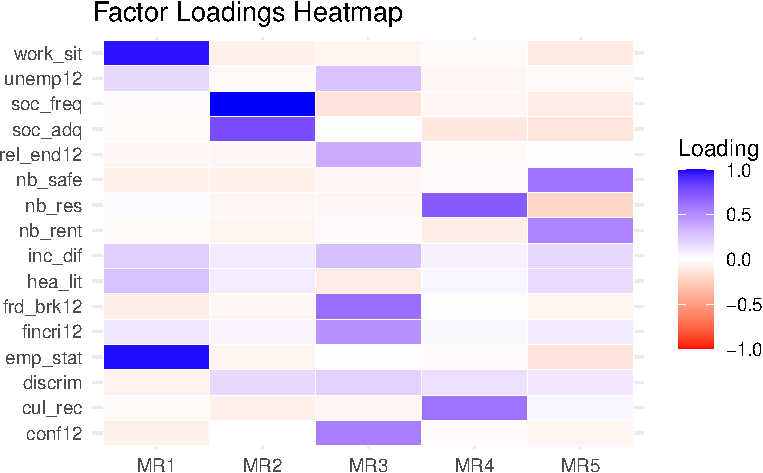
\includegraphics[width=0.7\textwidth,height=\textheight]{draft_v1_files/figure-pdf/unnamed-chunk-11-1.pdf}
\end{center}

\subsubsection{Factor Loadings (Pattern
Matrix)}\label{factor-loadings-pattern-matrix}

\begin{itemize}
\tightlist
\item
  \textbf{MR1}: High loadings on \texttt{emp\_stat} and
  \texttt{work\_sit} suggest this factor captures \emph{employment}
  precariousness.
\item
  \textbf{MR2}: Strong loadings on \texttt{soc\_freq} and
  \texttt{soc\_adq} indicate \emph{social} precariousness.
\item
  \textbf{MR3}: Key items like \texttt{frd\_brk12}, \texttt{conf12}, and
  \texttt{fincri12}, suggest recent \emph{stressful events}.
\item
  \textbf{MR4}: High loadings on \texttt{nb\_res} and \texttt{cul\_rec}
  may reflect \emph{community resources} precariousness.
\item
  \textbf{MR5}: Variables \texttt{nb\_safe} and \texttt{nb\_rent} with
  high loadings indicate \emph{housing} precariousness.
\end{itemize}

\subsubsection{Variance Explained}\label{variance-explained}

The factors cumulatively explain \textbf{38\%} of the variance, with MR1
being the most influential factor. Each factor contributes a smaller
proportion to the total variance (MR1 at 12\%, MR2 at 9\%, etc.).

\subsubsection{Factor Intercorrelations}\label{factor-intercorrelations}

Factors are moderately correlated, especially between \emph{MR1 and
MR5}, and \emph{MR2 and MR3}. This indicates that while distinct, these
factors are related---reasonable in a complex socio-economic context.

\subsubsection{Model Fit Statistics}\label{model-fit-statistics}

RMSEA (0.071) suggest an acceptable fit. Tucker Lewis Index (0.802)
suggests moderate reliability for the model.

\subsubsection{Summary}\label{summary}

The 5-factor model appears interpretable and captures distinct
dimensions of precariousness: \emph{employment, social, stressors,
community resources, and housing precariousness}. Although the overall
fit and explained variance could be stronger, these factors offer
insights into the underlying structure of the data, highlighting key
areas of precariousness.

\subsection{PCA}\label{pca}

\begin{center}
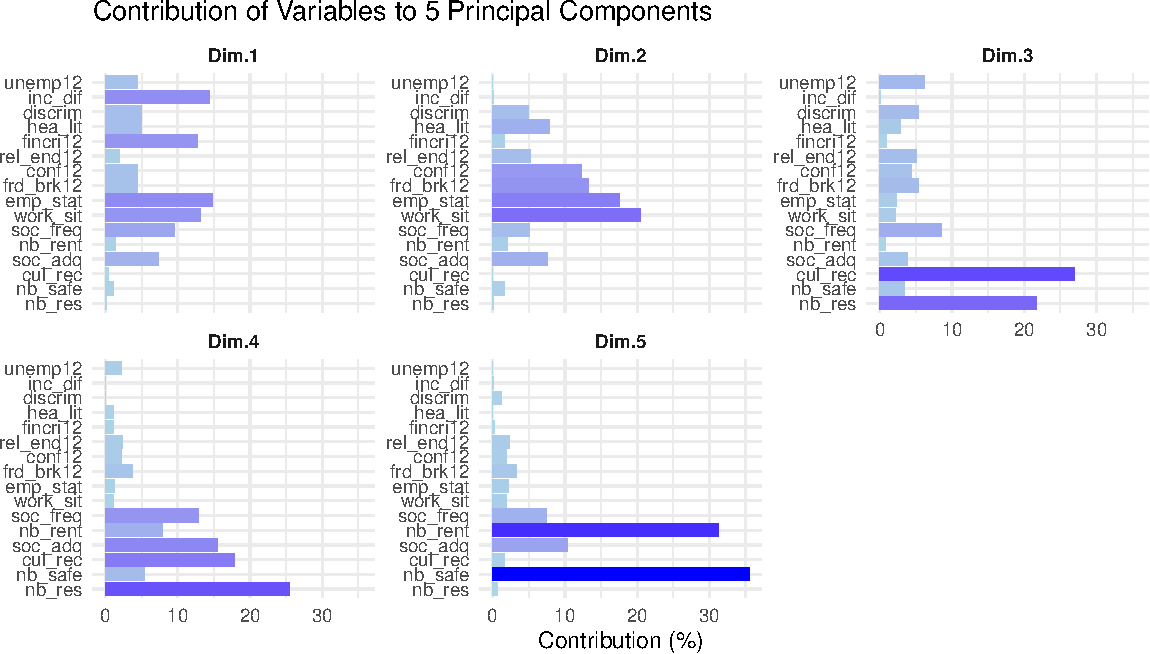
\includegraphics[width=0.7\textwidth,height=\textheight]{draft_v1_files/figure-pdf/unnamed-chunk-12-1.pdf}
\end{center}

\begin{itemize}
\tightlist
\item
  Component Retention: The scree plot shows a clear ``elbow'' after the
  first component. This steep drop suggests that most variance is
  explained by the first component. After Dimension 5, the percentage of
  explained variance decreases slightly more gradually, indicating
  diminishing returns for adding more components. If we need to choose
  multiple components, retaining the first 5 components seems
  reasonable, as they capture most of the variance (cumulatively
  explaining about 54.7\% of the total variance).
\end{itemize}

\begin{center}
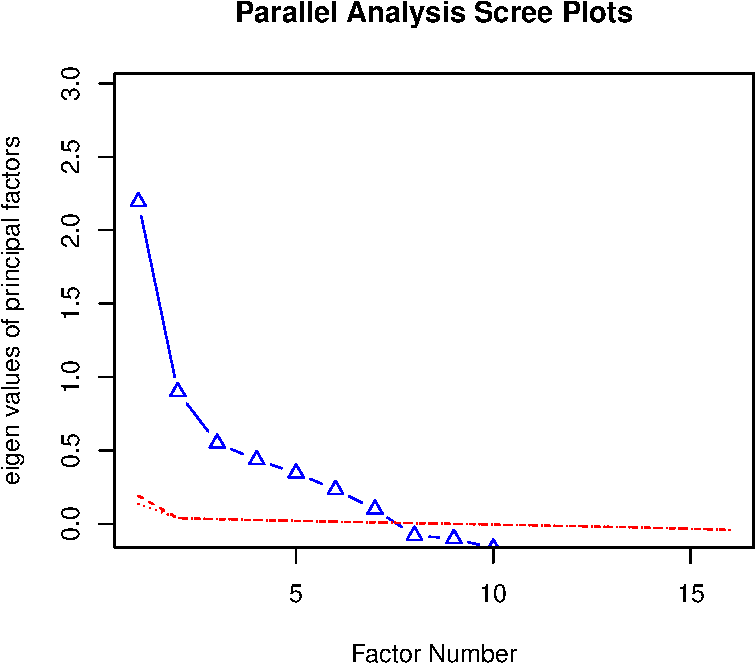
\includegraphics{draft_v1_files/figure-pdf/unnamed-chunk-13-1.pdf}
\end{center}

\subsubsection{Explained variance (contributions) of
variables}\label{explained-variance-contributions-of-variables}

It shows the importance of variables within each component.

\begin{itemize}
\item
  \textbf{Dim1}: High contributions are observed from
  \texttt{emp\_stat}, \texttt{work\_sit}, \texttt{inc\_dif}, and
  \texttt{fincri12}, suggesting that this dimension captures aspects of
  \emph{employment and financial} security.
\item
  \textbf{Dim2}: While \texttt{emp\_stat} and \texttt{work\_sit} overlap
  with Dim1, the strong contributions from \texttt{frd\_brk12} and
  \texttt{rel\_end12} indicate that this dimension captures a focus on
  \emph{recent relationship stressors}.
\item
  \textbf{Dim3}: \texttt{cul\_rec}, \texttt{nb\_res} have the highest
  contributions, indicating this dimension likely represents
  \emph{community and cultural} factors.
\item
  \textbf{Dim4}: \texttt{soc\_freq} and \texttt{soc\_adq} stand out in
  this dimension, suggesting an emphasis on \emph{social}
  precariousness.
\item
  \textbf{Dim5}: \texttt{nb\_safe} and \texttt{nb\_rent} are the top
  contributors, pointing to \emph{housing} security as key themes in
  this component.
\end{itemize}

\subsubsection{Cos² Values}\label{cosuxb2-values}

Cos² (squared cosine) values, or the quality of representation, show how
well each variable is represented by each dimension. where higher cos²
values (closer to 1) indicate better representation of a variable by a
component.

\begin{center}
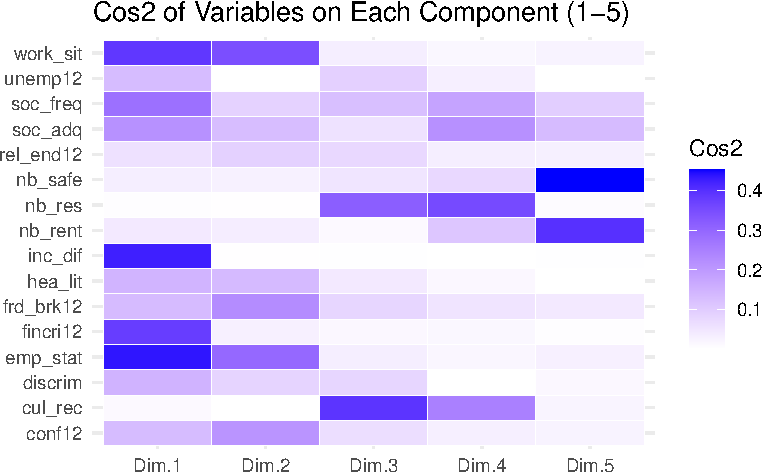
\includegraphics[width=0.7\textwidth,height=\textheight]{draft_v1_files/figure-pdf/unnamed-chunk-14-1.pdf}
\end{center}

\begin{itemize}
\item
  \textbf{Dim.1}: Variables \texttt{emp\_stat}, \texttt{work\_sit},
  \texttt{inc\_dif}, and \texttt{fincri12} show high cos² values,
  meaning that PC1 primarily captures variations in employment and
  financial difficulties. This component could represent
  \emph{employment \& finance} precariousness.
\item
  \textbf{Dim.2}: Variables \texttt{work\_sit}, \texttt{emp\_stat},
  \texttt{frd\_brk12}, and \texttt{conf12} are well-represented in this
  component, suggesting PC2 captures aspects of \emph{recent
  relationship stressors}.
\item
  \textbf{Dim.3}: Variables \texttt{nb\_res} and \texttt{cul\_rec} load
  strongly on PC3. This may represent community or cultural resources,
  indicating that this component is associated with \emph{neighborhood
  resources}.
\item
  \textbf{Dim.4}: This component has high cos² values for
  \texttt{nb\_res}, \texttt{cul\_rec}, \texttt{soc\_freq}, and
  \texttt{soc\_adq.} While \texttt{nb\_res} and \texttt{cul\_rec} are
  also prominent in PC3, PC4 uniquely captures nuanced differentiation
  in \emph{social} precariousness.
\item
  \textbf{Dim.5}: \texttt{nb\_safe} and \texttt{nb\_rent} are
  well-represented by PC5. This component might capture \emph{housing}
  precariousness.
\end{itemize}

\subsection{ICA}\label{ica}

\begin{center}
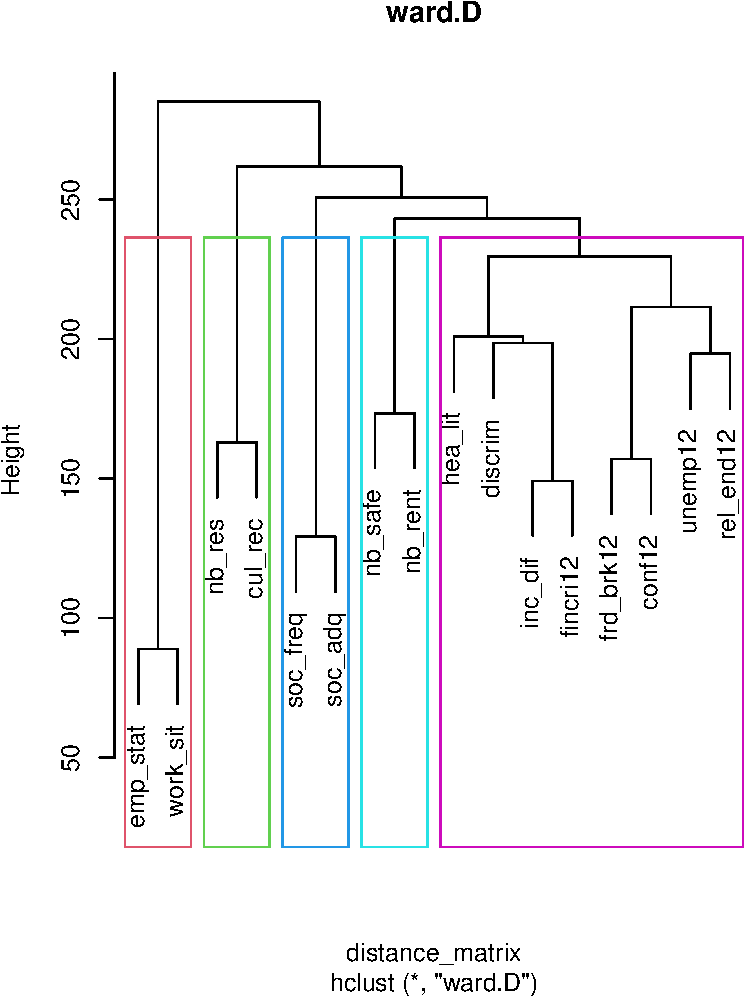
\includegraphics[width=0.7\textwidth,height=\textheight]{draft_v1_files/figure-pdf/unnamed-chunk-15-1.pdf}
\end{center}

\subsubsection{Dominant Variables per
Component:}\label{dominant-variables-per-component}

For each Independent Component (IC), we can identify variables with
\emph{high absolute} values in each column. These values indicate that
the IC captures a strong, independent signal associated with these
variables.

\begin{itemize}
\item
  \textbf{IC1}: \texttt{soc\_freq} and \texttt{soc\_adq} have strong
  negative loadings on this component, indicating that this component
  might represent \emph{social} precariousness.
\item
  \textbf{IC2}: \texttt{frd\_brk12}, \texttt{conf12},
  \texttt{rel\_end12}, \texttt{fincri12} and \texttt{unemp12} have the
  most substantial loadings on this component, all with negative signs.
  This might point to a \emph{recent relational or social stressor}
  component.
\item
  \textbf{IC3}: \texttt{nb\_res} and \texttt{cul\_rec} show notable
  negative loadings, pointing to a focus on \emph{community resource}
  precariousness.
\item
  \textbf{IC4}: High loadings for \texttt{nb\_safe}, \texttt{nb\_rent},
  \texttt{nb\_res}, \texttt{cul\_rec}, and \texttt{discrim} suggest a
  theme of \emph{housing and community-based} precariousness, reflecting
  both safety and social challenges within the neighborhood context.
\item
  \textbf{IC5}: \texttt{emp\_stat} and \texttt{work\_sit} both have
  strong negative loadings on this component, suggesting it captures
  \emph{employment} precariousness.
\end{itemize}

\subsection{Hierarchical clustering}\label{hierarchical-clustering}

\subsubsection{Using Euclidean distance}\label{using-euclidean-distance}

\begin{itemize}
\tightlist
\item
  Ward.D's method: Minimizes the variance within clusters, producing
  more compact and spherical clusters.
\item
  Single linkage: Groups clusters based on the minimum distance between
  points.
\item
  Complete linkage: Groups clusters based on the maximum distance
  between points.
\item
  Average linkage: Uses the average distance between all pairs of points
  in the two clusters.
\end{itemize}

\begin{figure}

\begin{minipage}{0.50\linewidth}
\begin{center}
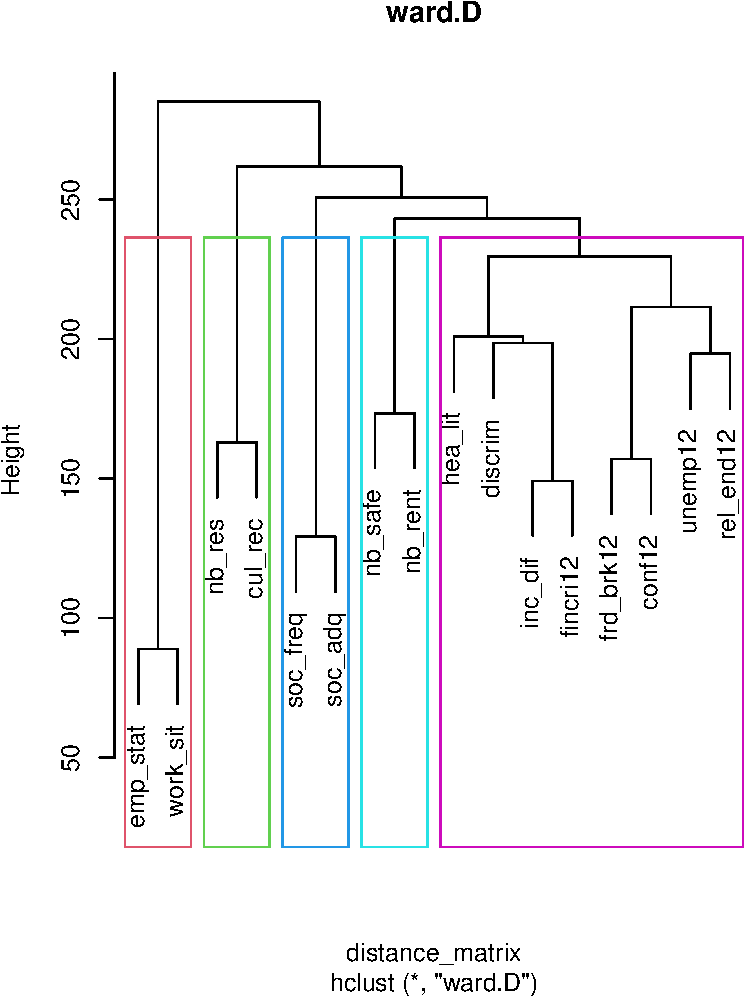
\includegraphics{draft_v1_files/figure-pdf/unnamed-chunk-16-1.pdf}
\end{center}
\end{minipage}%
%
\begin{minipage}{0.50\linewidth}
\begin{center}
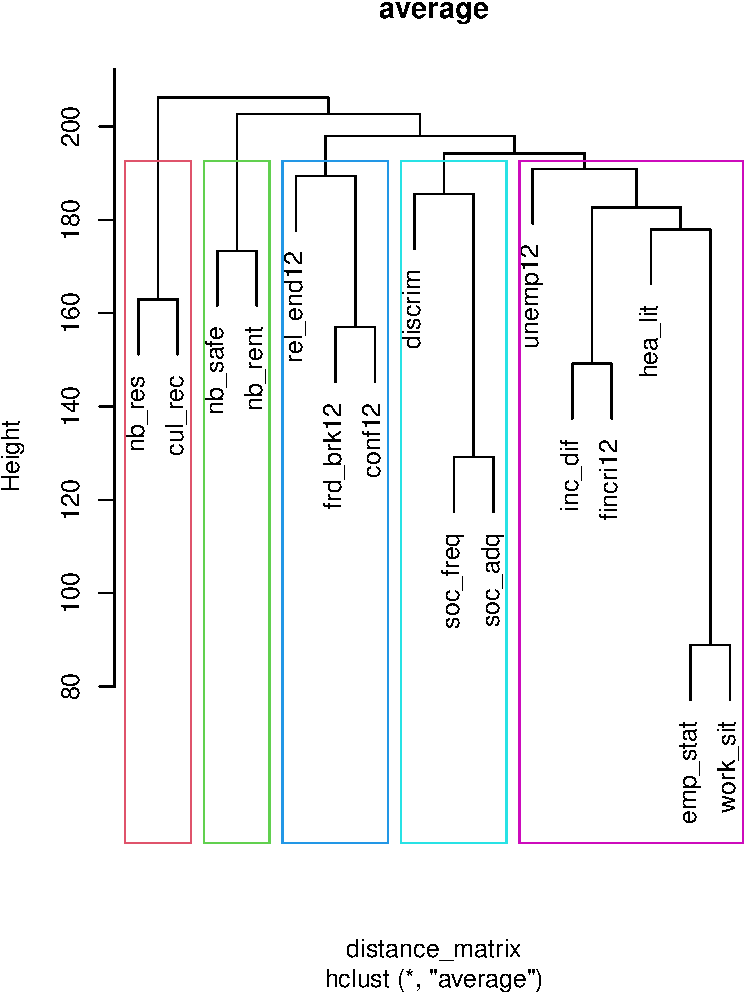
\includegraphics{draft_v1_files/figure-pdf/unnamed-chunk-16-2.pdf}
\end{center}
\end{minipage}%
\newline
\begin{minipage}{0.50\linewidth}
\begin{center}
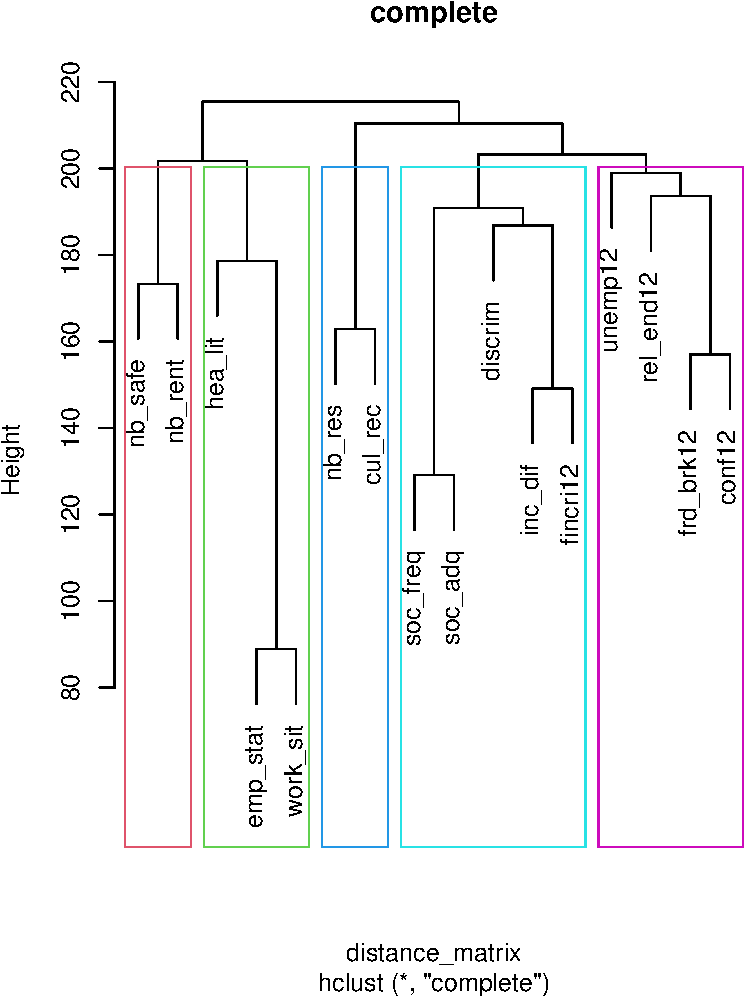
\includegraphics{draft_v1_files/figure-pdf/unnamed-chunk-16-3.pdf}
\end{center}
\end{minipage}%
%
\begin{minipage}{0.50\linewidth}
\begin{center}
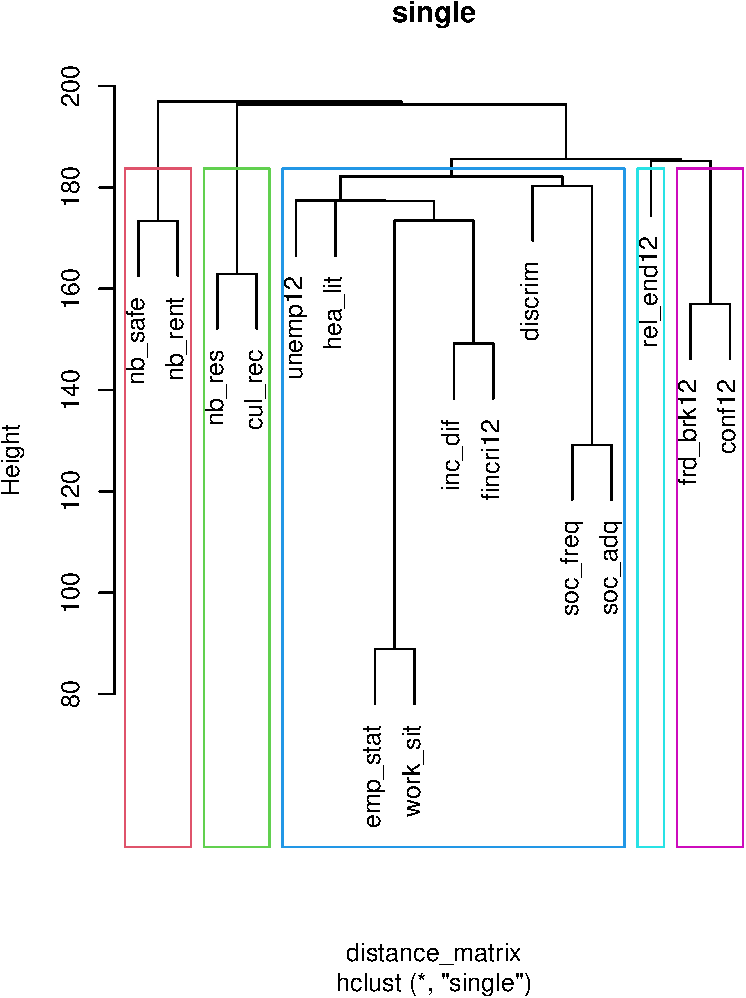
\includegraphics{draft_v1_files/figure-pdf/unnamed-chunk-16-4.pdf}
\end{center}
\end{minipage}%

\end{figure}%

\paragraph{Consistent Groupings (Across All or Most
Methods)}\label{consistent-groupings-across-all-or-most-methods}

\begin{itemize}
\item
  \texttt{emp\_stat} and \texttt{work\_sit}: This pair consistently
  clusters together across all linkage methods, suggesting that they are
  closely related variables, likely capturing a similar aspect of the
  data (possibly employment status or employment-related information).
\item
  \texttt{nb\_safe}, \texttt{nb\_res}, and \texttt{nb\_rent}: These
  variables are often grouped closely in several methods (especially
  Ward.D, average, and complete linkage). This suggests a similarity or
  common theme among them, potentially related to neighborhood or
  housing precariousness.
\item
  \texttt{soc\_freq} and \texttt{soc\_adq}: These two variables
  frequently cluster together, indicating they likely measure aspects of
  social frequency and adequacy in similar ways. They appear together in
  Ward.D, average, and complete linkage.
\item
  \texttt{frd\_brk12} and \texttt{conf12}: These variables are often
  clustered closely (though they sometimes join with other variables
  like rel\_end12), suggesting they may capture aspects of relationship
  or social conflict. This pair appears in close proximity, especially
  in average and Ward.D.
\end{itemize}

\paragraph{Inconsistent Groupings (Variability Across
Methods)}\label{inconsistent-groupings-variability-across-methods}

\begin{itemize}
\item
  \texttt{hea\_lit}: This variable shows inconsistent clustering across
  methods. In Ward.D, it joins with \texttt{fincri12}, while in other
  methods, it's often more isolated or grouped with variables that do
  not appear similar. This may suggest that \texttt{hea\_lit} does not
  strongly correlate with other variables, or it has multidimensional
  aspects affecting its grouping across methods.
\item
  \texttt{discrim}: This variable also shows variable groupings. In
  Ward.D, it is grouped with \texttt{hea\_lit}, while in other methods
  (e.g., complete and single linkage), it clusters differently,
  sometimes on its own. This variability may indicate that
  \texttt{discrim} has weaker associations with the main clusters in the
  data or overlaps partially with multiple clusters.
\item
  Social and Financial Variables (\texttt{inc\_dif}, \texttt{fincri12},
  \texttt{unemp12}): These variables appear together in some methods
  (e.g., Ward.D clusters \texttt{fincri12} and \texttt{inc\_dif}), but
  in others, they are spread out. This inconsistency suggests that
  social and financial variables may not have strong or consistent ties
  across different methods, perhaps due to capturing different aspects
  of precariousness.
\end{itemize}

\paragraph{Summary}\label{summary-1}

The consistent clusters are likely capturing distinct thematic
dimensions of the data (e.g., employment, housing, social contact),
while the inconsistent variables may reflect multifaceted or weakly
correlated attributes that do not fit neatly into one cluster.

\subsubsection{Using Mutual Information}\label{using-mutual-information}

Using mutual information (MI) as a basis for hierarchical clustering
differs from using traditional distance measures (like Euclidean
distance) in a few key ways.

\begin{center}
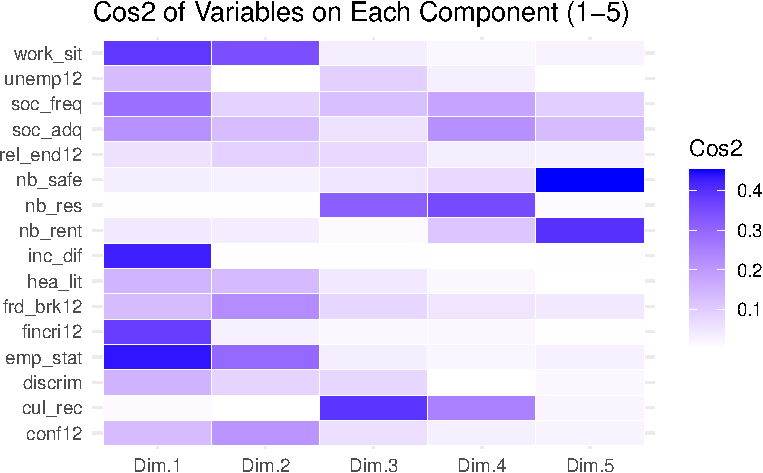
\includegraphics[width=0.6\textwidth,height=\textheight]{draft_v1_files/figure-pdf/unnamed-chunk-17-1.pdf}
\end{center}

\paragraph{Comparison to Euclidean Distance
Clustering}\label{comparison-to-euclidean-distance-clustering}

\begin{itemize}
\item
  \textbf{Housing and Community} Cluster: The variables
  \texttt{nb\_safe}, \texttt{nb\_res}, \texttt{nb\_rent}, and
  \texttt{cul\_rec} cluster together, indicating a strong association
  among housing-related and community-based factors. This suggests a
  shared theme of housing or community precariousness. This grouping is
  also observed in the Euclidean-based clustering, but it appears more
  tightly connected here, potentially due to the non-linear
  relationships highlighted by mutual information.
\item
  \textbf{Employment and Social Support} Cluster: \texttt{emp\_stat} and
  \texttt{work\_sit} form a cluster, linking employment status and work
  situation together as they did in Euclidean-based clustering. These
  remain closely associated regardless of the distance metric used.
  \texttt{soc\_freq} and \texttt{soc\_adq}, related to social contact
  frequency and adequacy, cluster nearby, indicating they have a
  stronger non-linear relationship with employment variables. This is a
  subtle difference as Euclidean distance might not capture this
  association as effectively.
\item
  \textbf{Financial Stressor} Cluster: \texttt{inc\_dif} and
  \texttt{fincri12}, representing income difficulties and recent
  financial crises, consistently cluster together in both approaches,
  showing a strong association, likely linear. However, mutual
  information-based clustering links these financial stressors with
  social support variables, suggesting that financial challenges may
  have complex dependencies with social support in this dataset.
\item
  \textbf{Relational Stressor} Cluster: \texttt{frd\_brk12},
  \texttt{conf12}, \texttt{discrim}, \texttt{hea\_lit},
  \texttt{unemp12}, and \texttt{rel\_end12} form a \emph{looser} cluster
  focused on social and relational stressors (e.g., friendship breakup,
  conflicts, and discrimination). Compared to Euclidean clustering,
  \texttt{discrim} and \texttt{hea\_lit} (health literacy) appear closer
  to relational stressors here, indicating that non-linear relationships
  might play a larger role in linking these variables.
\end{itemize}

\paragraph{Summary}\label{summary-2}

In conclusion, mutual information-based clustering provides an
alternative perspective that can reveal more intricate associations
between variables, especially for those with non-linear relationships.
Compared to Euclidean clustering, it shows a similar high-level
structure but emphasizes nuanced connections between variables,
particularly around social support, employment, and financial stress.

\subsection{Conclusions on Precariousness
factors}\label{conclusions-on-precariousness-factors}

Based on the consistent findings across multiple analyses, we decided to
exclude the variables \texttt{discrim}, \texttt{hea\_lit},
\texttt{umemp12}, and \texttt{rel\_end12}, as they do not clearly belong
to any specific precariousness factor nor exhibit strong associations
with depression (see the correlation table above). Therefore, we propose
retaining the following key precariousness factors:

\begin{itemize}
\tightlist
\item
  Employment Precariousness: \texttt{emp\_stat}, \texttt{work\_sit}
\item
  Social Precariousness: \texttt{soc\_freq}, \texttt{soc\_adq}
\item
  Housing Precariousness: \texttt{nb\_safe}, \texttt{nb\_res},
  \texttt{nb\_rent}, \texttt{cul\_rec}
\item
  Recent Relational Stressors: \texttt{frd\_brk12}, \texttt{conf12}
\item
  Recent Financial Stressors: \texttt{fincri12}, \texttt{inc\_diff}
\end{itemize}

We construct each precariousness factor by calculating the mean value of
the combined variables. Below, we present the updated correlation table
for the newly composed factors, along with the corresponding
distributions of all variables to be used in the causal discovery
analysis.

\begin{center}
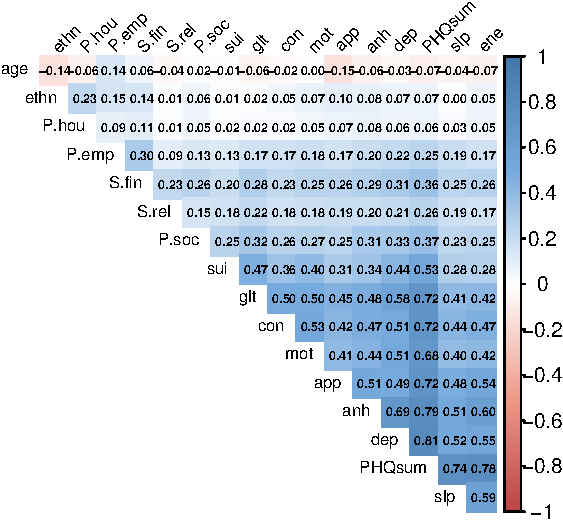
\includegraphics{draft_v1_files/figure-pdf/unnamed-chunk-18-1.pdf}
\end{center}

\begin{center}
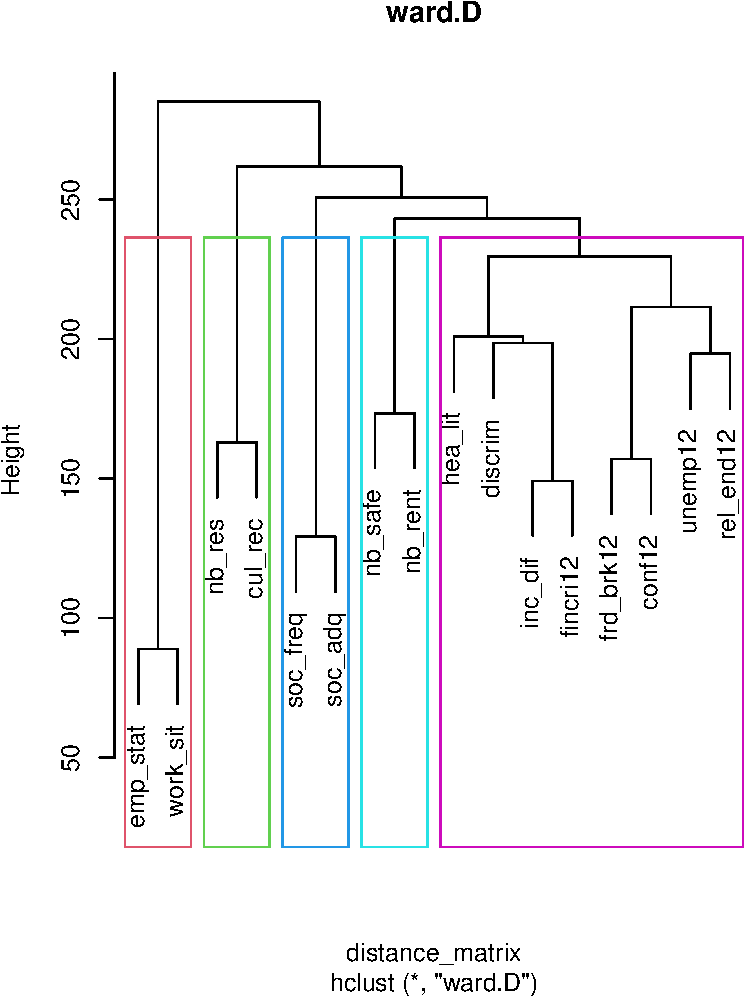
\includegraphics{draft_v1_files/figure-pdf/unnamed-chunk-19-1.pdf}
\end{center}

\subsection{Results from CCI
algorithm}\label{results-from-cci-algorithm}

\begin{figure}

\begin{minipage}{0.50\linewidth}

\centering{

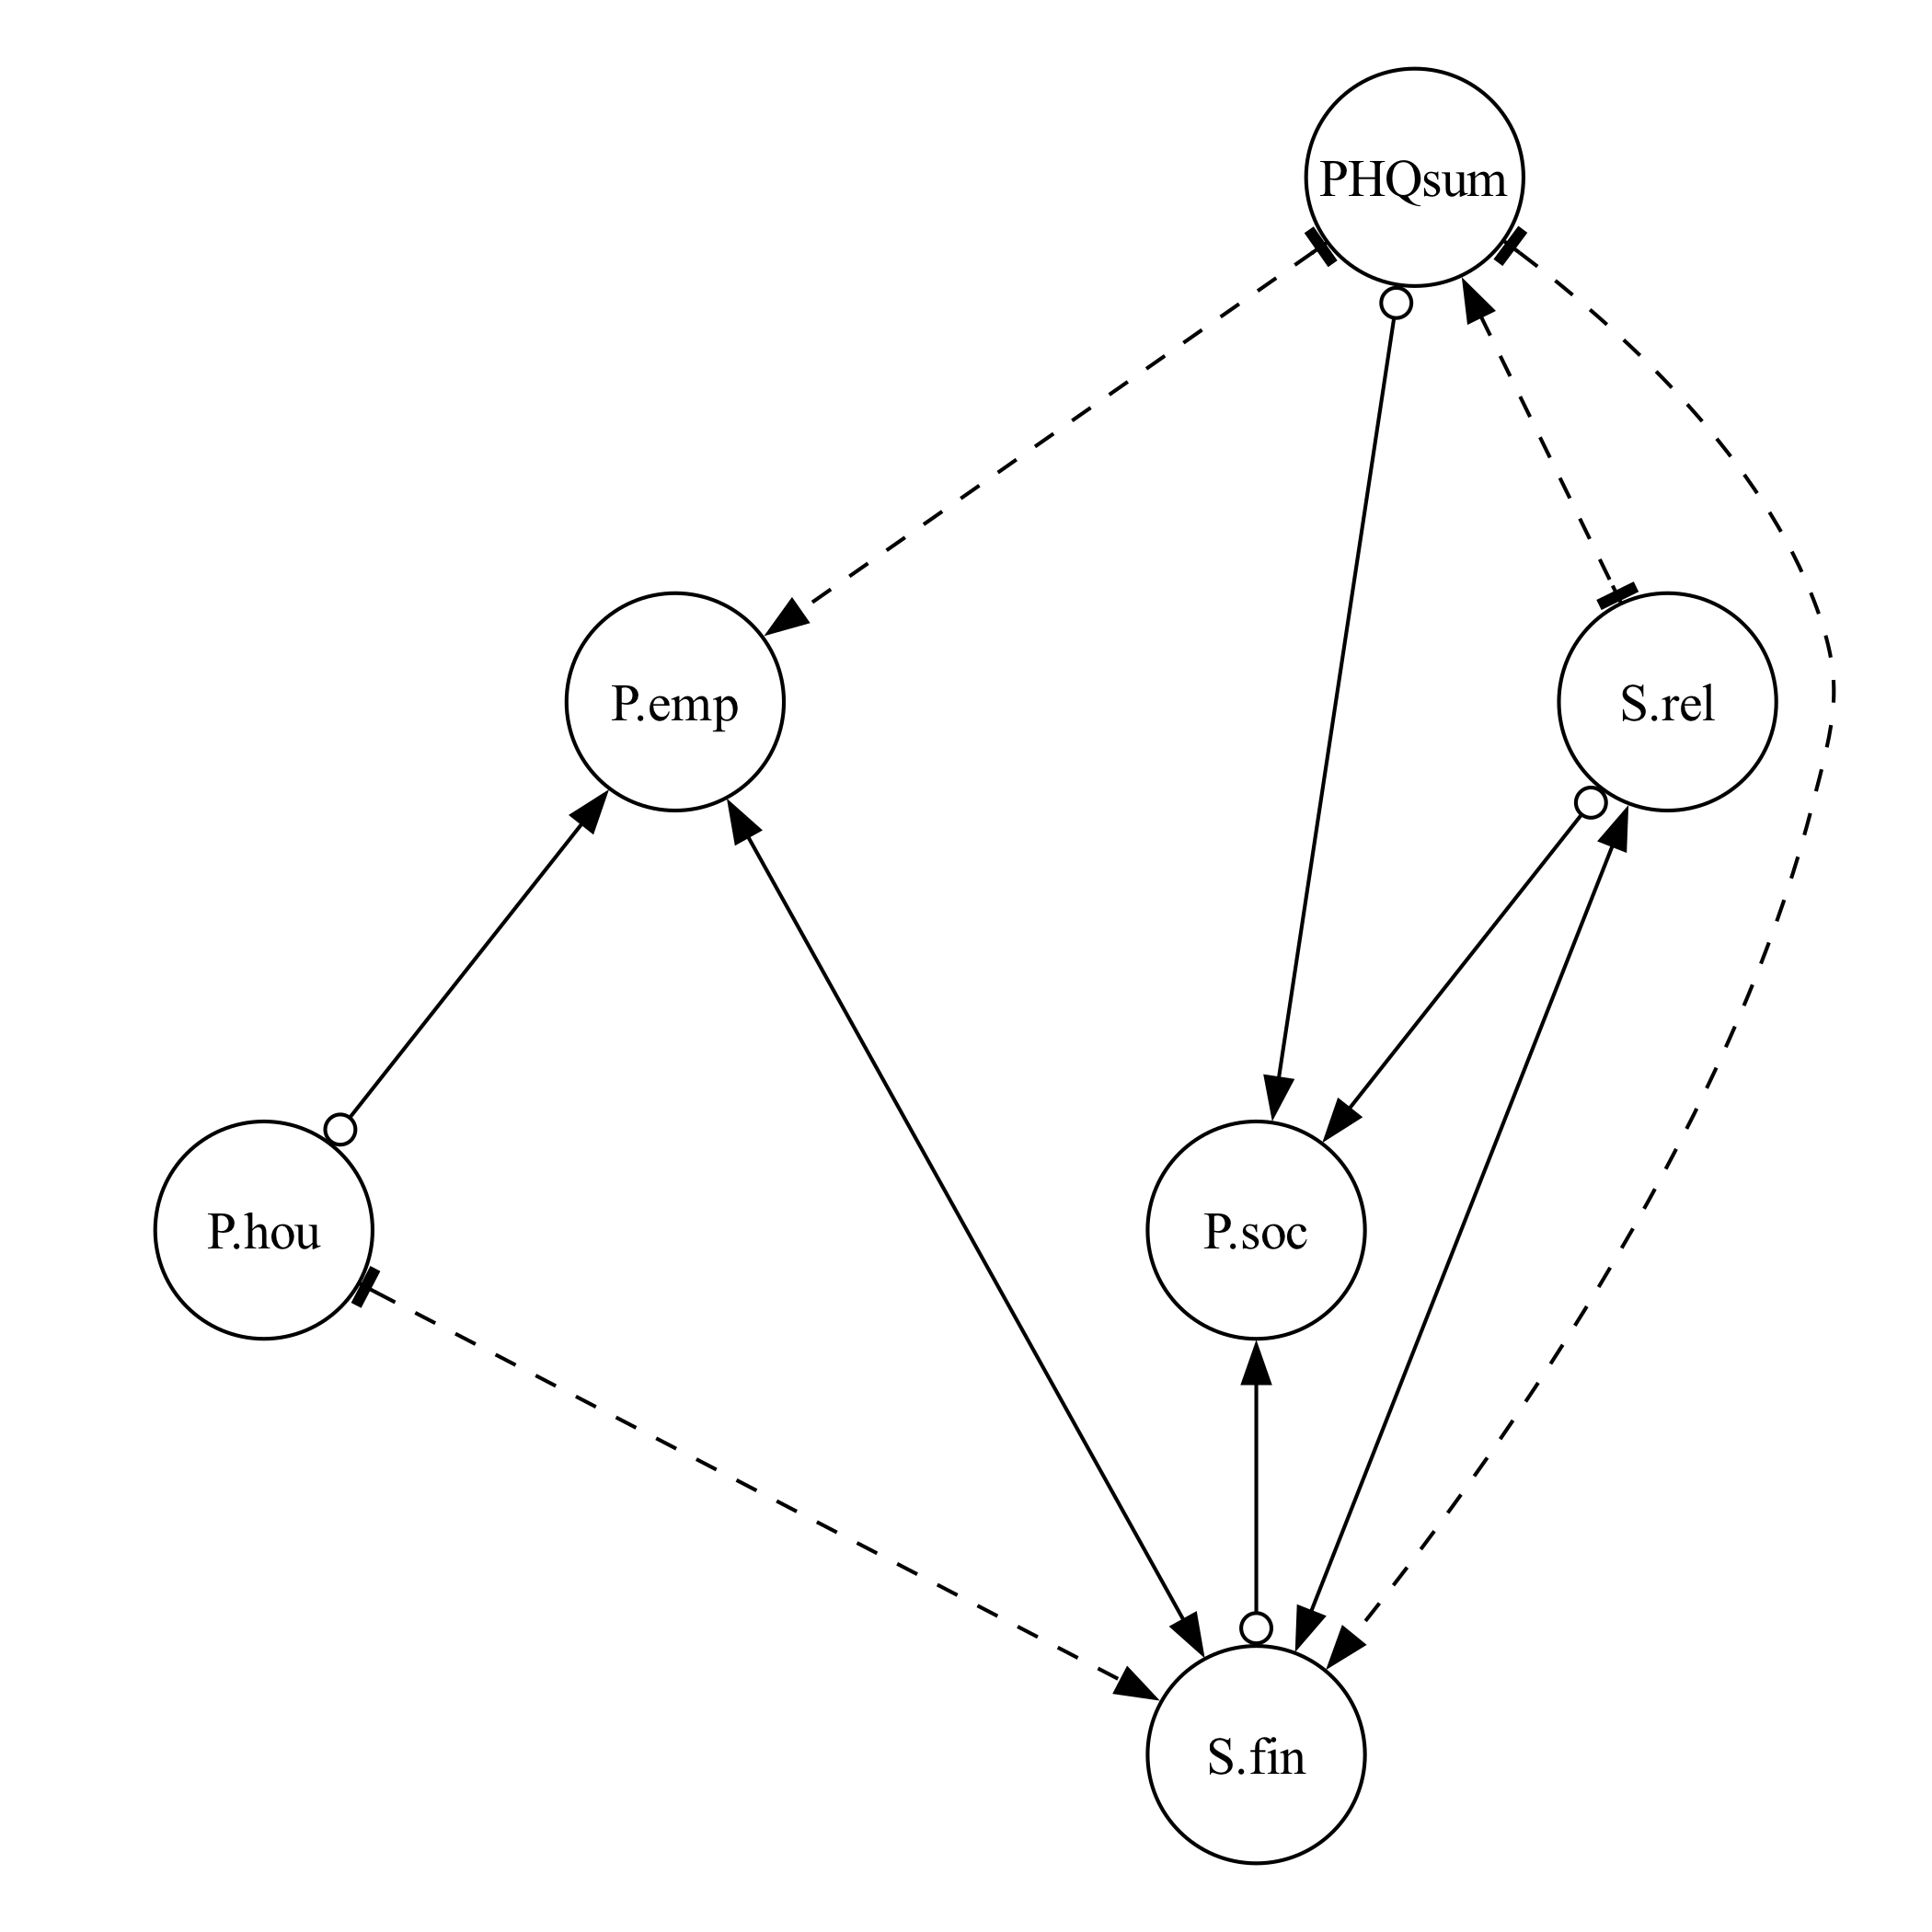
\includegraphics[width=1\textwidth,height=\textheight]{img/CCI_depsum.png}

}

\subcaption{\label{fig-sum-cci-1}CCI MAAG}

\end{minipage}%
%
\begin{minipage}{0.50\linewidth}

\centering{

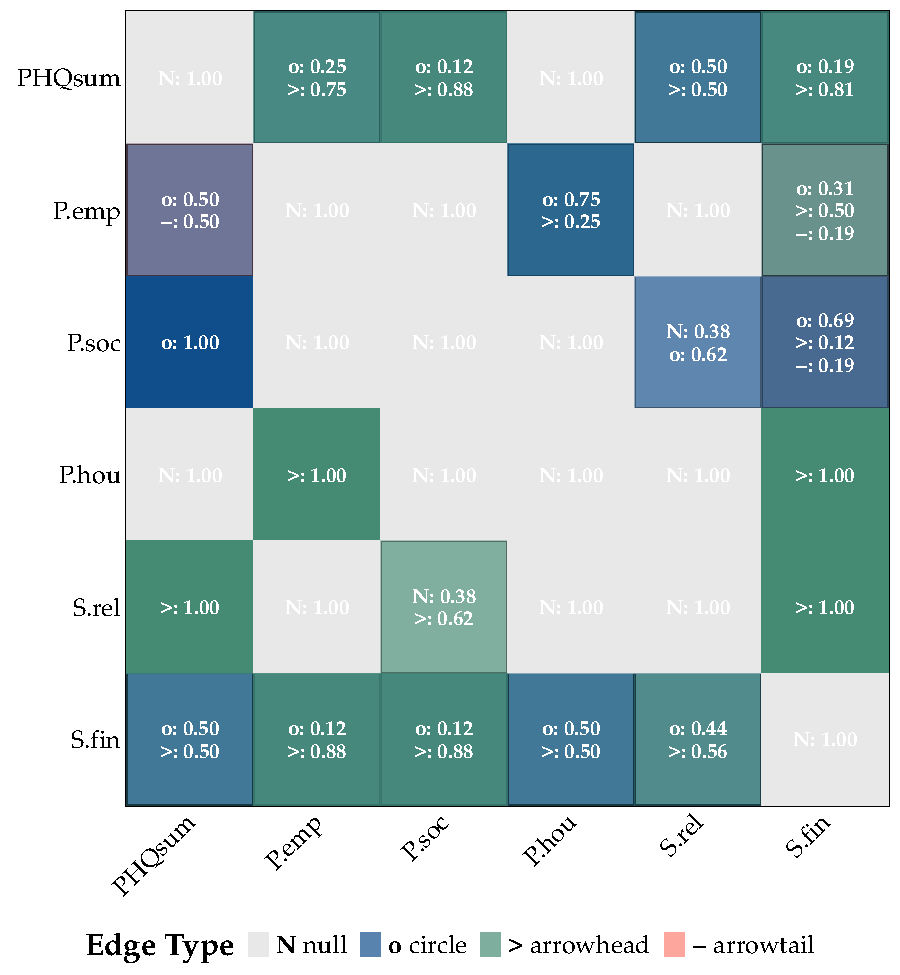
\includegraphics[width=1\textwidth,height=\textheight]{img/depsum_mat_cci.pdf}

}

\subcaption{\label{fig-sum-cci-2}Proportion matrix}

\end{minipage}%

\caption{\label{fig-sum-cci}Resulting graph of precarity factors and
depression sum score using CCI and proportion of edge endpoint types.}

\end{figure}%

\begin{figure}

\begin{minipage}{\linewidth}

\centering{

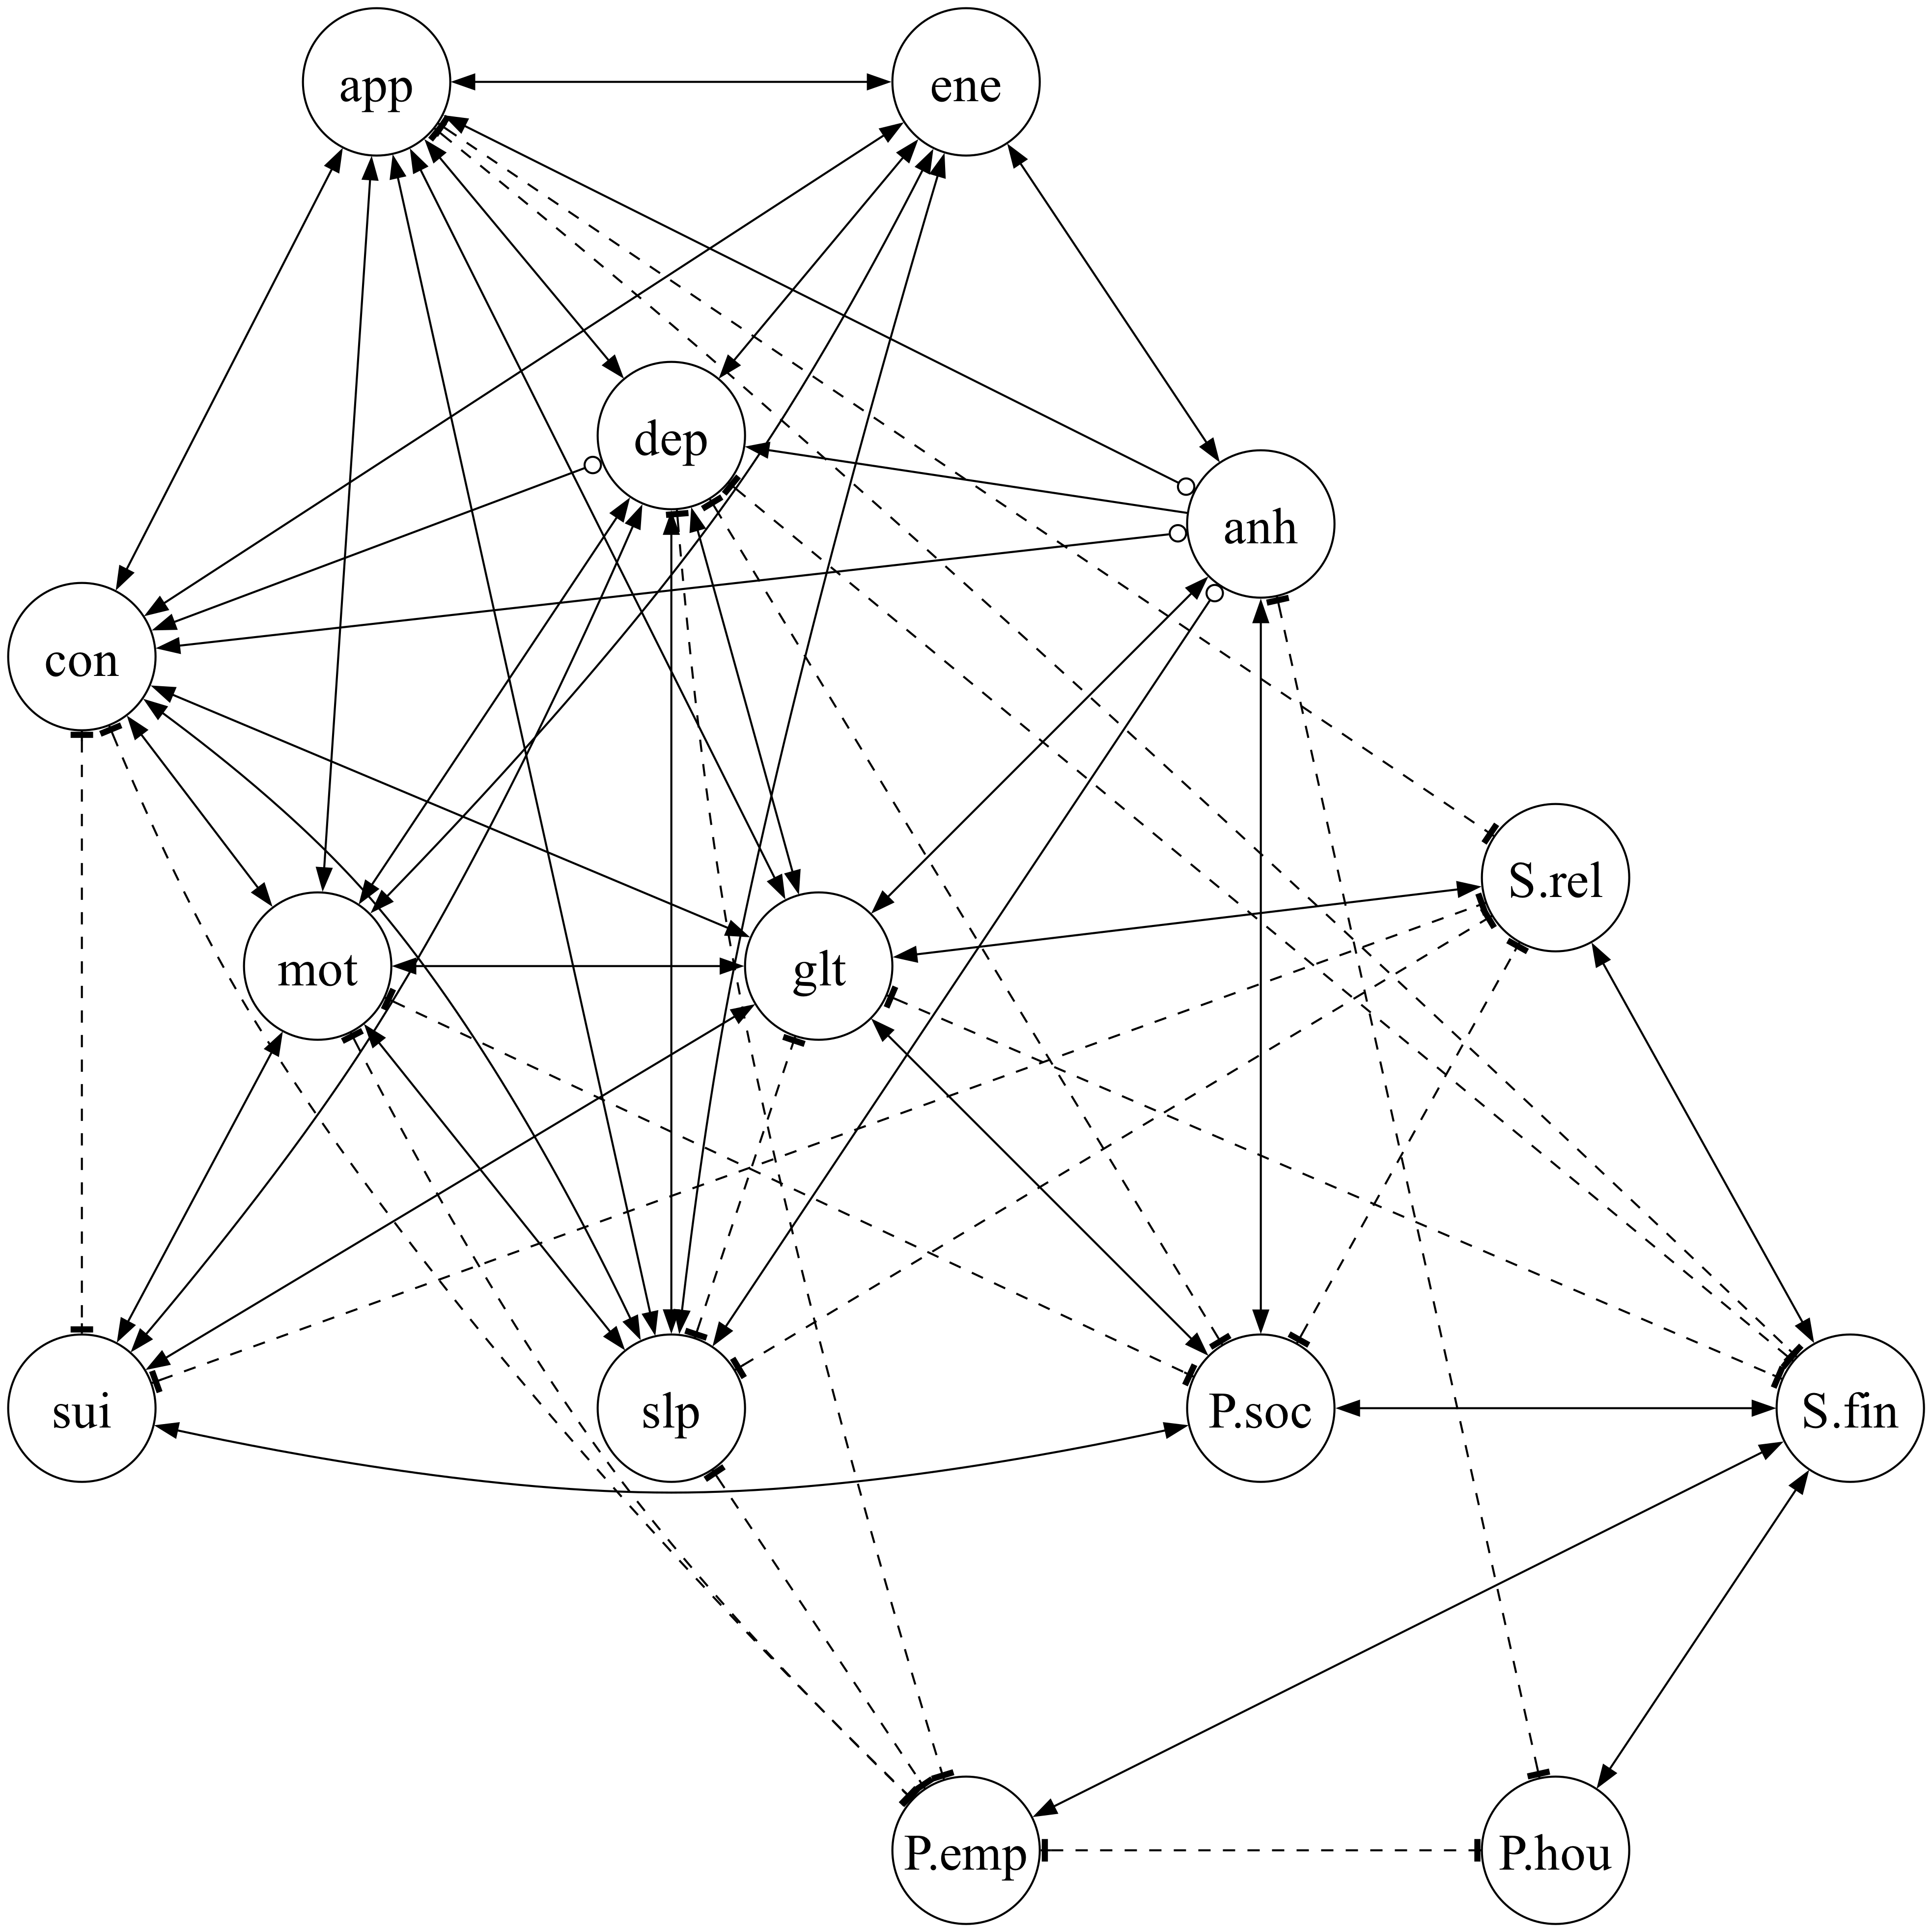
\includegraphics[width=0.6\textwidth,height=\textheight]{img/symptom_graph_CCI.png}

}

\subcaption{\label{fig-sym-cci-1}CCI MAAG}

\end{minipage}%
\newline
\begin{minipage}{\linewidth}

\centering{

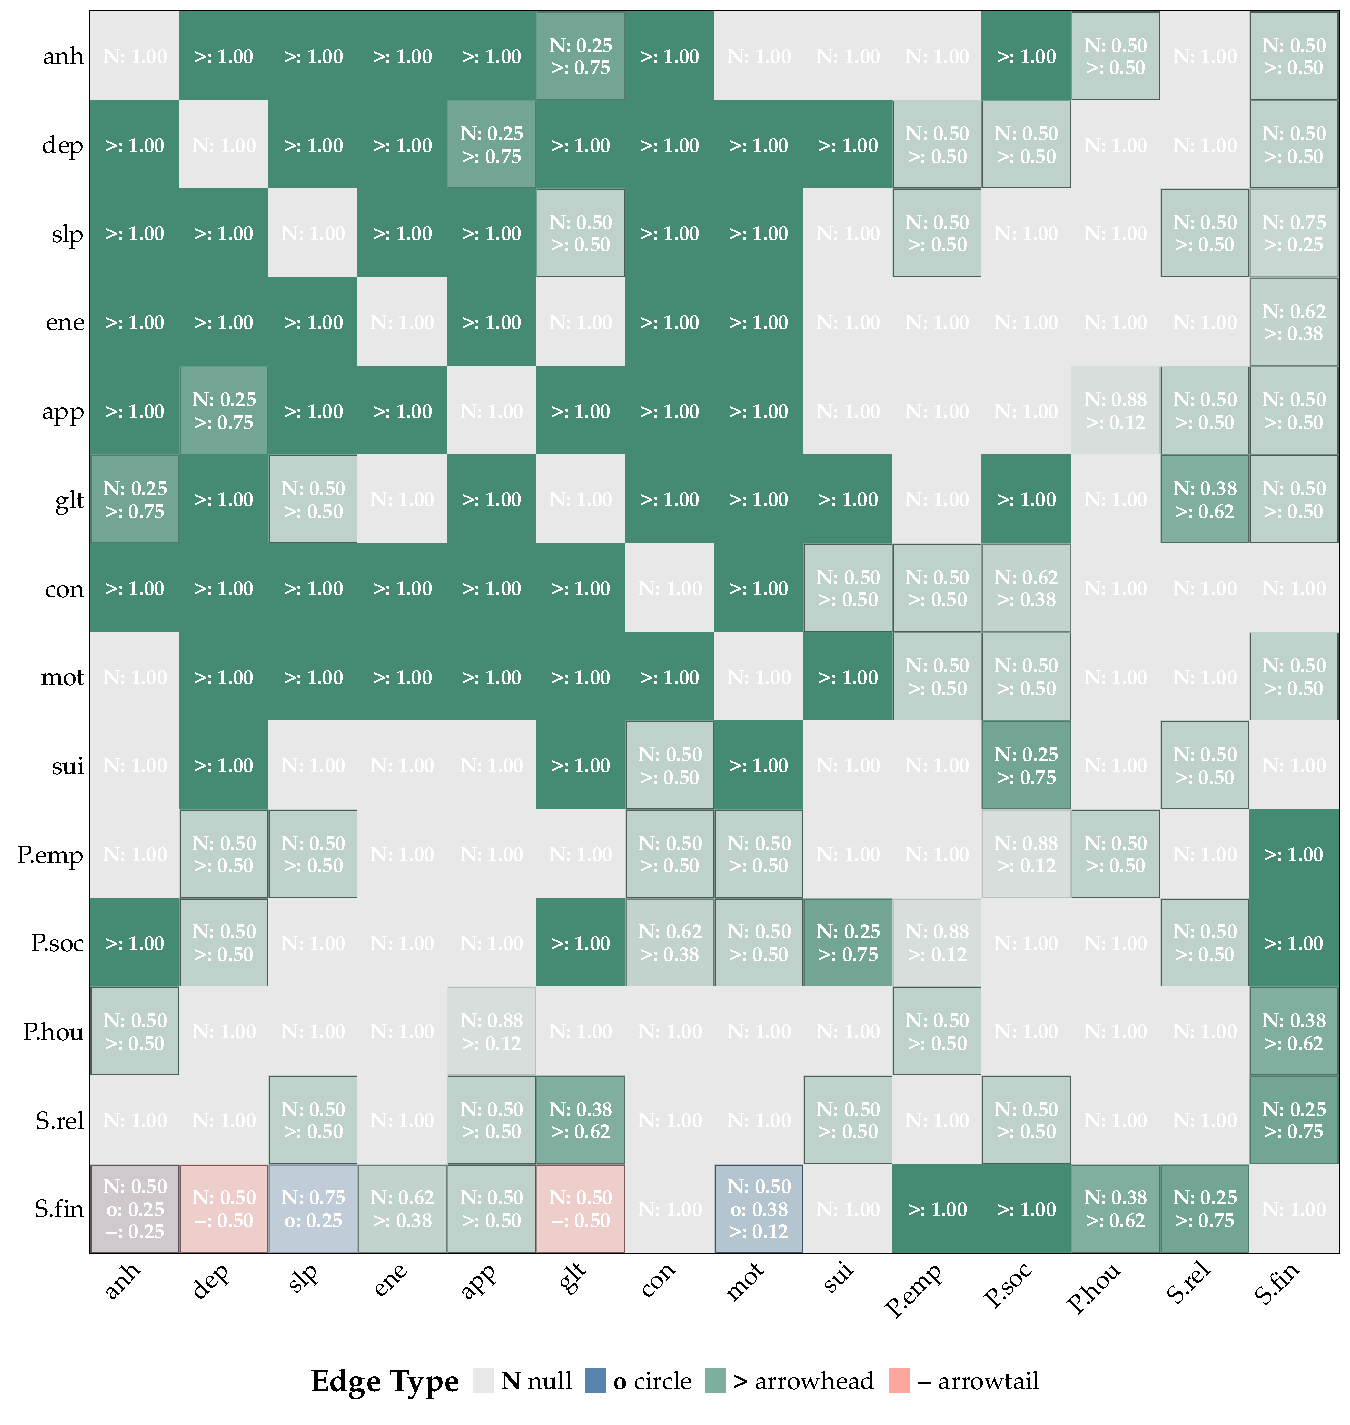
\includegraphics[width=0.6\textwidth,height=\textheight]{img/symptom_mat_cci.pdf}

}

\subcaption{\label{fig-sym-cci-2}Proportion matrix}

\end{minipage}%

\caption{\label{fig-sym-cci}Resulting graph of precarity factors and
individual depression symptoms using CCI and proportion of edge endpoint
types.}

\end{figure}%

\begin{figure}

\begin{minipage}{\linewidth}

\centering{

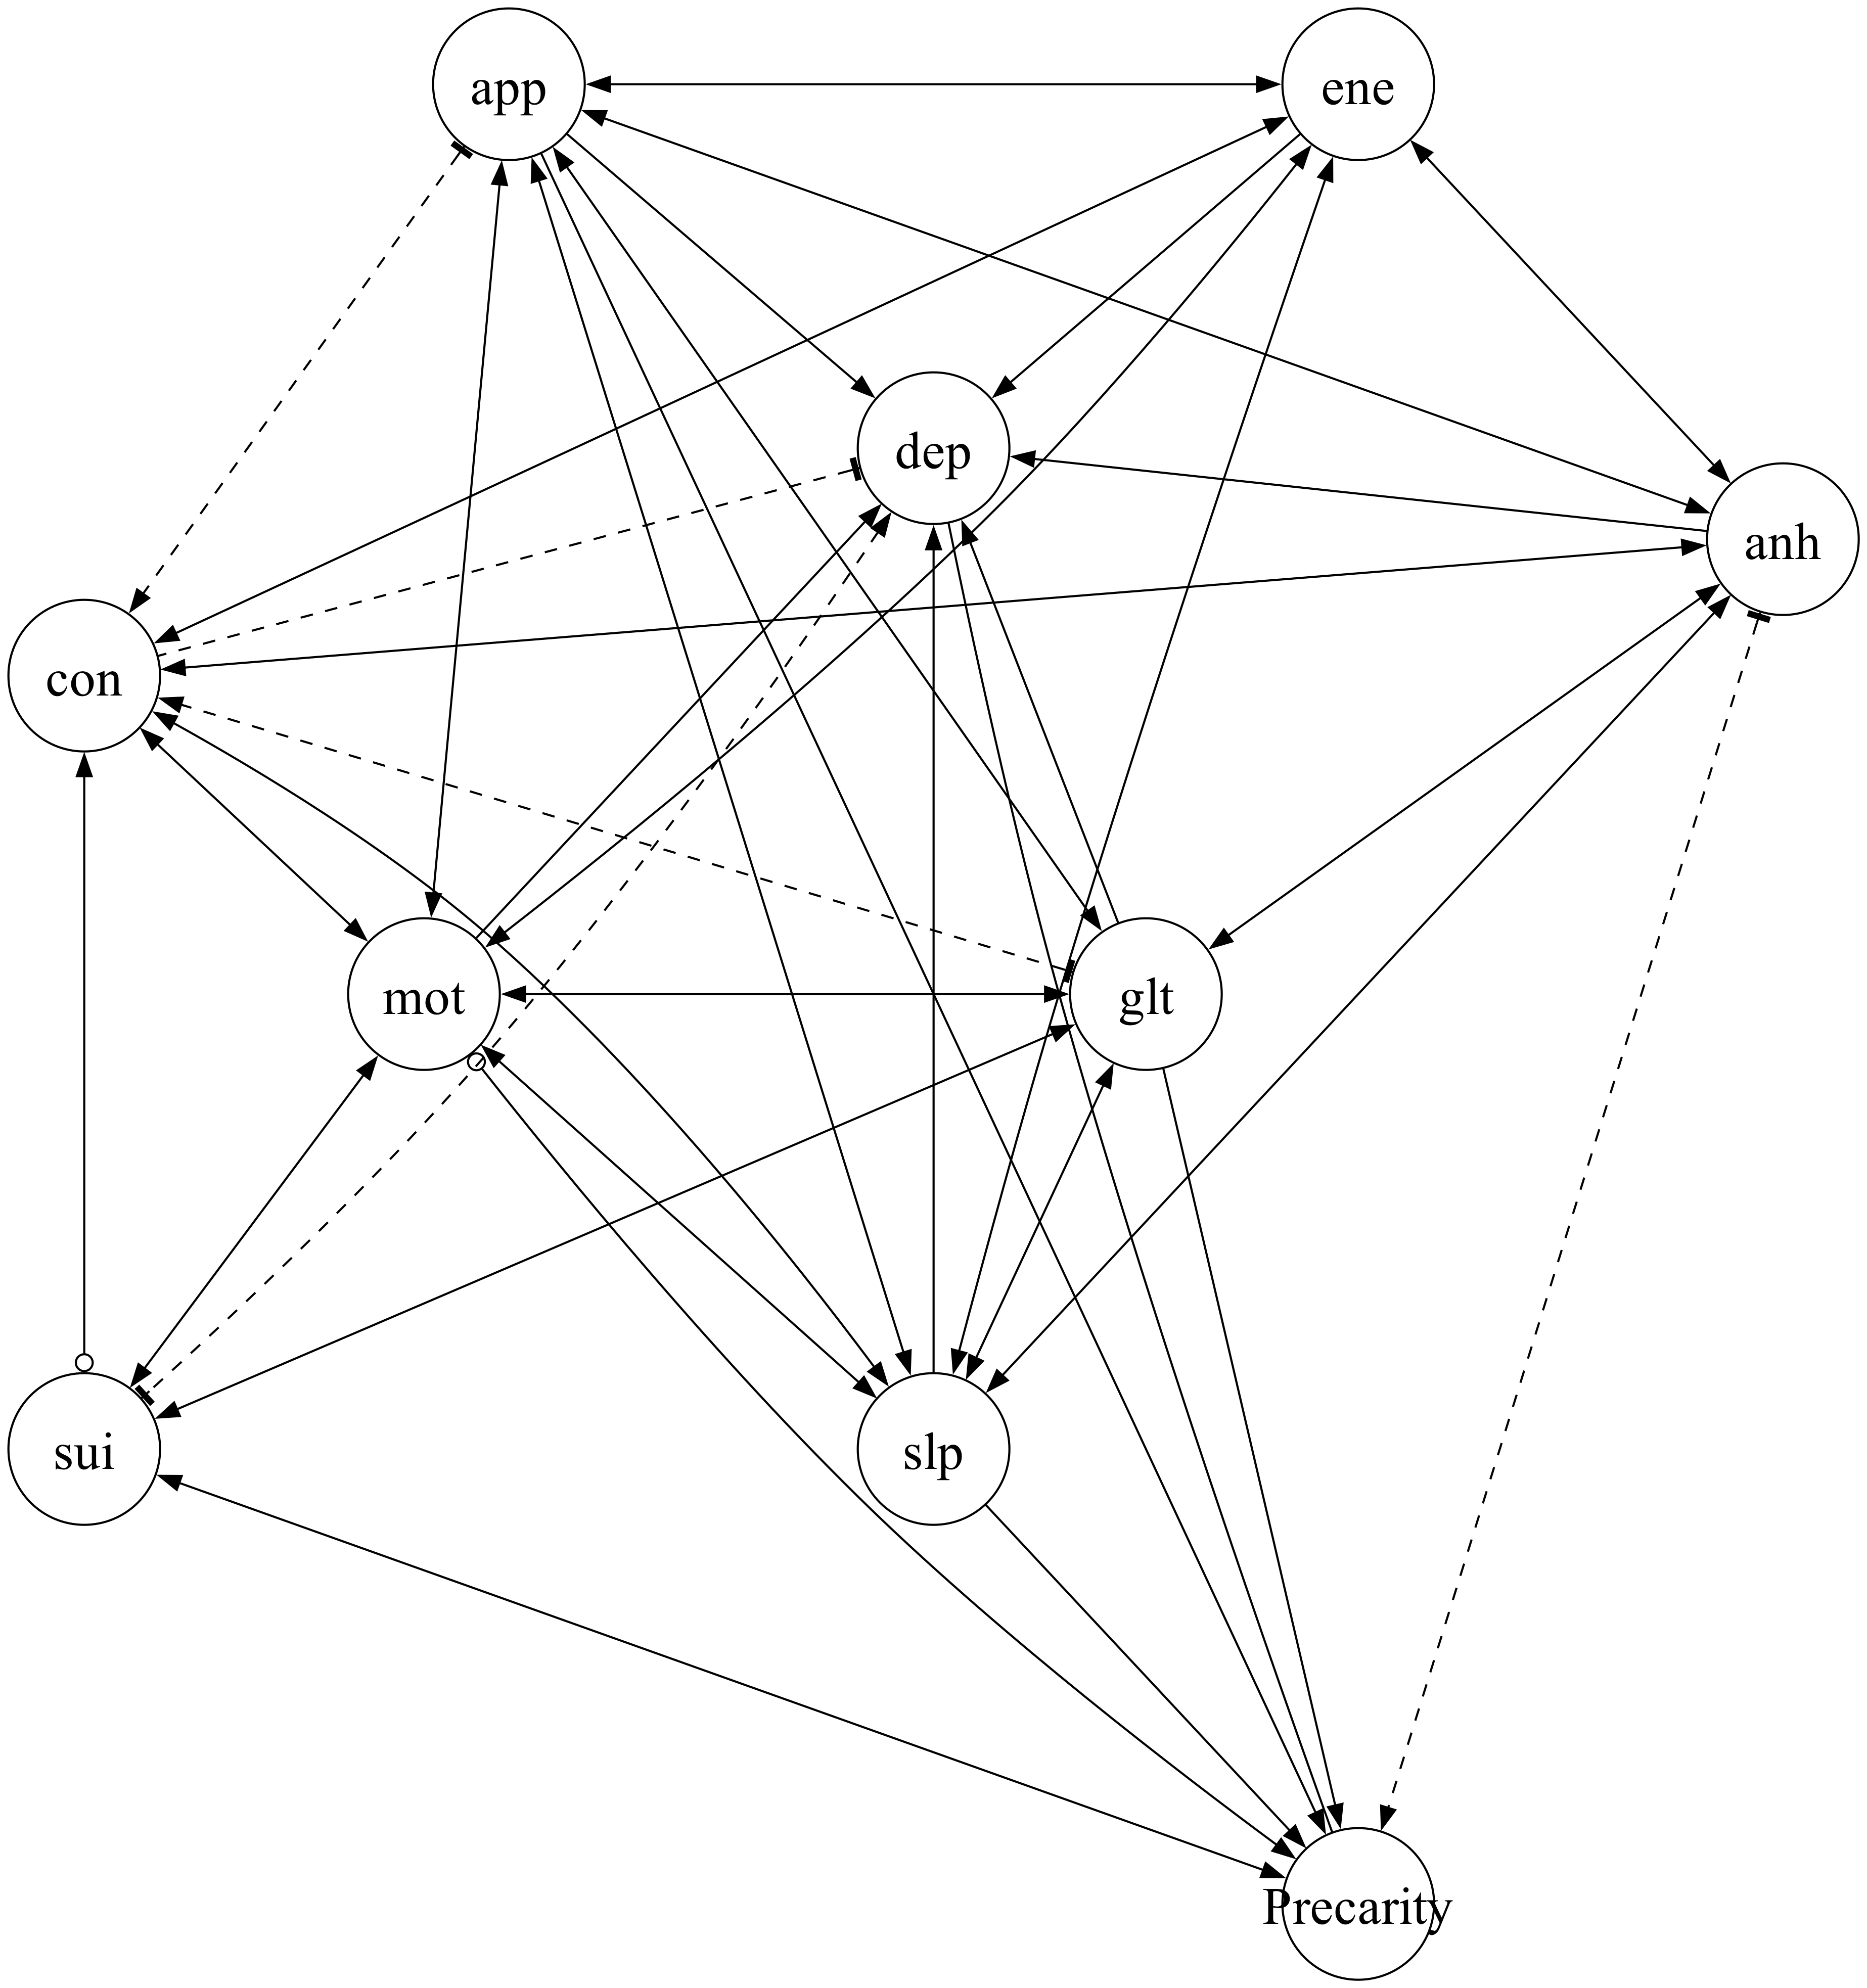
\includegraphics[width=0.6\textwidth,height=\textheight]{img/presum_graph_CCI.png}

}

\subcaption{\label{fig-presum-cci-1}CCI MAAG}

\end{minipage}%
\newline
\begin{minipage}{\linewidth}

\centering{

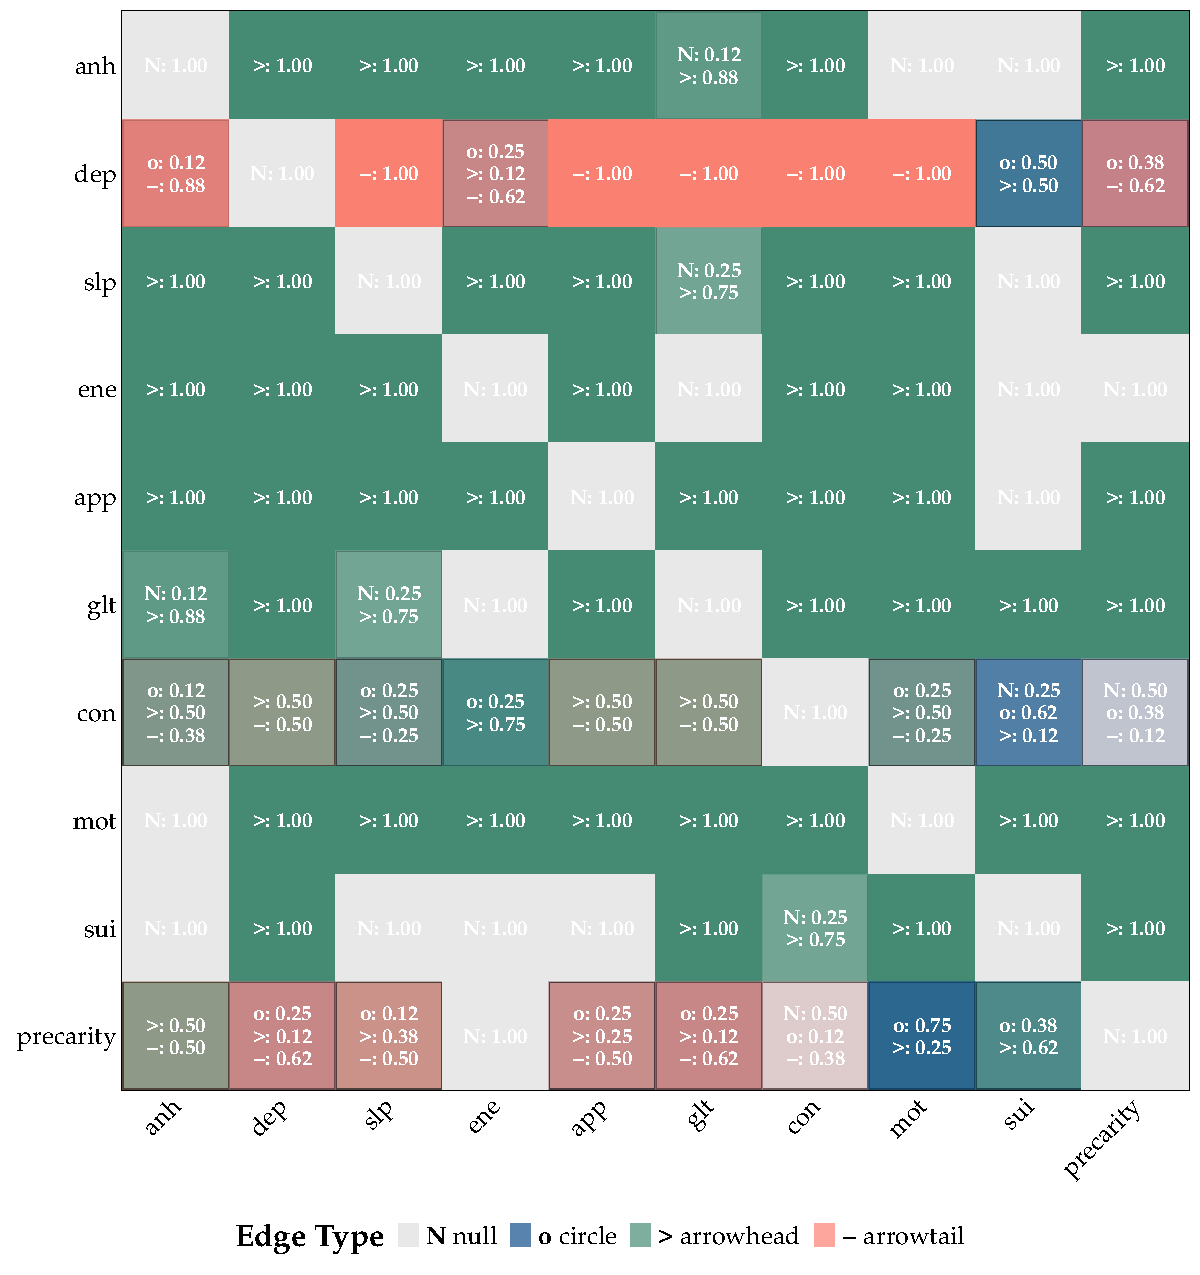
\includegraphics[width=0.6\textwidth,height=\textheight]{img/presum_mat_cci.pdf}

}

\subcaption{\label{fig-presum-cci-2}Proportion matrix}

\end{minipage}%

\caption{\label{fig-presum-cci}Resulting graph of precarity sum score
and individual depression symptoms using CCI and proportion of edge
endpoint types.}

\end{figure}%

\clearpage

\subsection{Results from PC algorithm}\label{results-from-pc-algorithm}

\begin{figure}

\begin{minipage}{0.50\linewidth}

\centering{

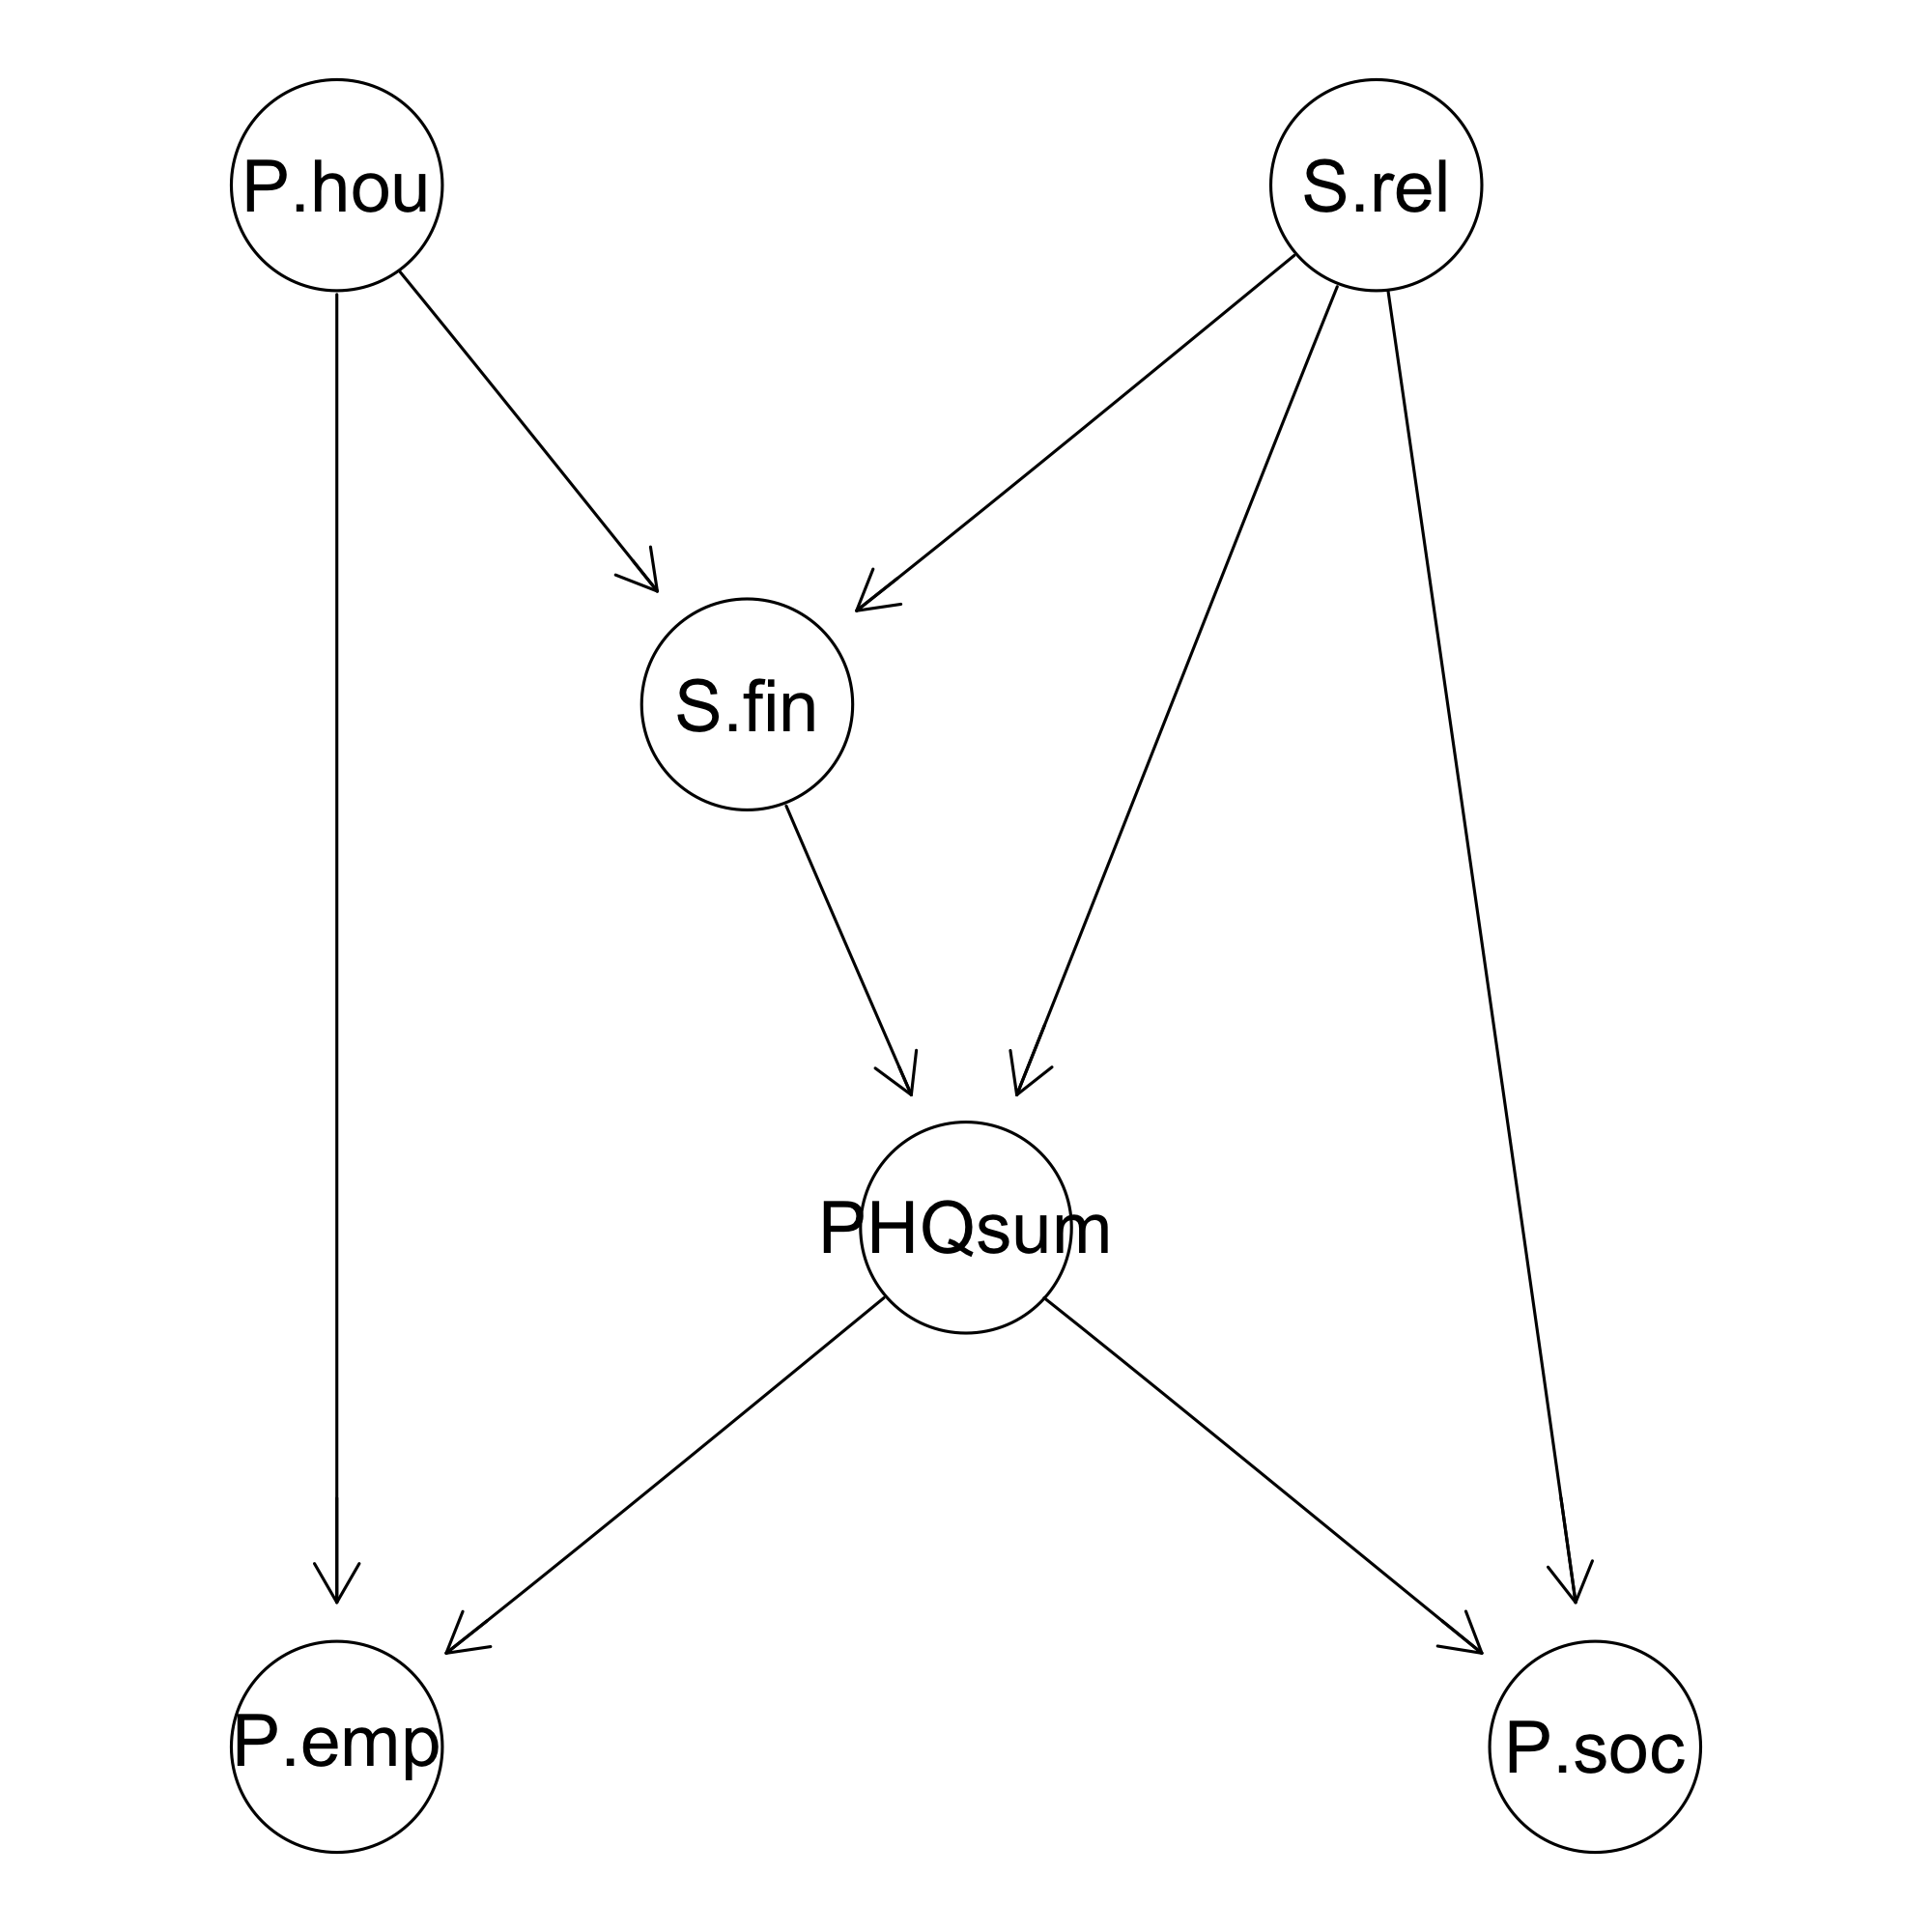
\includegraphics[width=1\textwidth,height=\textheight]{img/sum_PC_all.png}

}

\subcaption{\label{fig-pc_sum-1}Using both GaussianCI and RCoT}

\end{minipage}%
%
\begin{minipage}{0.50\linewidth}

\centering{

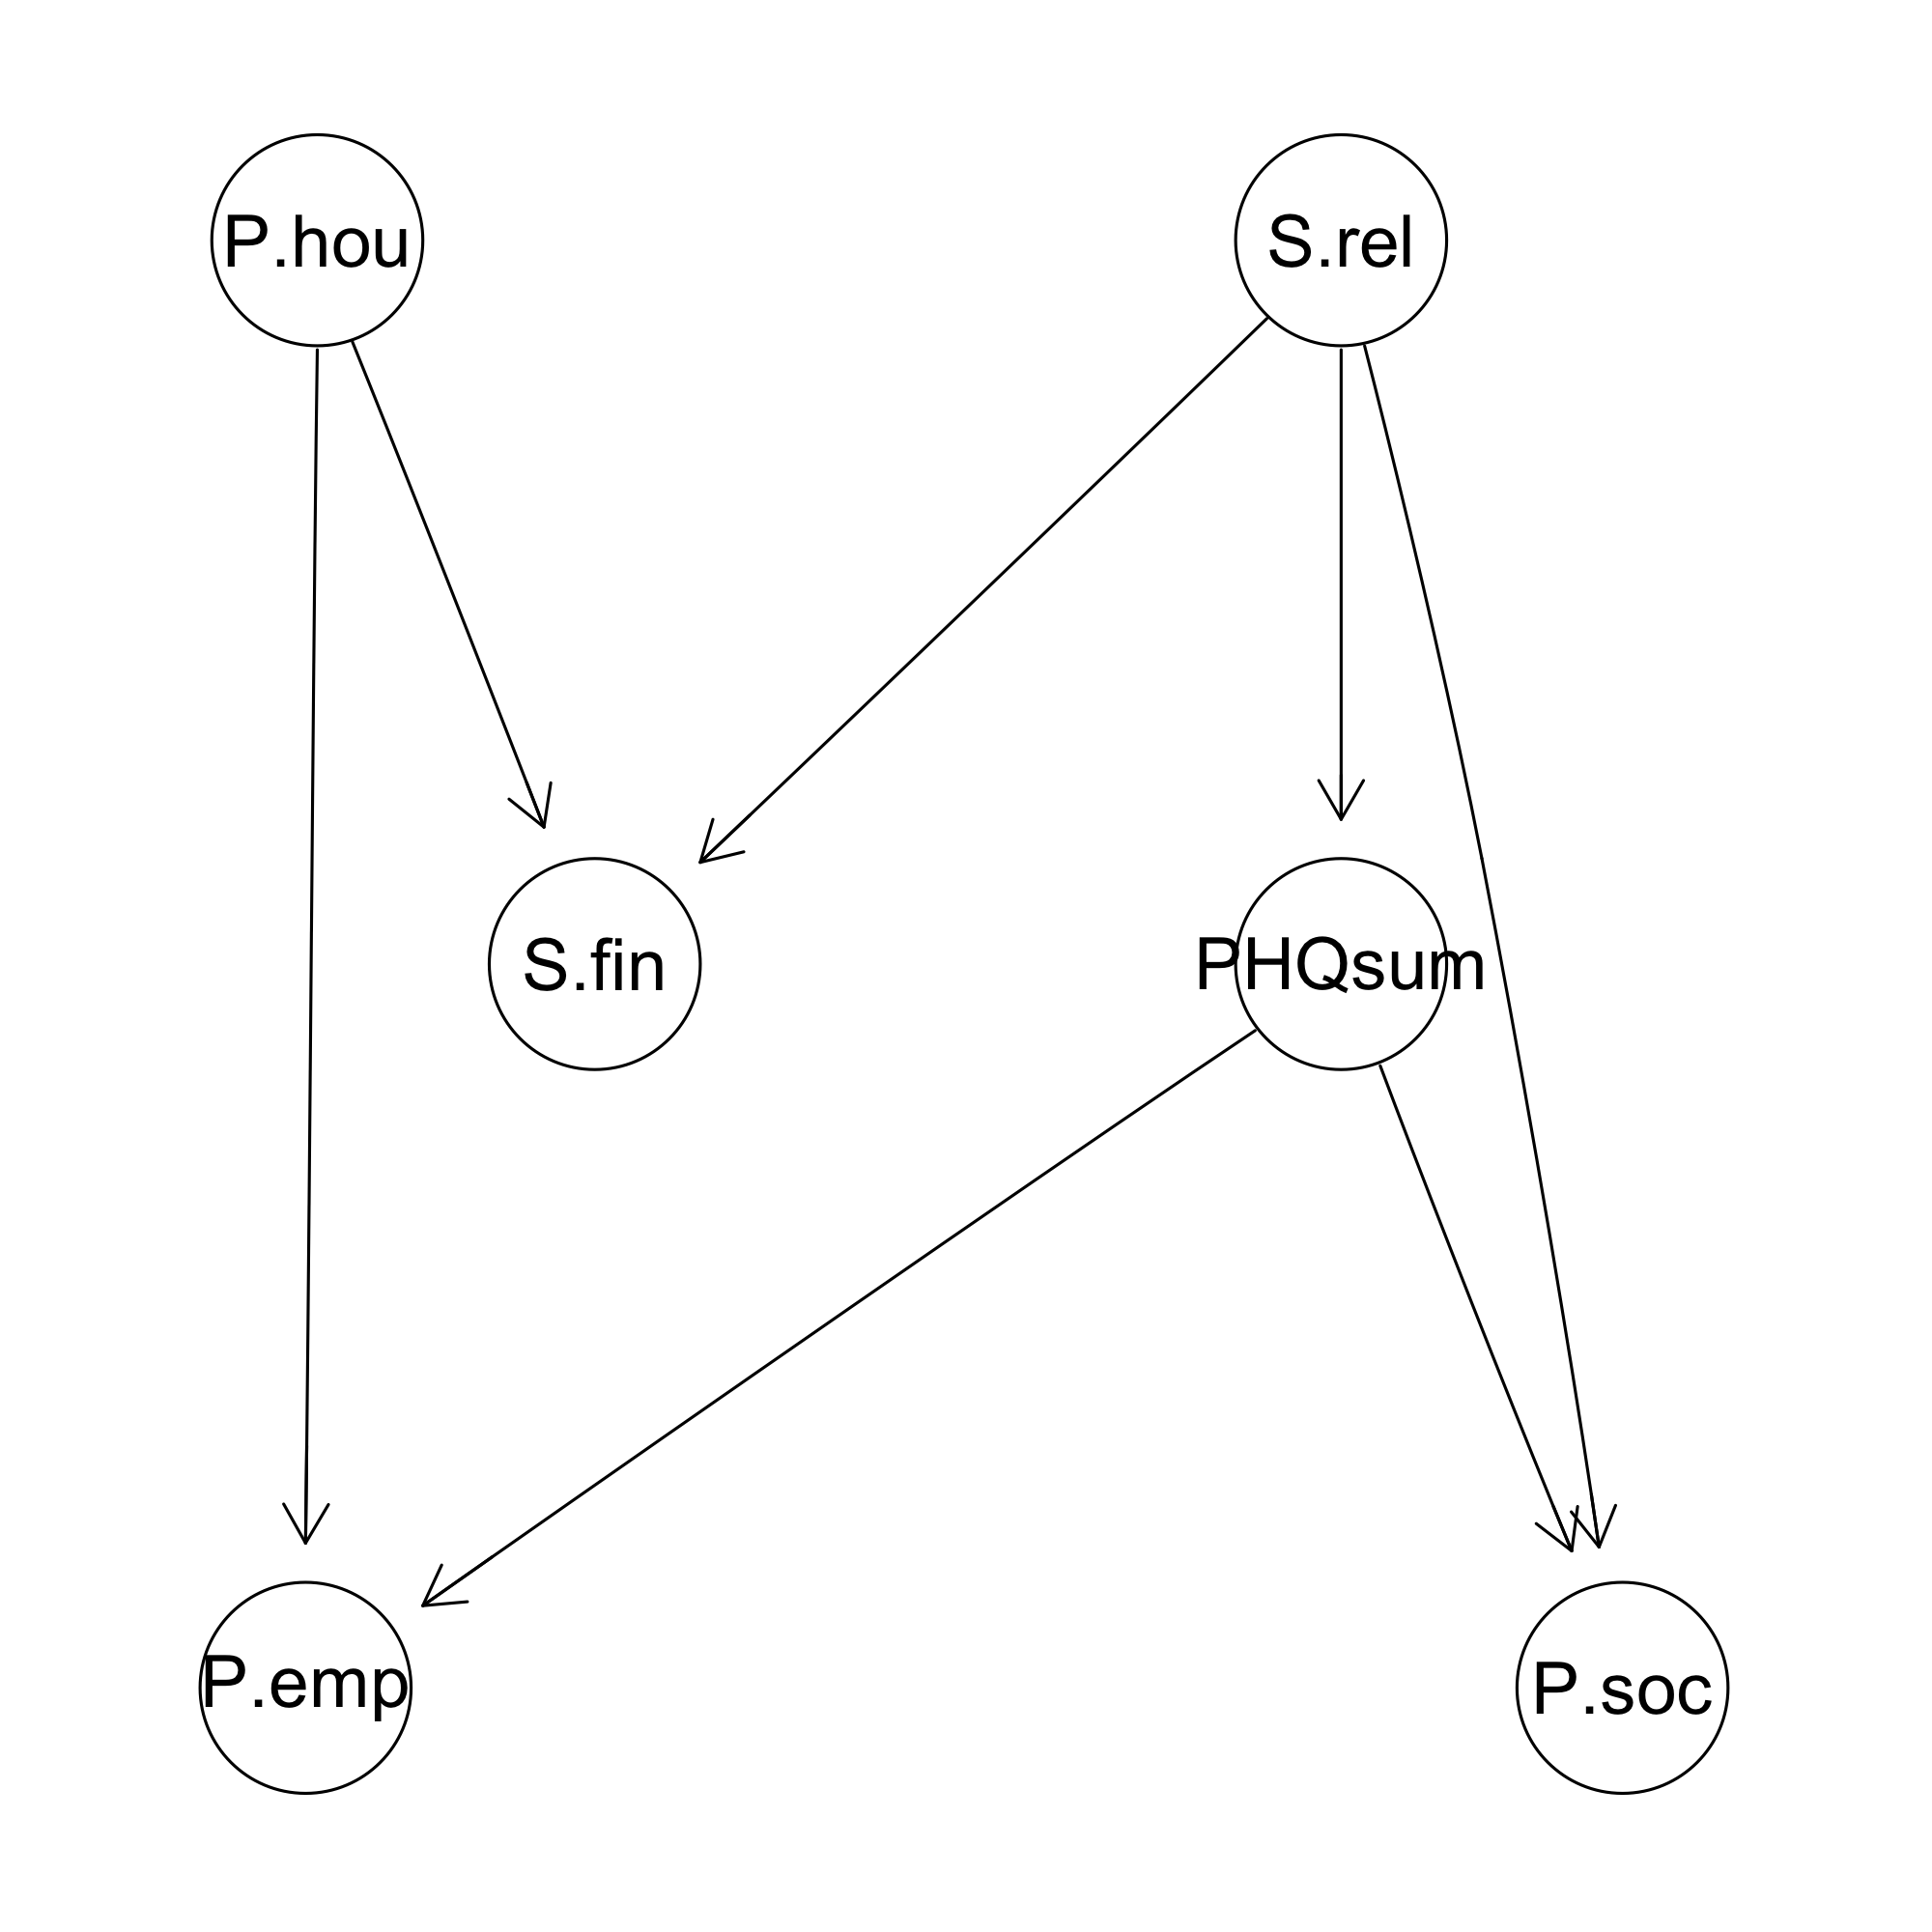
\includegraphics[width=1\textwidth,height=\textheight]{img/sum_PC_RCoTonly.png}

}

\subcaption{\label{fig-pc_sum-2}Using only RCoT}

\end{minipage}%

\caption{\label{fig-pc_sum}Resulting graphs of precarity factors and
depression sum score using PC.}

\end{figure}%

\begin{figure}

\centering{

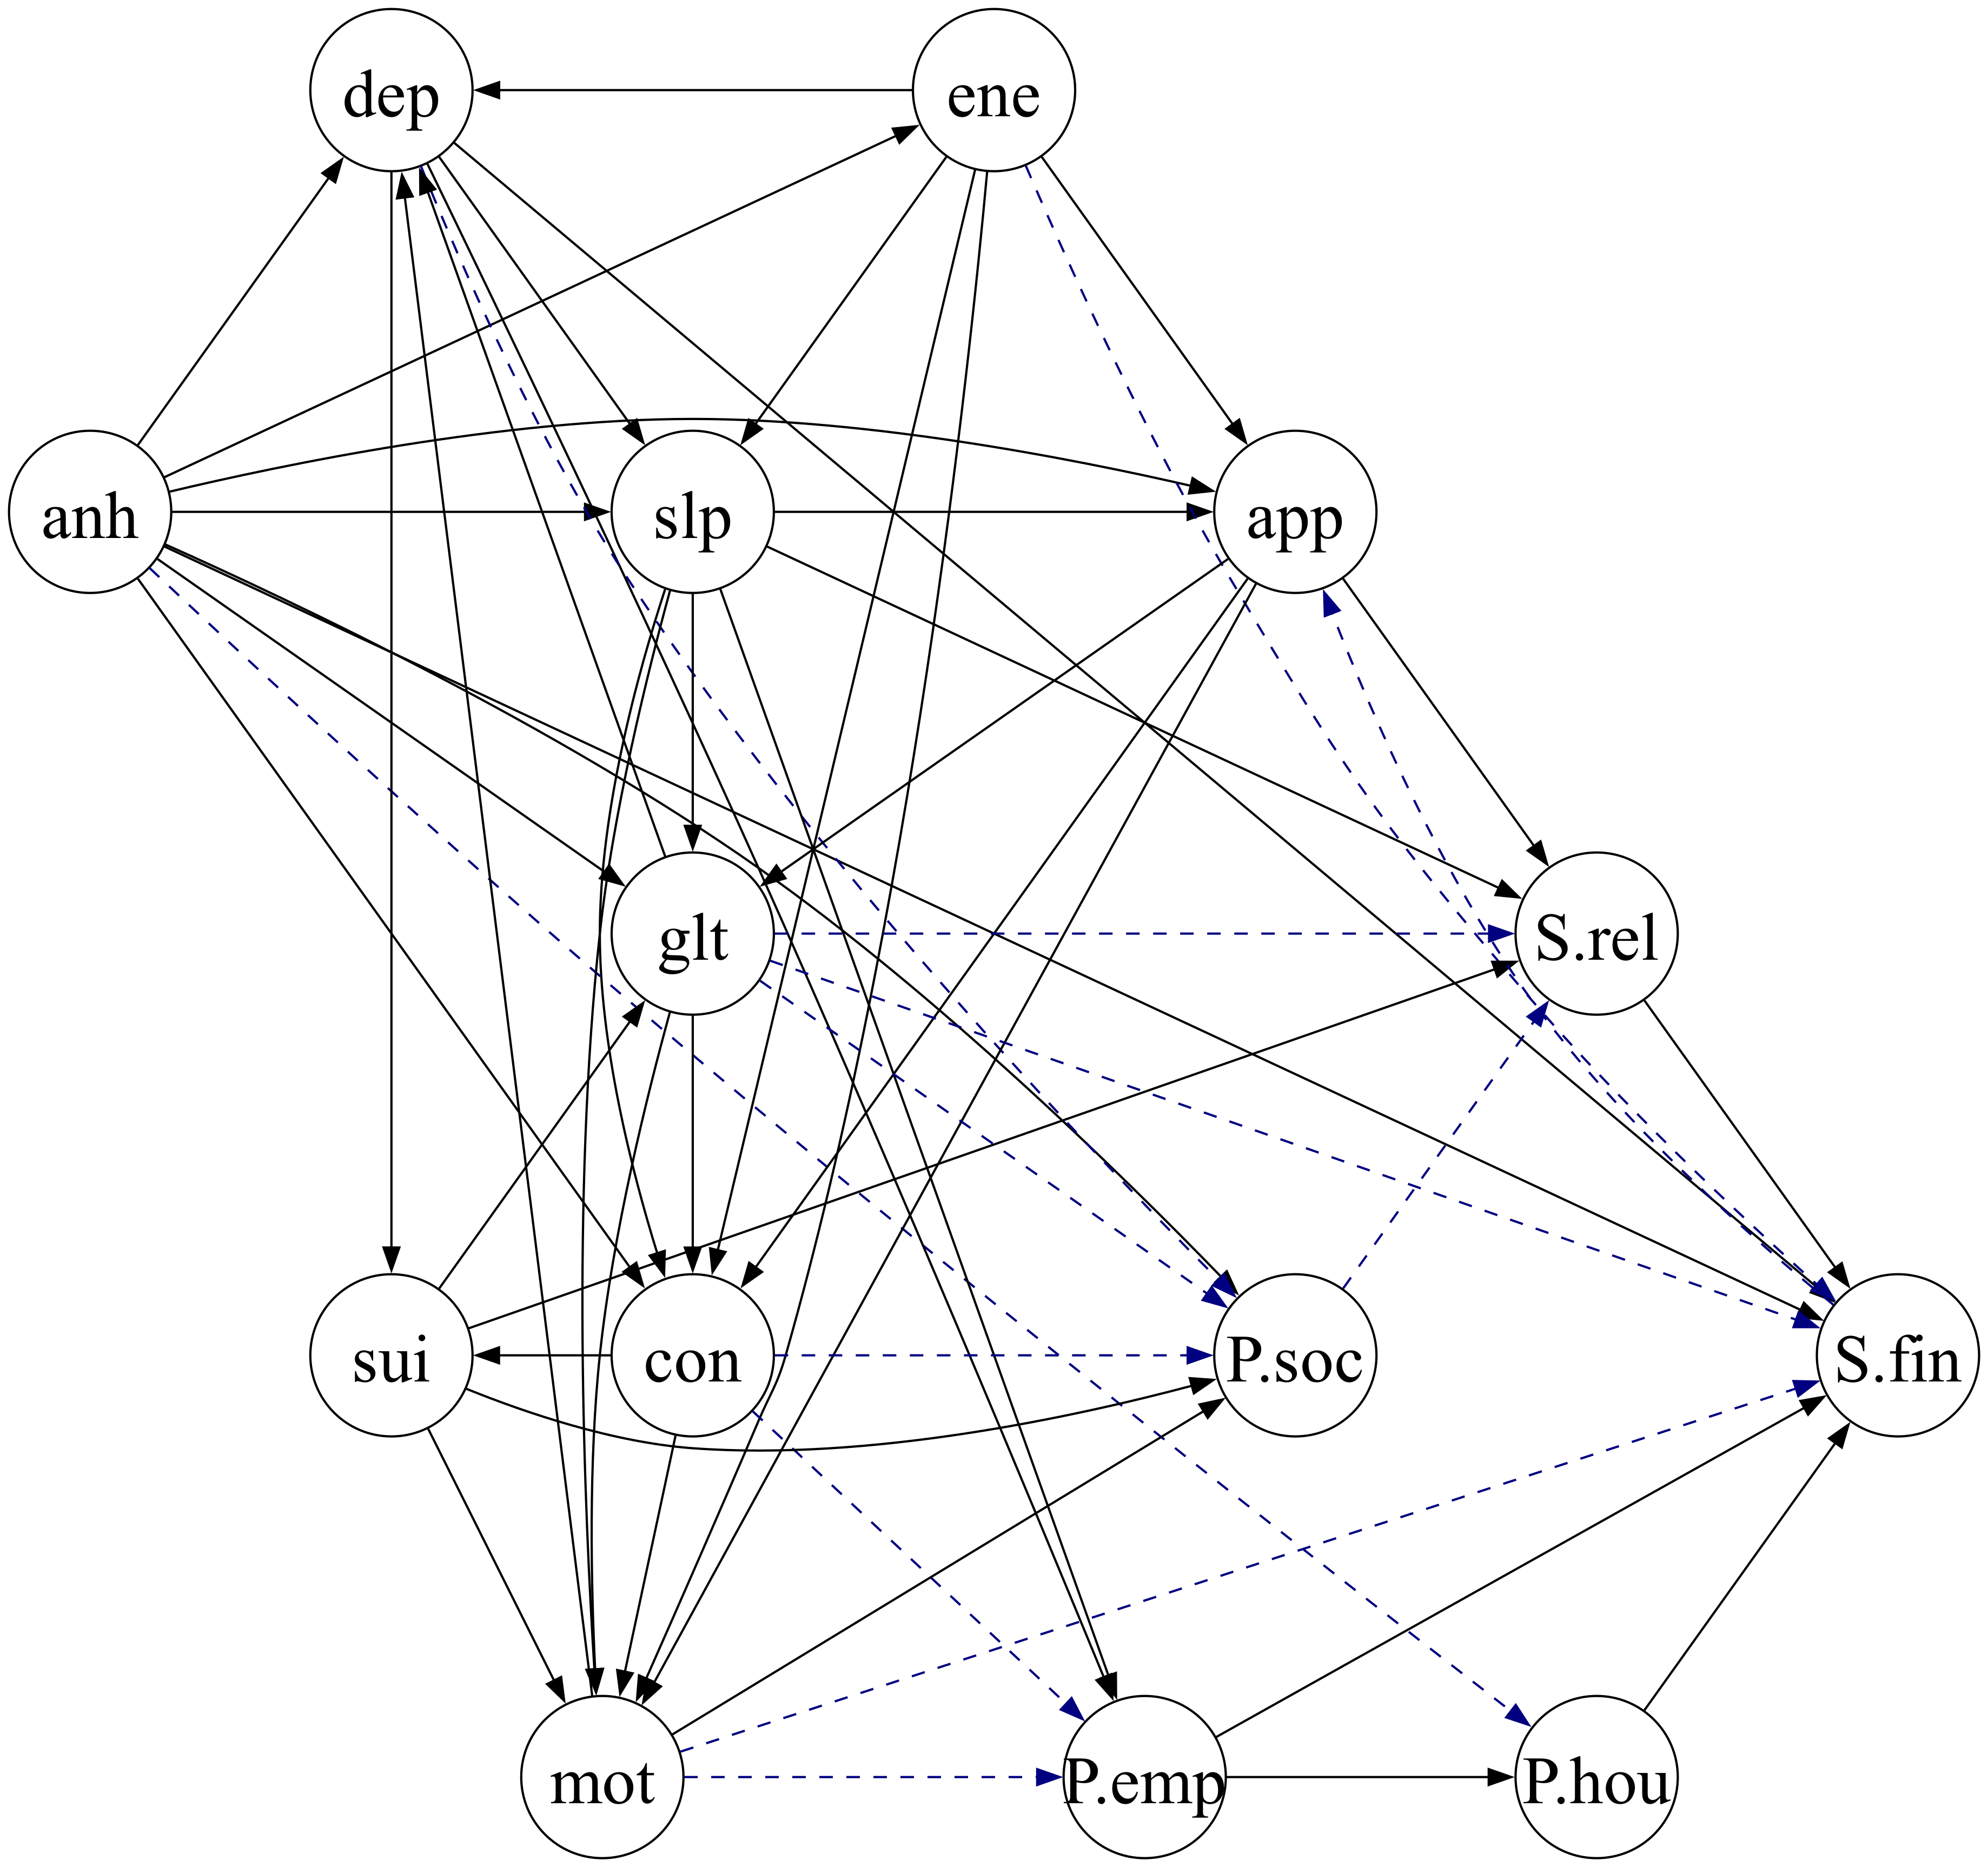
\includegraphics[width=0.6\textwidth,height=\textheight]{img/PC_symptom.png}

}

\caption{\label{fig-pc_sym}Resulting graphs of precarity factors and
individual depression symptoms using PC.}

\end{figure}%

\begin{figure}

\centering{

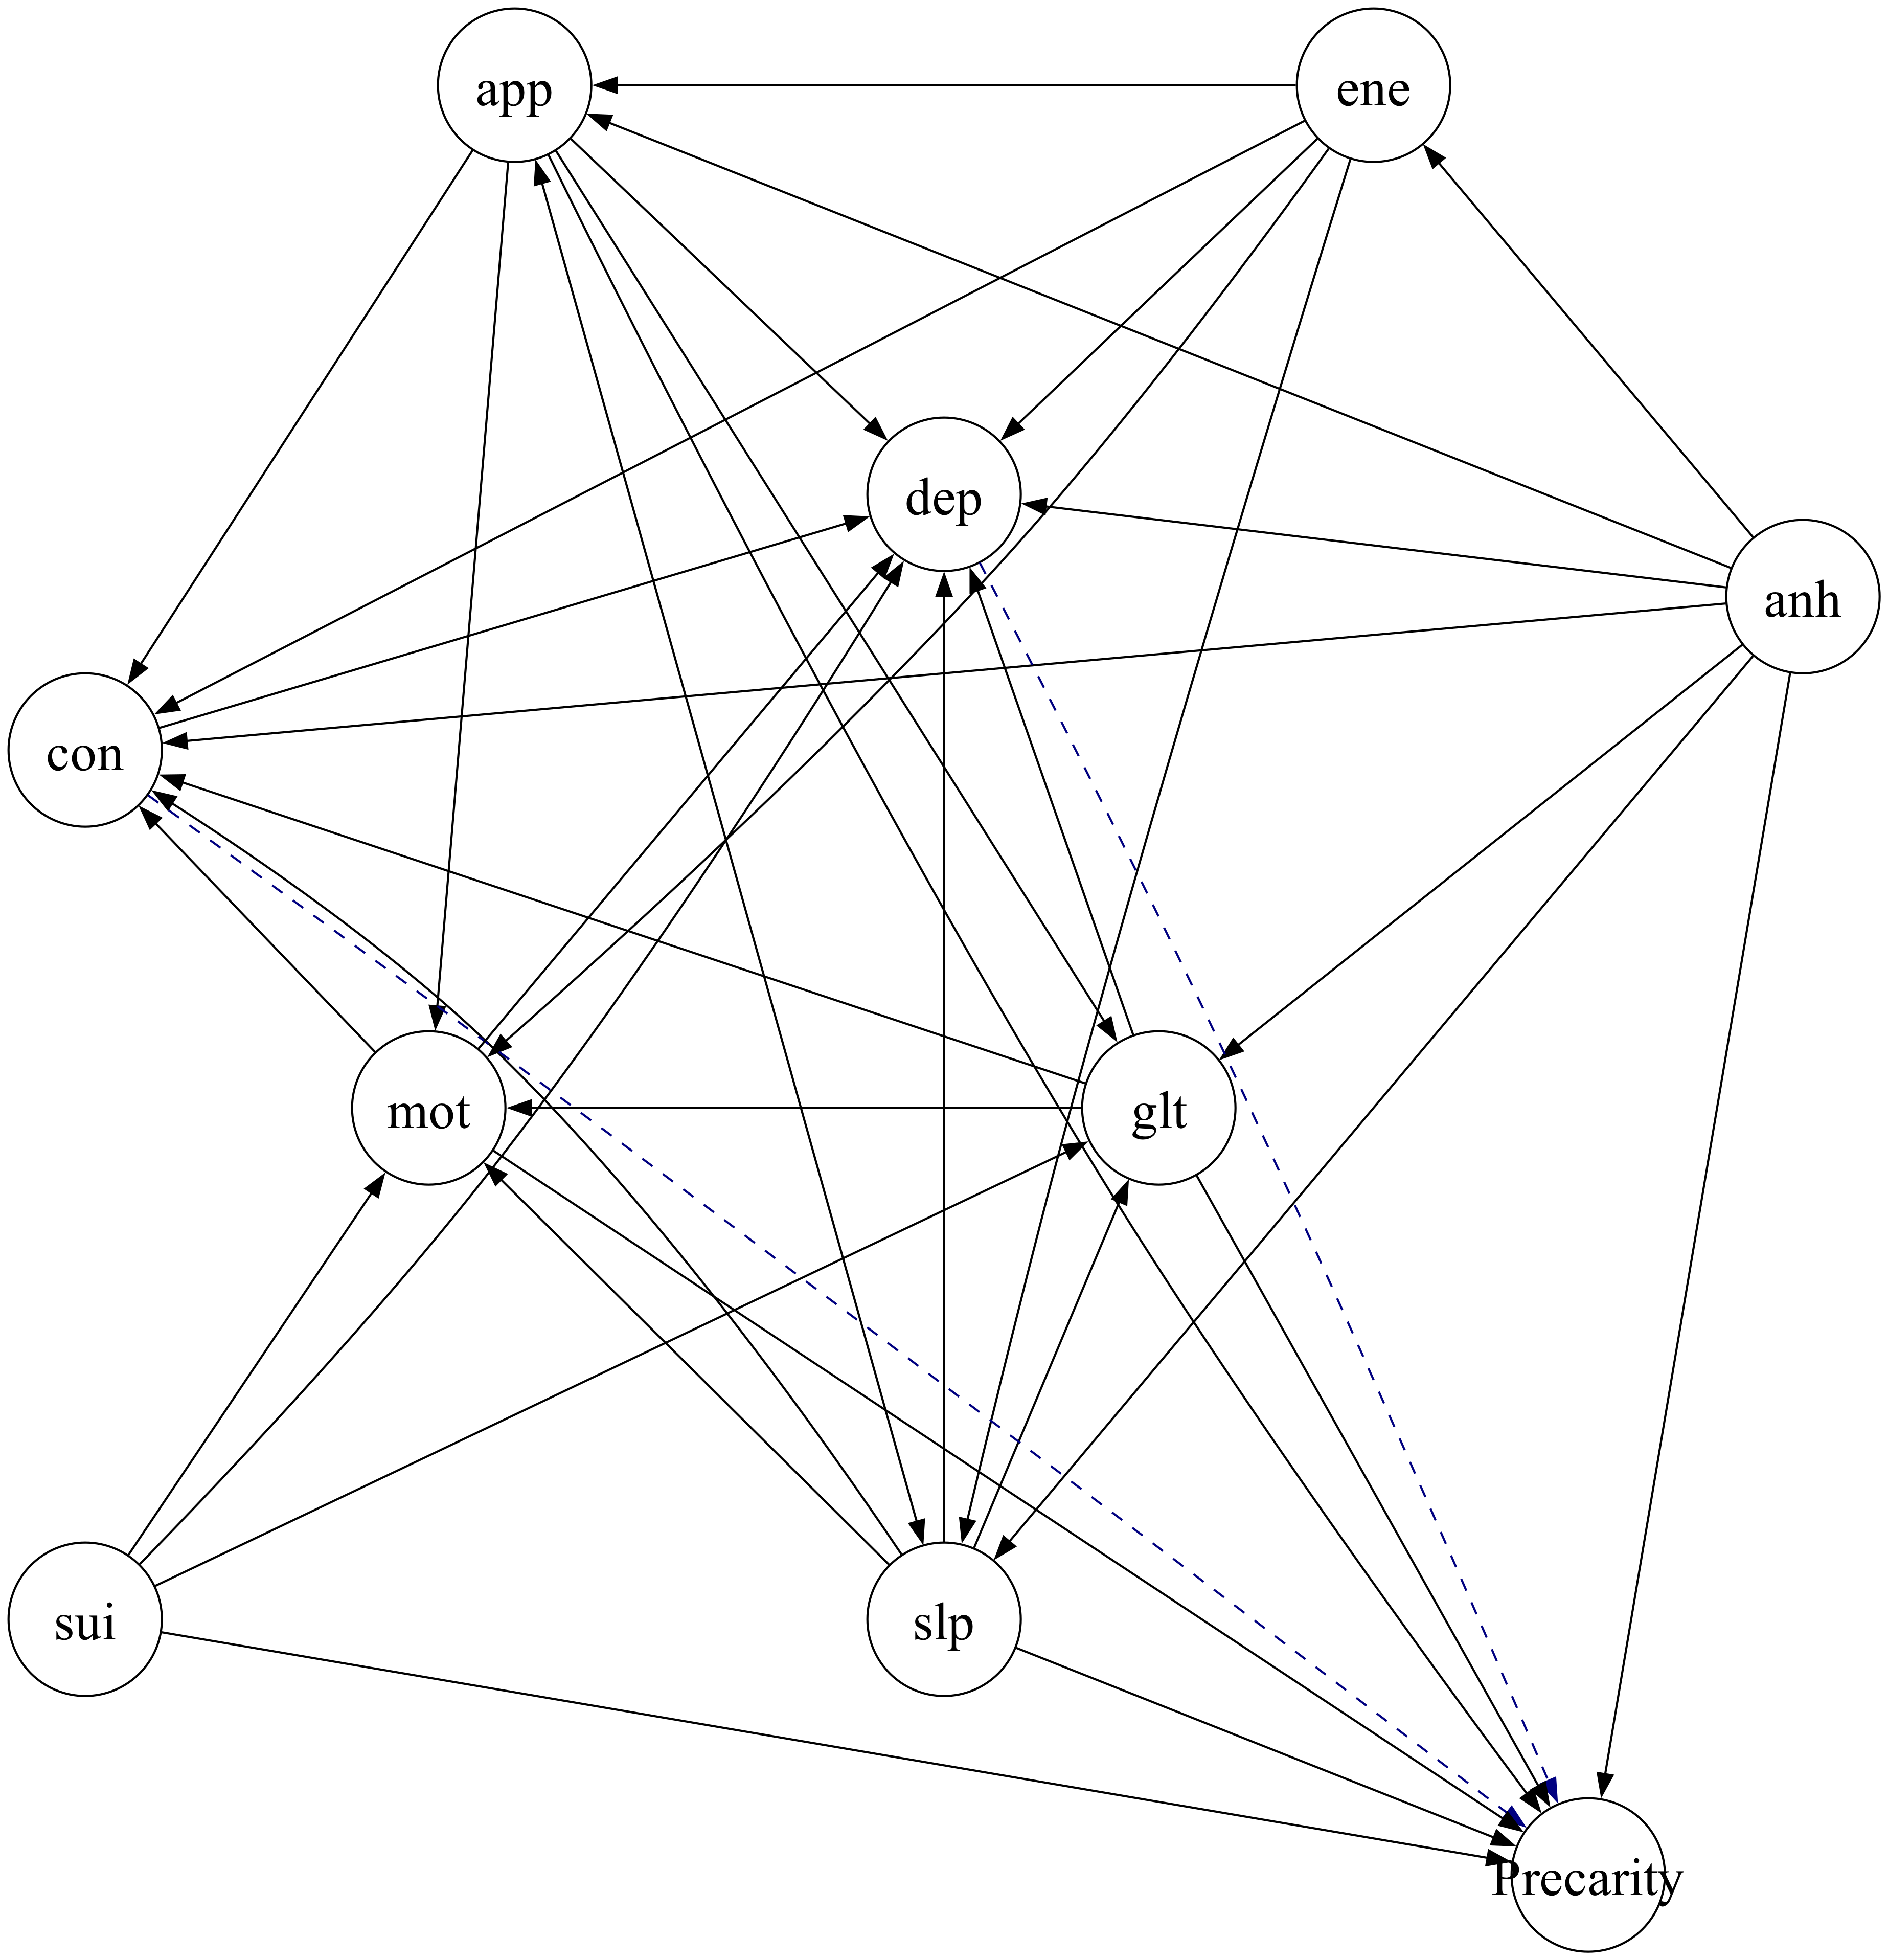
\includegraphics[width=0.6\textwidth,height=\textheight]{img/PC_presum.png}

}

\caption{\label{fig-pc_presum}Resulting graphs of precarity sum score
and individual depression symptoms using PC.}

\end{figure}%

\clearpage

\subsection{Randomized Conditional Independence / Correlation Test (RCIT
\& RCoT)}\label{sec-rcot}

RCIT (Randomized Conditional Independence Test) and RCoT (Randomized
conditional Correlation Test) are advanced methods for scalable
conditional independence (CI) testing, offering computational efficiency
while maintaining the accuracy of kernel-based approaches. These methods
evaluate conditional independence between two variables \(X\) and \(Y\)
given a third variable \(Z\) while addressing computational challenges
inherent in kernel-based CI tests. In this section, we provide a
high-level overview of RCIT and RCoT based on (Strobl et al., 2019).

\subsubsection{Kernel-Based Conditional Independence
Testing}\label{kernel-based-conditional-independence-testing}

Traditional kernel-based CI tests, such as the Kernel Conditional
Independence Test (KCIT), compute dependencies using the Hilbert-Schmidt
Independence Criterion (HSIC) in reproducing kernel Hilbert spaces
(RKHS) (Zhang et al., 2012). KCIT uses the following hypothesis
framework: \[
H_0: X \perp\!\!\!\perp Y \,|\, Z, \quad H_1: X \not\!\perp\!\!\!\perp Y \,|\, Z.
\] The core quantity in KCIT is the partial cross-covariance operator:
\[
\Sigma_{XY \cdot Z} = \Sigma_{XY} - \Sigma_{XZ} \Sigma_{ZZ}^{-1} \Sigma_{ZY},
\] where \(\Sigma_{XY}\) represents the cross-covariance operator
between \(X\) and \(Y\), and
\(\Sigma_{XZ} \Sigma_{ZZ}^{-1} \Sigma_{ZY}\) removes the dependence
mediated by \(Z\).

The squared Hilbert-Schmidt (HS) norm of \(\Sigma_{XY \cdot Z}\) serves
as the test statistic: \[
\|\Sigma_{XY \cdot Z}\|^2_{HS} = 0 \quad \text{if and only if} \quad X \perp\!\!\!\perp Y \,|\, Z.
\]

KCIT estimates residual dependencies using kernel ridge regression: \[
f^*(z) = K_Z (K_Z + \lambda I)^{-1} f(x),
\] where \(K_Z\) is the kernel matrix for \(Z\), \(f(x)\) is the kernel
feature map for \(X\), and \(\lambda\) is the ridge regularization
parameter. The residual function for \(X\) is: \[
f_\text{res}(x) = f(x) - f^*(z) = R_Z f(x),
\] with: \[
R_Z = I - K_Z (K_Z + \lambda I)^{-1}.
\] The kernel matrix for residualized \(X\) is: \[
K_{X \cdot Z} = R_Z K_X R_Z,
\] and similarly for \(Y\), \(K_{Y \cdot Z} = R_Z K_Y R_Z\).

The test statistic is computed as: \[
T_{XY \cdot Z} = \frac{1}{n^2} \text{tr}(K_{X \cdot Z} K_{Y \cdot Z}),
\] which estimates the Hilbert-Schmidt (HS) norm of the partial
cross-covariance operator. To ensure convergence, KCIT scales the
statistic by \(n\): \[
S_K = n T_{XY \cdot Z}.
\] The null hypothesis \(H_0\) is rejected if \(S_K\) exceeds a
threshold determined by permutation or moment-matching-based null
distribution (Lindsay et al., 2000).

\subsubsection{Random Fourier Features
(RFFs)}\label{random-fourier-features-rffs}

Kernel-based methods like KCIT face scalability issues, as they involve
operations on \(n \times n\) kernel matrices, which scale quadratically
with the sample size \(n\). RCIT and RCoT overcome this bottleneck using
\emph{Random Fourier Features (RFFs)} to approximate kernel operations
efficiently.

\paragraph{Bochner's Theorem}\label{bochners-theorem}

Bochner's theorem provides the foundation for RFFs, stating that any
continuous shift-invariant kernel \(k(x, y)\) can be expressed as: \[
k(x, y) = \int_{\mathbb{R}^p} e^{i \omega^\top (x - y)} \, dP_\omega,
\] where \(P_\omega\) is the spectral distribution of the kernel. For
the widely used RBF kernel: \[
k(x, y) = \exp\left(-\frac{\|x - y\|^2}{2\sigma^2}\right),
\] \(P_\omega\) follows a Gaussian distribution:
\(\omega \sim \mathcal{N}(0, \sigma^2 I)\).

\paragraph{RFF Approximation}\label{rff-approximation}

Using Monte Carlo sampling, the kernel function is approximated as: \[
k(x, y) \approx \phi(x)^\top \phi(y),
\] where \(\phi(x)\) is the random Fourier feature mapping: \[
\phi(x) = \sqrt{\frac{2}{D}} \cos(W^\top x + b),
\] with \(W \sim \mathcal{N}(0, \sigma^2 I)\) and
\(b \sim \text{Uniform}(0, 2\pi)\). Here, \(D\) is the number of Fourier
features, which balances computational efficiency and approximation
accuracy.

\subsubsection{Differences Between RCIT and
RCoT}\label{differences-between-rcit-and-rcot}

RCIT and RCoT differ in their test statistics, computational efficiency,
and practical performance, which makes them suited for different
scenarios in causal discovery. RCIT evaluates the Hilbert-Schmidt norm
of the full partial cross-covariance operator, providing a general test
for conditional independence but at a higher computational cost. RCoT
simplifies the process by using the Frobenius norm of a
finite-dimensional residualized cross-covariance matrix, significantly
reducing complexity and improving scalability.

These distinctions are particularly important for large-scale datasets,
where RCoT's computational efficiency makes it a practical choice for
high-dimensional causal discovery tasks.

\paragraph{RCIT: Randomized Conditional Independence
Test}\label{rcit-randomized-conditional-independence-test}

RCIT tests full conditional independence by examining the squared
Hilbert-Schmidt (HS) norm of the partial cross-covariance operator
\(\Sigma_{XY \cdot Z}\): \[
S_K = n T_{XY \cdot Z} = \frac{1}{n} \text{tr}(K_{X \cdot Z} K_{Y \cdot Z}),
\] where \(T_{XY \cdot Z}\) is an empirical estimate of
\(\|\Sigma_{XY \cdot Z}\|^2_{HS}\). The null and alternative hypotheses
are: \[
H_0: \|\Sigma_{XY \cdot Z}\|^2_{HS} = 0, \quad H_1: \|\Sigma_{XY \cdot Z}\|^2_{HS} > 0.
\]

RCIT is a general test for conditional independence but becomes
computationally demanding as the size of \(Z\) increases, due to the
high-dimensional kernel operations required.

\paragraph{RCoT: Randomized Conditional Correlation
Test}\label{rcot-randomized-conditional-correlation-test}

RCoT simplifies the testing process by using a finite-dimensional
partial cross-covariance matrix, avoiding full HS norm calculations.
Instead, it uses the Frobenius norm of the residualized cross-covariance
matrix: \[
S' = n \|C_{AB \cdot C}\|_F^2,
\] where \(C_{AB \cdot C}\) represents the residualized cross-covariance
matrix. The hypotheses are: \[
H_0: \|C_{AB \cdot C}\|_F^2 = 0, \quad H_1: \|C_{AB \cdot C}\|_F^2 > 0.
\]

RCoT is computationally efficient and well-suited for large conditioning
sets (\(|Z| \geq 4\)). Its simplicity enables robust calibration of the
null distribution and improved scalability for high-dimensional data.




\end{document}
